\documentclass[a4paper,12pt,twoside,openright]{book}

\usepackage[utf8]{inputenc} % Encoding
\usepackage[english]{babel} % Lingua
\usepackage{amsmath} % Roba matematica
\usepackage{appendix} % appendices
\usepackage{amsfonts} % Roba matematica
\usepackage{amssymb} % Roba matematica
\usepackage{graphicx} % Per figure
\usepackage{wrapfig} % Per figure con caption
\usepackage{url} % Include gli url
\usepackage[hidelinks]{hyperref} % Include href e rende cliccabili ref
\usepackage{multirow} % Tabelle non omogenee
\usepackage{tabularx} % Tabelle a dimesione fissa e custom
\usepackage{subcaption} % Più figure ravvicinate
\usepackage{float} % Gestione floats (usare H)
\usepackage{listings} % Listare codice sorgente
\usepackage{verbatim} % Commenti multilinea
\usepackage{algorithm} % Pseudocode algorithm display
\usepackage{algpseudocode} % Cool pseudocode algorithm display
\usepackage{fancybox} % Fancy boxes
\usepackage{color} %colori
\usepackage[color=yellow]{todonotes} %todo notes
\usepackage{mathtools} % for prescript
\usepackage{textcomp} %for tilde
\usepackage{hyperref}
\usepackage{fancyhdr}
\usepackage[font=footnotesize,labelfont=bf]{caption}
\usepackage[hmarginratio=2:3,margin=1in]{geometry}
\usepackage[printonlyused, withpage]{acronym} 
\usepackage{booktabs}
\usepackage{array}
\newcolumntype{L}[1]{>{\raggedright\arraybackslash}p{#1}}

\lstset{
	breaklines=true,
	basicstyle=\ttfamily}
\usepackage{setspace}
\definecolor{Code}{rgb}{0,0,0}
\definecolor{Decorators}{rgb}{0.5,0.5,0.5}
\definecolor{Numbers}{rgb}{0.5,0,0}
\definecolor{MatchingBrackets}{rgb}{0.25,0.5,0.5}
\definecolor{Keywords}{rgb}{0,0,1}
\definecolor{self}{rgb}{0,0,0}
\definecolor{Strings}{rgb}{0,0.63,0}
\definecolor{Comments}{rgb}{0,0.63,1}
\definecolor{Backquotes}{rgb}{0,0,0}
\definecolor{Classname}{rgb}{0,0,0}
\definecolor{FunctionName}{rgb}{0,0,0}
\definecolor{Operators}{rgb}{0,0,0}
\definecolor{Background}{rgb}{0.98,0.98,0.98}
\lstdefinelanguage{Python}{
	numbers=left,
	numberstyle=\footnotesize,
	numbersep=1em,
	xleftmargin=1em,
	framextopmargin=2em,
	framexbottommargin=2em,
	showspaces=false,
	showtabs=false,
	showstringspaces=false,
	frame=l,
	tabsize=4,
	% Basic
	basicstyle=\ttfamily\small\setstretch{1},
	backgroundcolor=\color{Background},
	% Comments
	commentstyle=\color{Comments}\slshape,
	% Strings
	stringstyle=\color{Strings},
	morecomment=[s][\color{Strings}]{"""}{"""},
	morecomment=[s][\color{Strings}]{'''}{'''},
	% keywords
	morekeywords={import,from,class,def,for,while,if,is,in,elif,else,not,and,or,print,break,continue,return,True,False,None,access,as,,del,except,exec,finally,global,import,lambda,pass,print,raise,try,assert},
	keywordstyle={\color{Keywords}\bfseries},
	% additional keywords
	morekeywords={[2]@invariant,pylab,numpy,np,scipy},
	keywordstyle={[2]\color{Decorators}\slshape},
	emph={self},
	emphstyle={\color{self}\slshape},
	%
}
\newcommand{\virgolette}[1]{``#1''}
\newcommand{\OT}{OptiTrack}
\newcommand{\PB}{Parrot Bebop 2}
\newcommand{\ML}{Machine Learning}
\newcommand{\R}{\mathbb{R}}
\DeclareMathOperator*{\argmin}{arg\,min}
\setlength\parindent{0pt} % No Indentation
\DeclareMathOperator*{\argmax}{argmax} % argmax
\setlength{\extrarowheight}{0.5mm}
\definecolor{lightgold}{HTML}{FFF4B8} % colore usato per le todonotes 

\newcommand{\titolo}{Implementation of a Laser Turret with 2 Degrees of Freedom, and Applications for Human-Robot Interaction}
\newcommand{\autore}{Gabriele Abbate}
\newcommand{\matricola}{761890}
\newcommand{\relatore}{Prof. Dr. Luca Maria Gambardella}
\newcommand{\correlatoreA}{Dr. Alessandro Giusti}
\newcommand{\correlatoreB}{Dr. Boris Gromov}
\newcommand{\annoaccademico}{2017-18}
\newcommand{\tipolaurea}{Laurea Magistrale in Informatica - Master in Informatics}



\begin{document}
\pagenumbering{Roman}
%\listoftodos

% ============================
%           TITLE
% ============================

\newgeometry{margin=1.5cm}

\begin{titlepage}
	% minipage del logo
	\begin{minipage}{0.30\linewidth}
		
\includegraphics[width=0.7\textwidth]{./img/logo-bicocca-bw.png}\\%%%%%%%%%%%
		
\includegraphics[width=0.7\textwidth]{./img/press-usi-immagini-logo-square.png}%%%%%%%%%%%
	\end{minipage}	
	% minipage header testo
	\begin{minipage}{0.67\linewidth}
		\begin{flushleft}
			{\large Università degli Studi di Milano-Bicocca} \\[0.4cm]
			{\large \bfseries Dipartimento di Informatica, Sistemistica e Comunicazione} \\[0.4cm]
			{\large  \bfseries Corso di laurea Magistrale in Informatica}\\
			\vspace*{1.5cm}
			{\large USI Università della Svizzera Italiana} \\[0.4cm]
			{\large \bfseries Faculty of Informatics} \\[0.4cm]
			{\large  \bfseries Master in Informatics}
		\end{flushleft}
	\end{minipage}
	% titolo
	\begin{center}
		\vspace*{4cm}
		{ \huge \bfseries \titolo} \\[0.1cm]
	\end{center}
	% relatore e corelatore
	\vspace*{2cm}
	\begin{flushleft}
		{\Large \textbf{Supervisor}: \relatore} \\[0.4cm]
		{\Large \textbf{Co-Supervisor}: \correlatoreA} \\[0.4cm]
		{\Large \textbf{Co-Supervisor}: \correlatoreB} \\[0.4cm]
	\end{flushleft}
	% nome
	\vspace*{2cm}
	\begin{flushright}
		{\Large \textbf{Master Thesis of:}} \\[0.4cm]
		{\Large \autore} \\[0.2cm]
		{\Large Student Number \matricola} \\
	\end{flushright}
	% anno accademico
	\vfill
	\begin{center}
		{\Large \textbf{Academic Year 2017-2018}}
		\vspace*{1cm}
	\end{center}
	
\end{titlepage}

\restoregeometry	

% ============================
%       LISTS
% ============================

%Chapter page style redefined
\fancypagestyle{plain}{%
	\fancyhf{} % clear all header and footer fields
	\fancyfoot[C]{\bfseries \thepage} % except the center
	\renewcommand{\headrulewidth}{0pt}
	\renewcommand{\footrulewidth}{0pt}}

\tableofcontents

\clearpage

\begingroup

\let\clearpage\relax
\let\cleardoublepage\relax
\clearpage
\thispagestyle{plain}
\addcontentsline{toc}{chapter}{List of Figures}
\listoffigures


\clearpage
\let\clearpage\relax
\let\cleardoublepage\relax
\thispagestyle{plain}
\addcontentsline{toc}{chapter}{List of Tables}
\listoftables

\clearpage
\let\clearpage\relax
\let\cleardoublepage\relax
\thispagestyle{plain}
\addcontentsline{toc}{chapter}{Listings}
\lstlistoflistings

\clearpage
\endgroup

%% ============================
%         INTRODUCTION
% ============================

\pagestyle{fancy}
\fancyhead{}
\fancyhead[RO, LE]{\slshape Introduction}
\fancyfoot[LO, RE]{\slshape \tipolaurea}
\fancyfoot{}
\fancyfoot[RO, LE]{\thepage}


\pagestyle{fancy}
\fancyhead{}
\fancyfoot{}
\fancyhead[L]{\slshape \leftmark}
\fancyhead[L]{}
\fancyhead[LO, LE]{Chapter \slshape \leftmark}
\fancyhead[RO, RE]{\slshape \rightmark}
\fancyfoot[LO, RE]{\slshape \tipolaurea}
\fancyfoot[C]{}
\fancyfoot[RO, LE]{\thepage}

%Stile dell'Indice
\fancyhead[RO,LE]{\thepage}
\fancyhead[LO]{Index}
\fancyhead[RE]{Index}
\renewcommand{\footrulewidth}{0pt}


% ============================
%          ABSTRACT/INTRODUCTION
% ============================

\chapter*{Introduction\markboth{Introduction}{}} 
\addcontentsline{toc}{chapter}{Introduction}
This thesis describes the development and applications of a laser turret with pan and tilt control: this device can be used to project a laser dot on a given surface (wall and/or floor) and finely control its position by solving the system’s inverse kinematics.

Once its functionality was validated, we used the turret for an human-robot interaction task.  In particular, we considered an existing system in which an operator interacts with a drone using pointing gestures \cite{gromov2018robot}; the system initially determines the relative localization between the two, then allows the operator to control the drone, which follows the indicated location in real time. The existing approach relied on a fast agile robot, and was unsuitable for implementation on slower or larger ground robots.  In this thesis, we demonstrate how the turret can be used with this goal. Figure \ref{fig:preview} gives an idea.
\begin{figure}
	\centering
	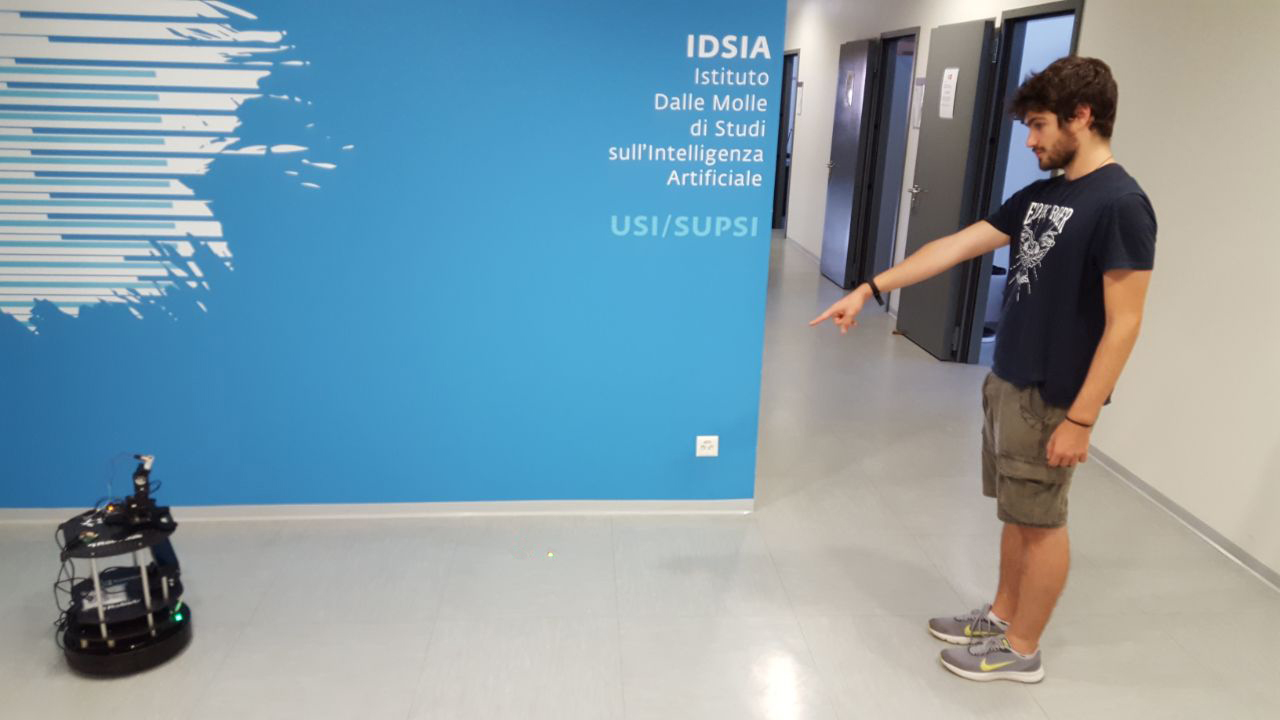
\includegraphics[width=\textwidth]{img/preview.jpg}%
	\caption{System Deployed to Drive a Ground Robot}
	\label{fig:preview}
\end{figure}

Finally, the turret was adopted to efficiently run experiments for fine tuning or validating different components of the system described above, such as the algorithms for relative localization and the algorithms for reconstruction of the pointed direction.  To this end, we ran an experimental campaign involving ten users.

\section*{Motivations and Related Works} \label{sec:related}
Many researches in the field of Human-Robot Interaction (HRI) involve the study of interactions between an operator deployed alongside a robot in an environment they share. That means that a direct-line of sight exists between the two. Many interfaces have been proposed, ranging from standard joysticks (e.g. for low-level control of UAVs) to hands-free gesture-based interfaces based on sensorized armbands~\cite{Wolf2013}, bracelets~\cite{Cacace2016,gromov2018video}, smartwatches~\cite{Villani2017} or voice commands~\cite{Gromov2016}.

The work developed in that thesis is collocated in that context, thus, an overview of related works is useful to understand motivations that stand behind that project.

\subsubsection*{Proximity HRI}
Proximity interaction techniques can take advantage of \emph{pointing gestures} to intuitively express locations or objects with minimal cognitive overhead; this modality has been often used in HRI research e.g. for pick-and-place tasks~\cite{Brooks2006,Droeschel2011,Grossmann2014,Cosgun2015}, labeling and/or querying information about objects or locations~\cite{Brooks2006,Pateraki2014,Akkil2016}, selecting a robot within a group~\cite{Nagi2014a,Pourmehr2013}, and providing navigational goals~\cite{VanDenBergh2011,Abidi2013,Wolf2013,Jevtic2015,Gromov2016,Tolgyessy2017,gromov2018video}.

\subsubsection*{Pointing Based HRI Interface}
First, a differentiation can be made on sensing with respect to the type of sensors involved and their locations with respect to the human: it can be either \emph{external} or based on \emph{wearable} devices.
External sensing is usually based on vision systems, like regular RGB cameras \cite{Pateraki2014,Monajjemi2016}, stereo cameras \cite{Nickel2003}, structured light depth cameras \cite{Cosgun2015} and time-of-flight (ToF) cameras \cite{Droeschel2011}. The wearable sensing is typically realized either with inertial \cite{Wolf2013,Sugiyama2013} or magnetic measurements \cite{Bolt1980,Nickel2003}. 

Our work is an example of wearable sensing, as we exploit a wearable inertial measurement unit (IMU) device. We are interested in such type of sensing because, even if vision-based methods are able to capture rich information about the objects, such as velocity, shape, size and color, they are susceptible to poor lighting conditions, low spatial resolution and may demand high computational resources.
Thus, for proximity interaction, wearable sensing is a very interesting possibility.

In particular, the use of pointing gestures constitutes a very practical and profitable solution, being based on mechanics which are natural for humans. This is why pointing gestures solutions are largely deployed to solve HRI problems and significant research efforts have been devoted to this topic.
In fact, using pointing gestures as an input interface dates back to 1980s, when Bolt presented his now famous work ``Put-that-there''~\cite{Bolt1980}.
In the HRI research, pointing gestures are often used for pick-and-place tasks~\cite{Brooks2006,Droeschel2011,Grossmann2014,Cosgun2015}, labeling and/or querying information about objects or locations~\cite{Brooks2006,Pateraki2014,Akkil2016}, selecting a robot within a group~\cite{Nagi2014a,Pourmehr2013}, and providing navigational goals~\cite{VanDenBergh2011,Abidi2013,Wolf2013,Jevtic2015,Gromov2016,Tolgyessy2017}.

Providing navigational goals is exactly the field in which our system finds one of its main applications and this is why we are now going to mention more works related to that task. Fist, however, it is worth to say that one important issue to be solved in natural human-robot interaction that involves pointing is a perception of the user's gestures. This can be a responsibility of a robot, i.e. the recipient of the message, as well as of a group of cooperatively-sensing robots~\cite{Giusti2012,Pourmehr2013}; of the environment~\cite{zivkovic2008toward}; or, as in our case, of a device worn by the user~\cite{Sugiyama2013,Wolf2013,Gromov2016}. The first approach is the most popular in HRI research. However, it presents important challenges to solve the perception problem, and requires the robot to consistently monitor the user. Relying on sensors placed in the environment relaxes the requirements on the robots, but limits the applicability of the system to properly instrumented areas; in both cases, the positions being pointed at need to be inferred by external observation, which is typically performed with cameras or RGB-D sensors.

\subsubsection*{Providing Navigational Goals}
Van Den Bergh et al. \cite{VanDenBergh2011} used pointed directions to help a ground robot to explore its environment. The robot continuously looks for a human in its vicinity and once detected begins the interaction. Using an RGB-D sensor (Microsoft Kinect) the system detects human's hand and wrist. A vector connecting the center of the hand and the wrist is then projected on the ground, giving a principal exploration direction. Finally, the next exploration goal is automatically selected from a set of possible goals with respect to an instantaneous occupancy grid acquired by the robot. 

Similarly to the previous work, Abidi et al. \cite{Abidi2013} use a Kinect sensor to extract pointed directions. Navigation goals are continuously sent to the ground robot, which reactively plans its motion and thus allows the user to correct his input on the fly. The main drawback, however, is that the robot has to ``keep an eye'' on the user in order to reach the final target. To estimate pointed locations authors suggest two approaches: (1)~a vector originating from the elbow and passing the hand/finger, and (2)~a vector originating from the eyes and also passing the hand/finger.

Jevtic at al. \cite{Jevtic2015} experimentally compared several interaction modalities in the user study of 24 participants. A ground robot equipped with a Kinect and other sensors was used. The study compares three interaction modalities: direct physical interaction (DPI), person following, and pointing control in area- and waypoint-guidance tasks. The DPI modality requires the user to push the robot by hands, the torques generated at motors are measured via electrical current and then are fed to a friction-compensation controller that drives the robot in the appropriate direction. The person following modality makes the robot to follow the user at a safe distance, the user can stop the robot at any time by raising her left hand above the left elbow and thus can control the robot's precise location. The pointing modality allows the user to command the robot's position with a pointing gesture, where the target location is calculated from the intersection of the ground plane with a line passing through the right elbow and the right hand of the user.
The authors measured task completion times, accuracy, and workload (with NASA-TLX questionnaire). Reported results show that the DPI modality is systematically better than the other modalities for all the metrics, while the pointing control shows the worst results.

Such a low performance of the pointing interface can be explained by a lack of appropriate feedback and a time-sparse nature of the implemented gesture control: the user issues a single command to drive the robot to a goal and see where the system ``thinks'' he was pointing at only when the robot reaches the target, therefore, the user is unable to efficiently correct the robot's position. This problem is nicely solved by our system, as it provides a real-time feedback to user pointing with a laser pointer, making him able to understand where the system thinks he is pointing and also correct any misalignment. Anyway, an important difference is that we are not driving the robot in real time, but just sending a goal point for it to reach.

Problems reported in the study by Jevtic at al. \cite{Jevtic2015} are further aggravated by an inherently limited precision of a chosen pointing model (elbow-hand). As reported by many other works (see~\cite{Abidi2013,Nickel2007,Droeschel2011}), including those from the psychology research (see~\cite{Taylor1988,Herbort2016}), a more appropriate model would be a line that passes through the head and the fingertip. This is exactly the model we use for that thesis.

\subsubsection*{Wearable Sensors}
An alternative approach to a perception of pointing gestures is wearable sensors, as we mentioned before. 

Sugiyama et al. \cite{Sugiyama2013} developed a wearable visuo-inertial interface for on-site robot teaching that uses a combination of monocular camera and IMU to capture hand gestures in the egocentric view of the user. The camera is also used for a monocular simultaneous localization and mapping (SLAM), which allows to localize the user with respect to a common with the robot coordinate frame.

Wolf et al. \cite{Wolf2013} suggest a gesture-based interface for a robot control, that is based on a device they call BioSleeve, a wearable device placed on the user's forearm and comprised of a set of dry-contact surface electro-myography sensors (EMGs) and an IMU. Optionally, the authors suggest to strap an additional IMU sensor on the upper arm to be able to perform a model-based arm pose reconstruction for pointing gestures. However, no information is given on how a user would localize herself with respect to the robot in order to control its position.

A work by Villan et al. \cite{Villani2017} suggests to use a single smartwatch device to control a drone. The system provides two interfaces: high-level commands and velocity commands.

Cacace et al. \cite{Cacace2016} demonstrate a multi-modal human-robot interface used for interaction in search and rescue missions. The operator is equipped with a Myo armband used for gestures, headset for voice commands, and a tablet with a touch screen.

\section*{Document Structure}
The rest of the document is structured in chapter as follows:
\begin{itemize}
    \item \textbf{Chapter 1 - Models Specification}  All the geometric models and formulas on which the system is based are explained. This includes turret model, human pointing model and relative localization procedure;
    \item \textbf{Chapter 2 - Hardware Implementation}  We introduce all the hardware components involved in the development of the presented system: servo motors and interface board for the turret, arm IMU devices and the ground robot used for demonstrations;
    \item \textbf{Chapter 3 - Software Implementation} We give an overview of the main libraries used and then describe the entire project software implementation;
    \item \textbf{Chapter 4 - Experiments and Applications} We describe the experiments the turret system allowed us to perform and show possible application scenarios developed;
    \item \textbf{Chapter 5 - Conclusion and Future Work} We make a brief recap of the thesis, draw some conclusions and report eventual further improvements or possible works.
\end{itemize}

\fancyhead[RO,LE]{\thepage}
\fancyhead[LO]{Introduction}
\fancyhead[RE]{Introduction}
\renewcommand{\footrulewidth}{0pt}

% ============================
%           CHAPTERS
% ============================

\renewcommand{\chaptermark}[1]{\markboth{\thechapter.\ #1}{}}
\renewcommand{\sectionmark}[1]{\markright{\thesection.\ #1}}

\cleardoublepage
\fancyhead[RO,LE]{\bfseries \thepage}
\fancyhead[LO]{\bfseries \rightmark}
\fancyhead[RE]{\bfseries Chapter \leftmark}
\renewcommand{\footrulewidth}{0pt}

\pagenumbering{arabic}

\chapter{Model Specification}
\label{chap:1} 
In this chapter we describe the abstract models used to shape all the three parts of the system. (FARE QUI UN ELENCO? torretta, puntamento, kobuki)
\section{Turret Model}
Degree of Freedom (DoF) is the number of independent parameters that define the configuration of a mechanical system. In our case, we wanted to build a two DoF Pan \& Tilt turret. That means that our parameters are two angles. In a 3D reference system, \textbf{pan} is the horizontal angle about the upright Z axis, \textbf{tilt} is the vertical angle about the rotated Y axis, as in figure \ref{fig:panTilt}.
Our final goal is to be able to define the direction of a laser ray mounted on top of the turret, so that we can control the position of the projected laser dot on a given surface, by solving the system's inverse kinematics.\\
\begin{figure}
	\centering
	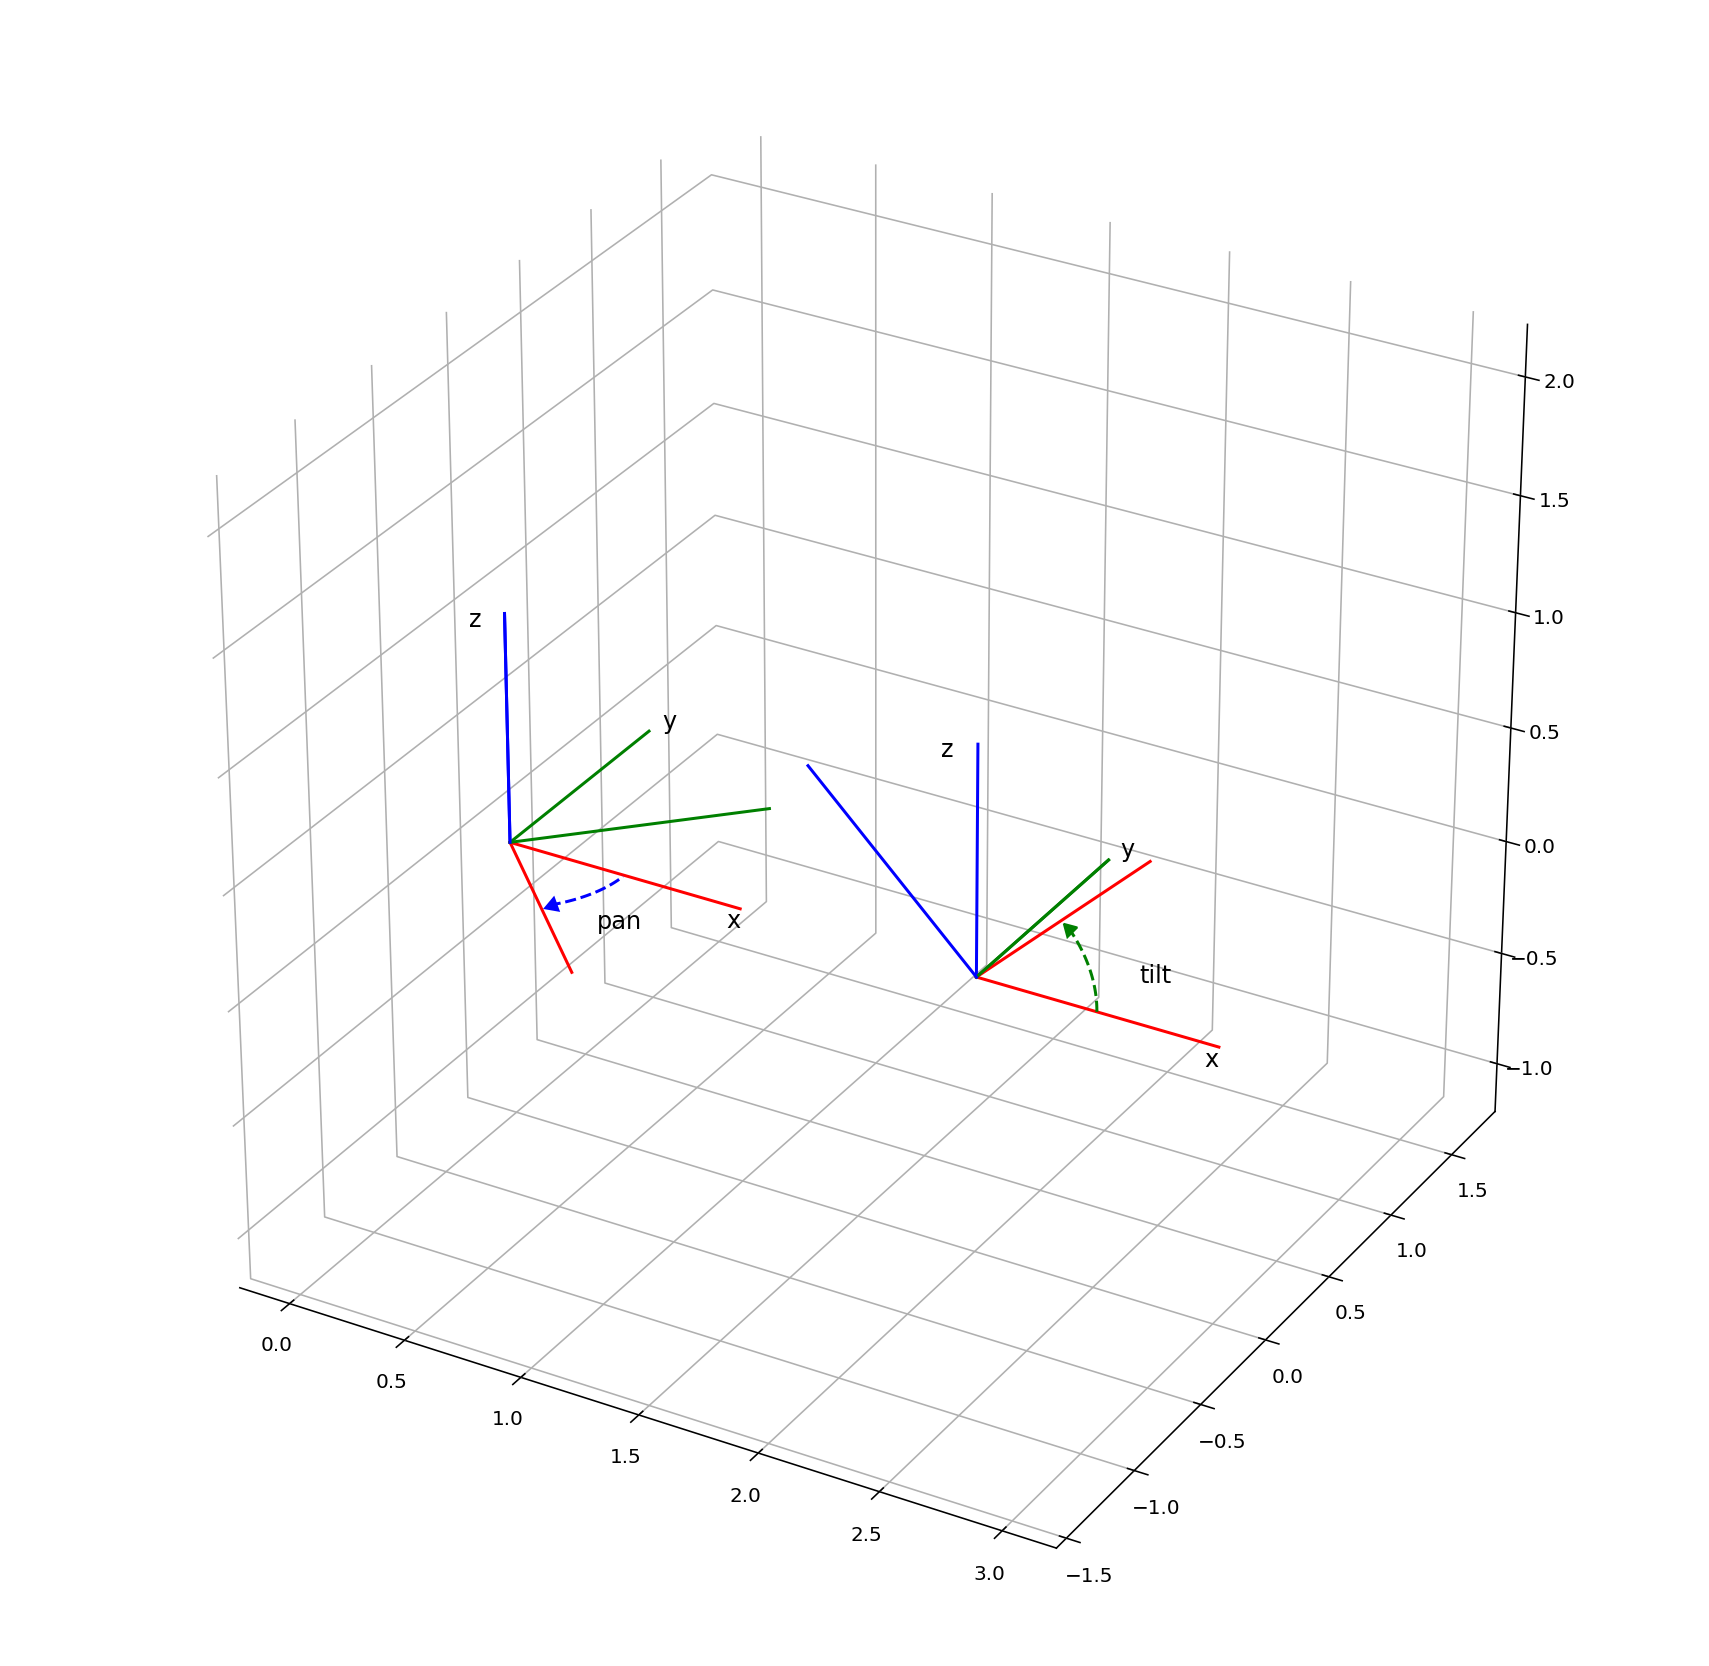
\includegraphics[width=\textwidth]{img/panTilt.png}%
	\caption{Pan and Tilt}
	\label{fig:panTilt}
\end{figure}
For those purposes, we have built two different turrets. Since the model of the first one is slightly simpler than the second, we will start describing the former, which turns out to be helpful to understand the latter. We will focus on the case in which the laser must be projected on the ground.

\subsection{First Model}\label{subs:firstModel}
First, figure \ref{fig:firstModelRefFrame} helps us understand how we have shaped the model to match the physical structure of the turret. We have three reference frames. The \textbf{base\_frame} is fixed and is the one in which we define the coordinates of the projected point. \textbf{pan\_frame} and \textbf{tilt\_frame} are the frames used to represent our revolute joints.
\textbf{H} is the height of the turret, which is known. Note that the convention used for the frame is the following:
\begin{itemize}
    \item red is the x axis;
    \item green is the y axis;
    \item blue is the z axis.
\end{itemize}
Thus, we consider the laser ray to be a prolongation of the x axis of the \textbf{tilt\_frame}. \\
Figure \ref{fig:firstModelPanTilt} shows what we want to be able to do: given the \textit{x}, \textit{y} and \textit{z} of the laser point we want to set \textbf{pan} and \textbf{tilt} angles accordingly. In order to do so, firstly we will solve the forward kinematic, then the inverse will be easily derived.
\subsubsection{Forward Kinematic}
The forward kinematic should take as input our parameters (i.e. \textbf{pan} and \textbf{tilt}) and then return the coordinates of the laser projected point into \textbf{base\_frame} reference. 
Note that, since we are controlling the direction of an infinite ray, in order to obtain a unique (\textit{x, y, z}) triple, we must intersect such ray with a plane defined by the triple (\textit{0, 0, z}). In the forward kinematic equations this can be obtained by assuming that we know the \textit{z} of the point we want. Another option could be to assume that \textit{z} is zero, since we are considering the laser projection on the floor (i.e. on the \textbf{base\_frame}). \\
As well as what is already defined in figure \ref{fig:firstModelPanTilt}, we must add:
\begin{itemize}
    \item \textbf{L} as the distance from the \textbf{pan\_frame} origin to the projection of the laser point on the \textbf{base\_frame};
    \item \textbf{D} as the distance from the \textbf{tilt\_frame} origin to the laser point.
\end{itemize}
First, note that the \textbf{pan} angle does not depends on the \textit{z} coordinate, so, starting from:
\begin{align}
	D=& \frac{H-z}{\cos{(tilt)}} \label{eq:d}\\
	L=& \sqrt{(H-z)^2 + D^2}
\end{align}
We can easily obtain laser point coordinates:
\begin{align}
	x=& L\cos{(pan)}\label{eq:x}\\
	y=& L\sin{(pan)} \label{eq:y}
\end{align}

\begin{figure}
	\centering
	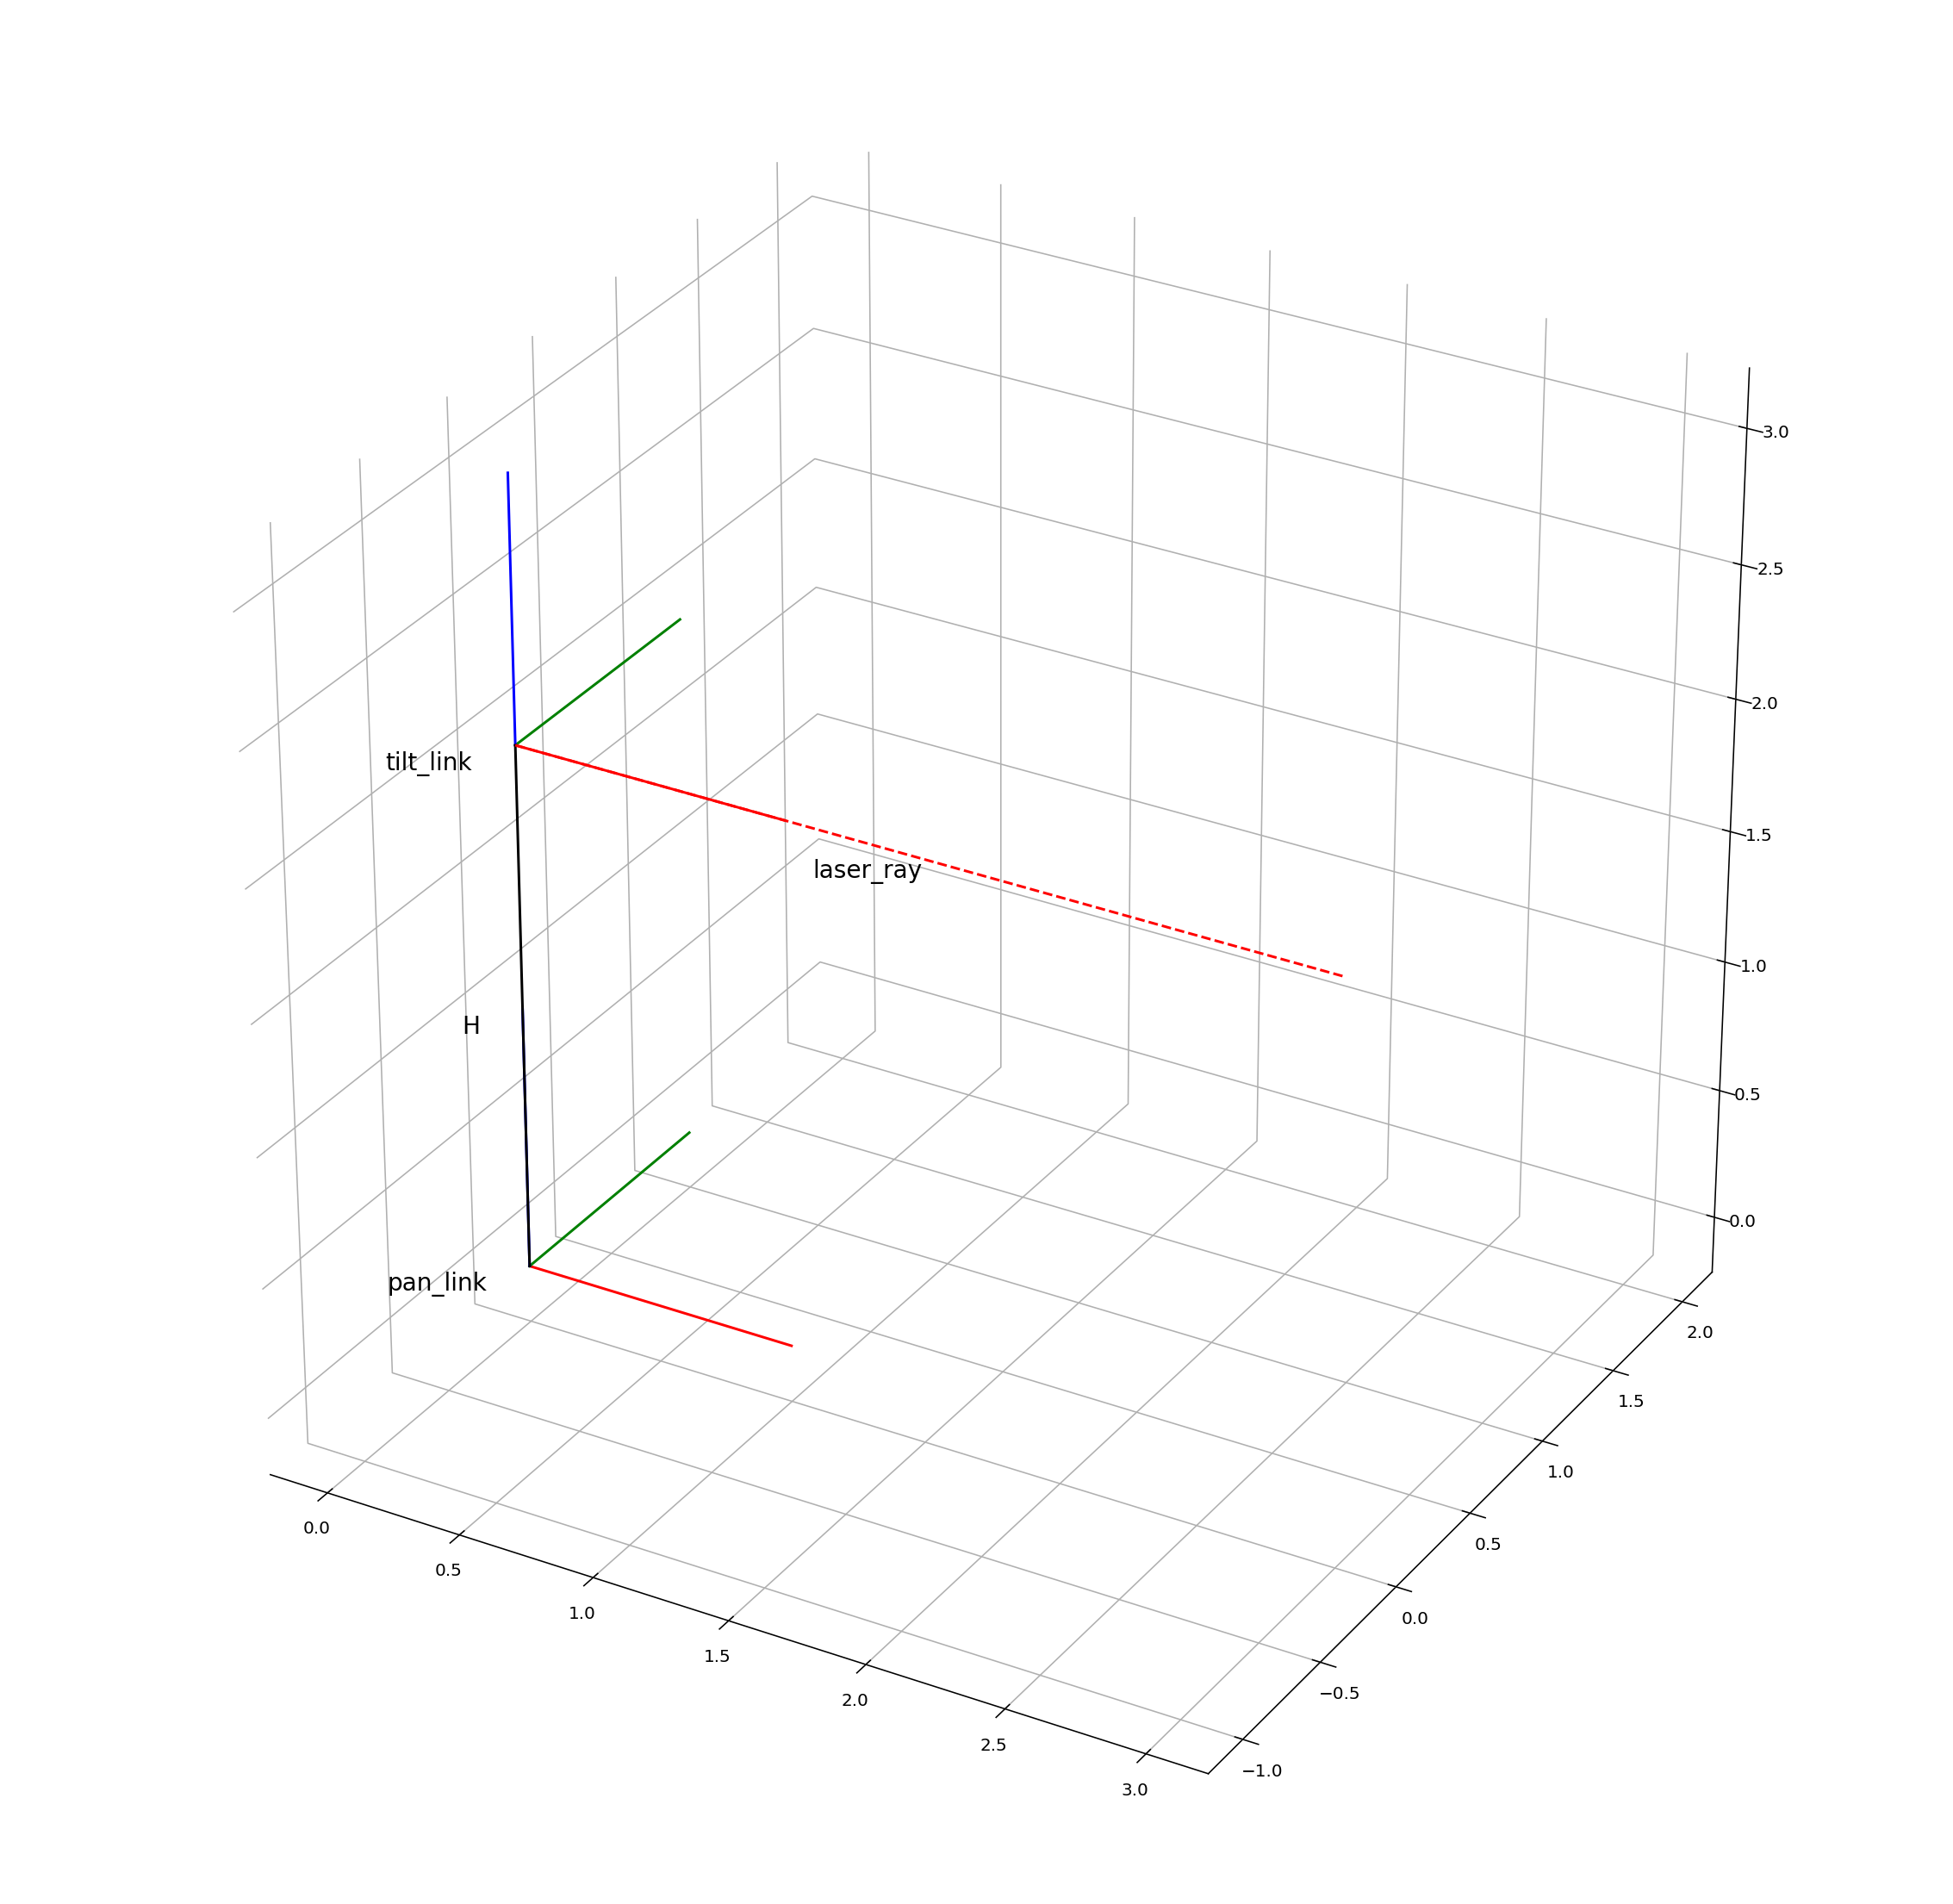
\includegraphics[width=\textwidth]{img/firstModel.png}%
	\caption{First Model, Reference Frames}
	\label{fig:firstModelRefFrame}
\end{figure}
\begin{figure}
	\centering
	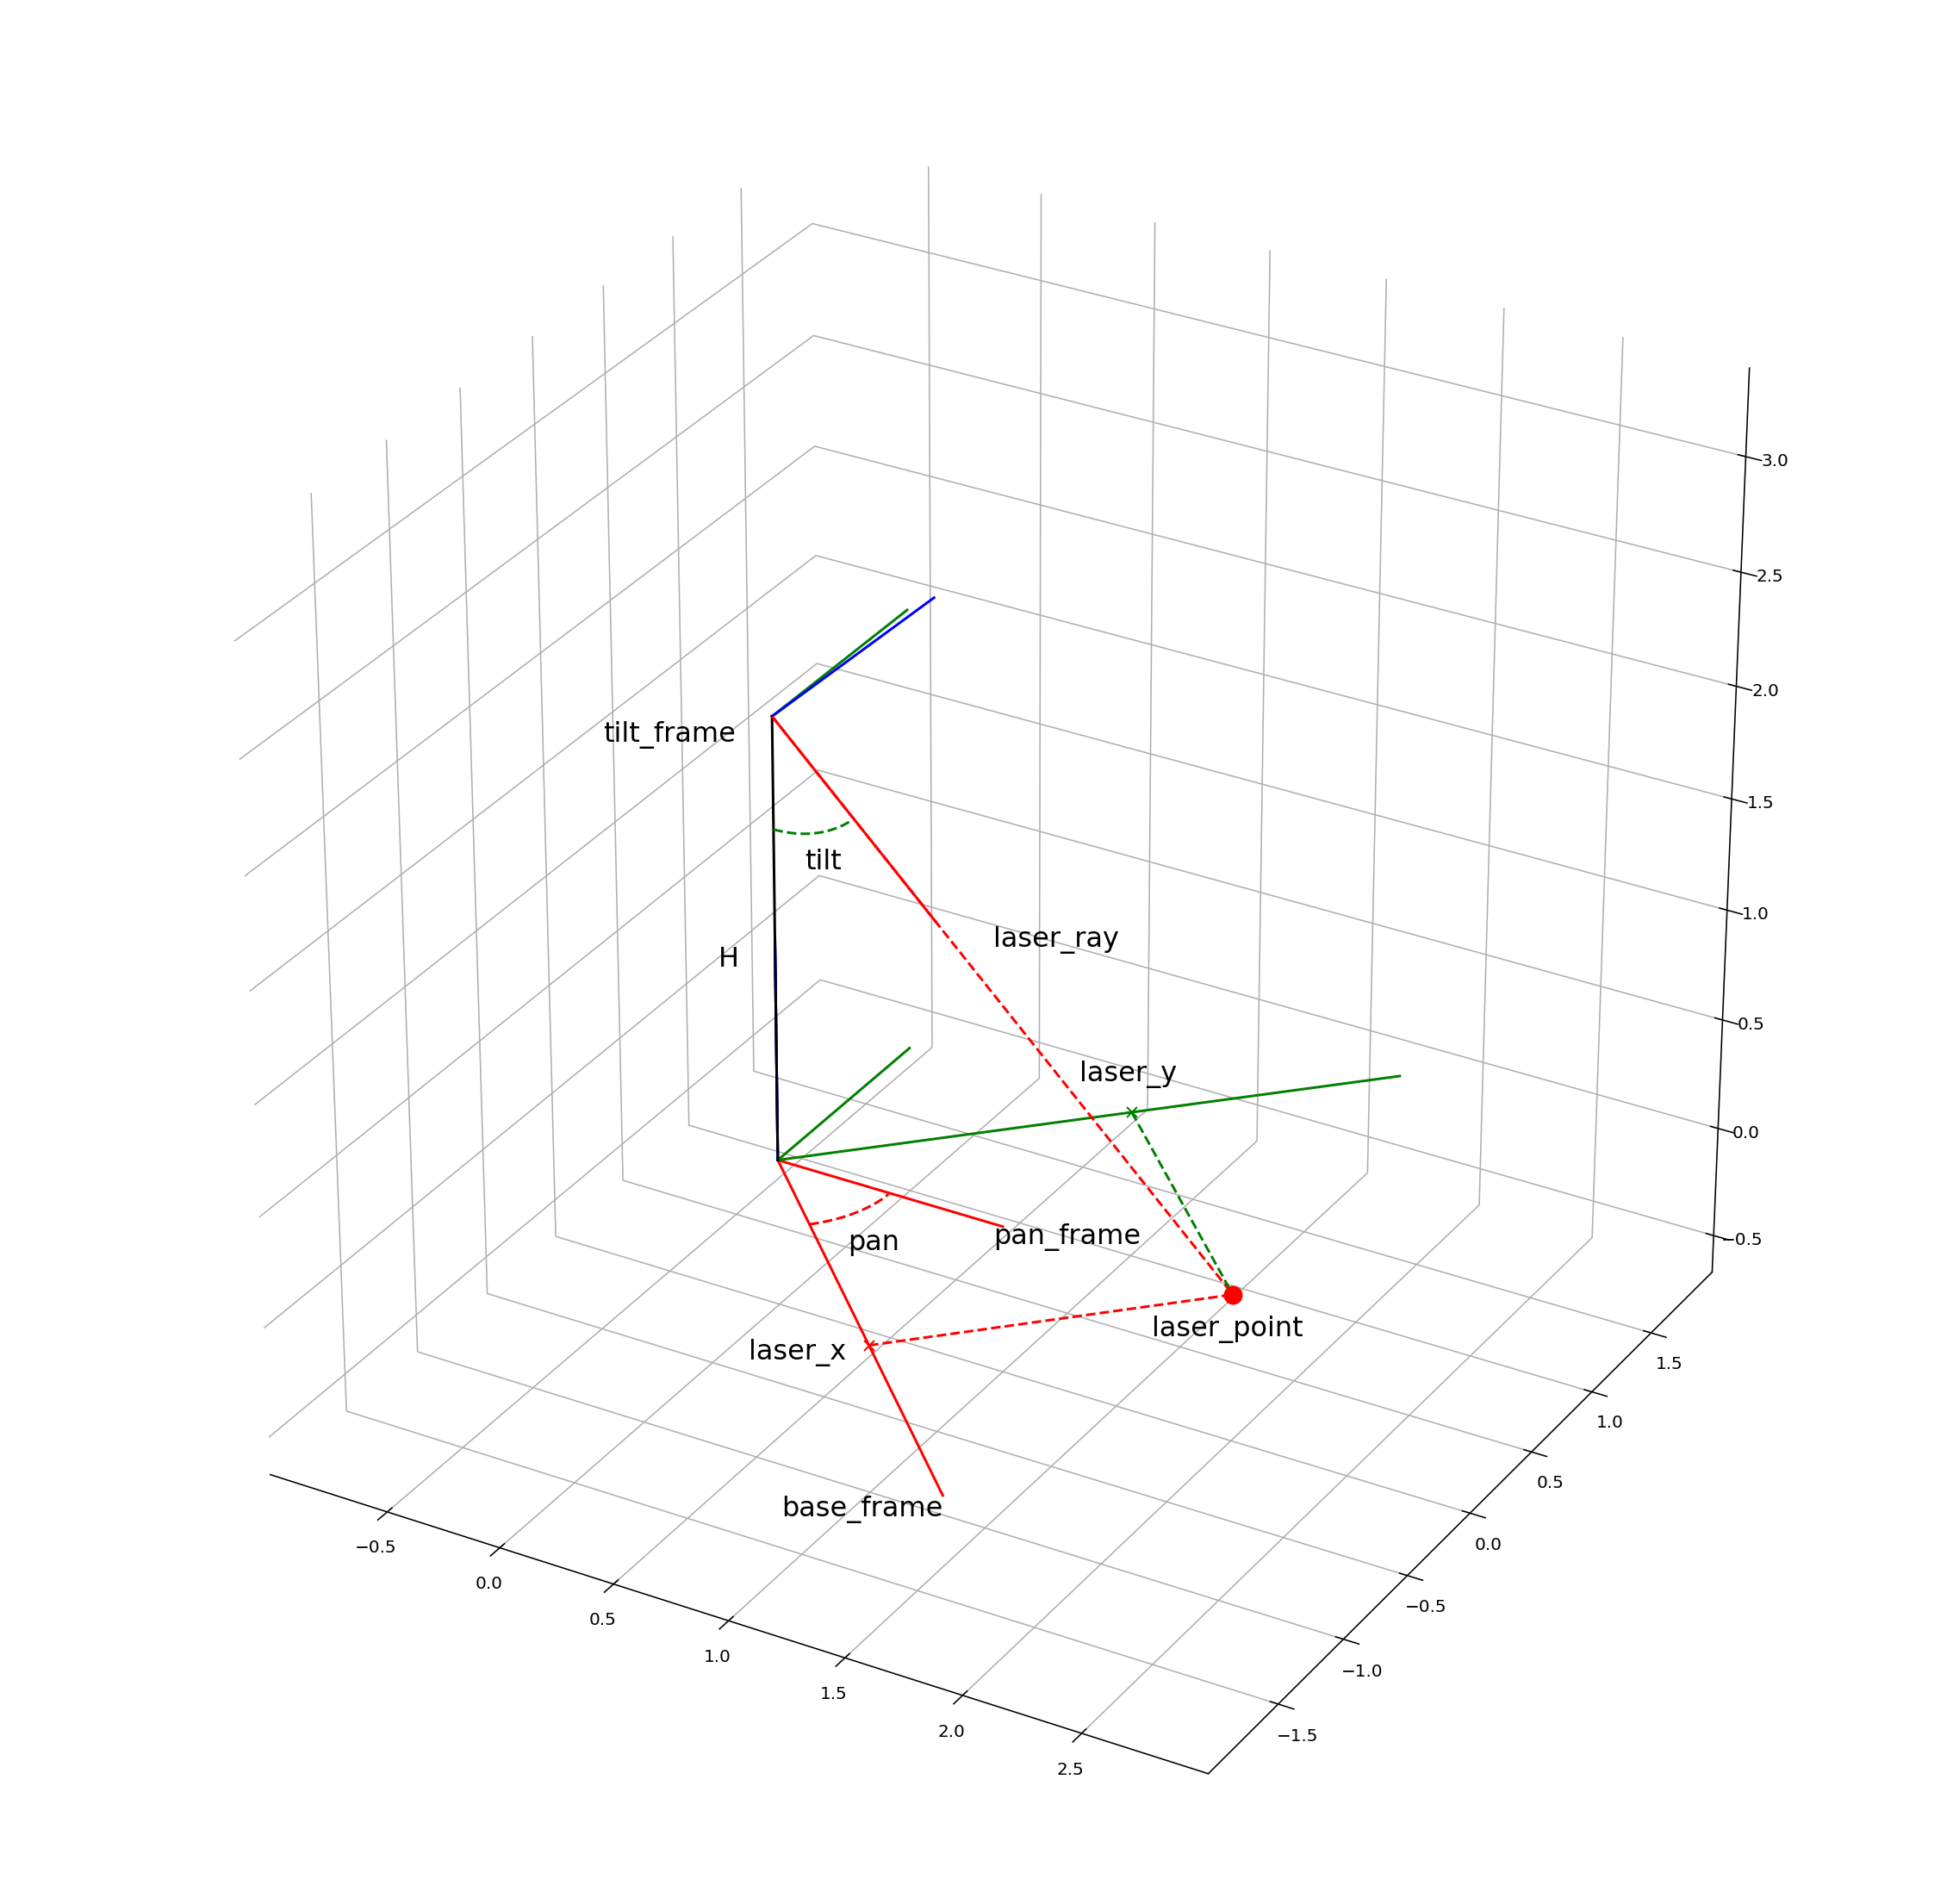
\includegraphics[width=\textwidth]{img/model1XY.png}%
	\caption{First Model, Pan \& Tilt Angle}
	\label{fig:firstModelPanTilt}
\end{figure}
\subsubsection{Inverse Kinematic}
The inverse kinematic takes as input the triple (\textit{x, y, z}) of the laser point and returns the corresponding \textbf{pan} and \textbf{tilt} angles.\\
In addition to \ref{eq:d}, we can say that:
\begin{align}
    H-z =& D\by\cos(tilt)\\
	L =& D\by\sin(tilt) \label{eq:dsin}\\
	L=& \sqrt{x^2+y^2}
\end{align}
Thus, we have that:
\begin{align}
    tilt =& \arctan\bigg(\frac{L}{H-z}\bigg) \label{eq:tiltik}\\
\end{align}
Finally, thanks to equations \ref{eq:x} and \ref{eq:y} we can immediately obtain:
\begin{align}
	pan=& \arctan\bigg(\frac{y}{x}\bigg)\label{eq:panik}
\end{align}
\\
\subsection{Second Model}
The second model is slightly different from the first, as we can see in figure \ref{fig:secondModelRefFrame}. In that case, we have the laser ray which is perpendicular to the x axis of the \textbf{tilt\_frame}. One could think that to solve the inverse kinematic, adding 90 degrees to the tilt angle could be enough. However, since the ray origin does not coincide with the origin of the frame, this is wrong. Changing the tilt angle will not change only the direction of the ray, but also the position of its origin. This makes the kinematic a bit more complicated for that model.
\\
Here we report only the inverse kinematic as it is the most interesting to understand. Note that the assumption made for the \textit{z} of the laser point in section \ref{subs:firstModel} still holds.

\begin{figure}
	\centering
	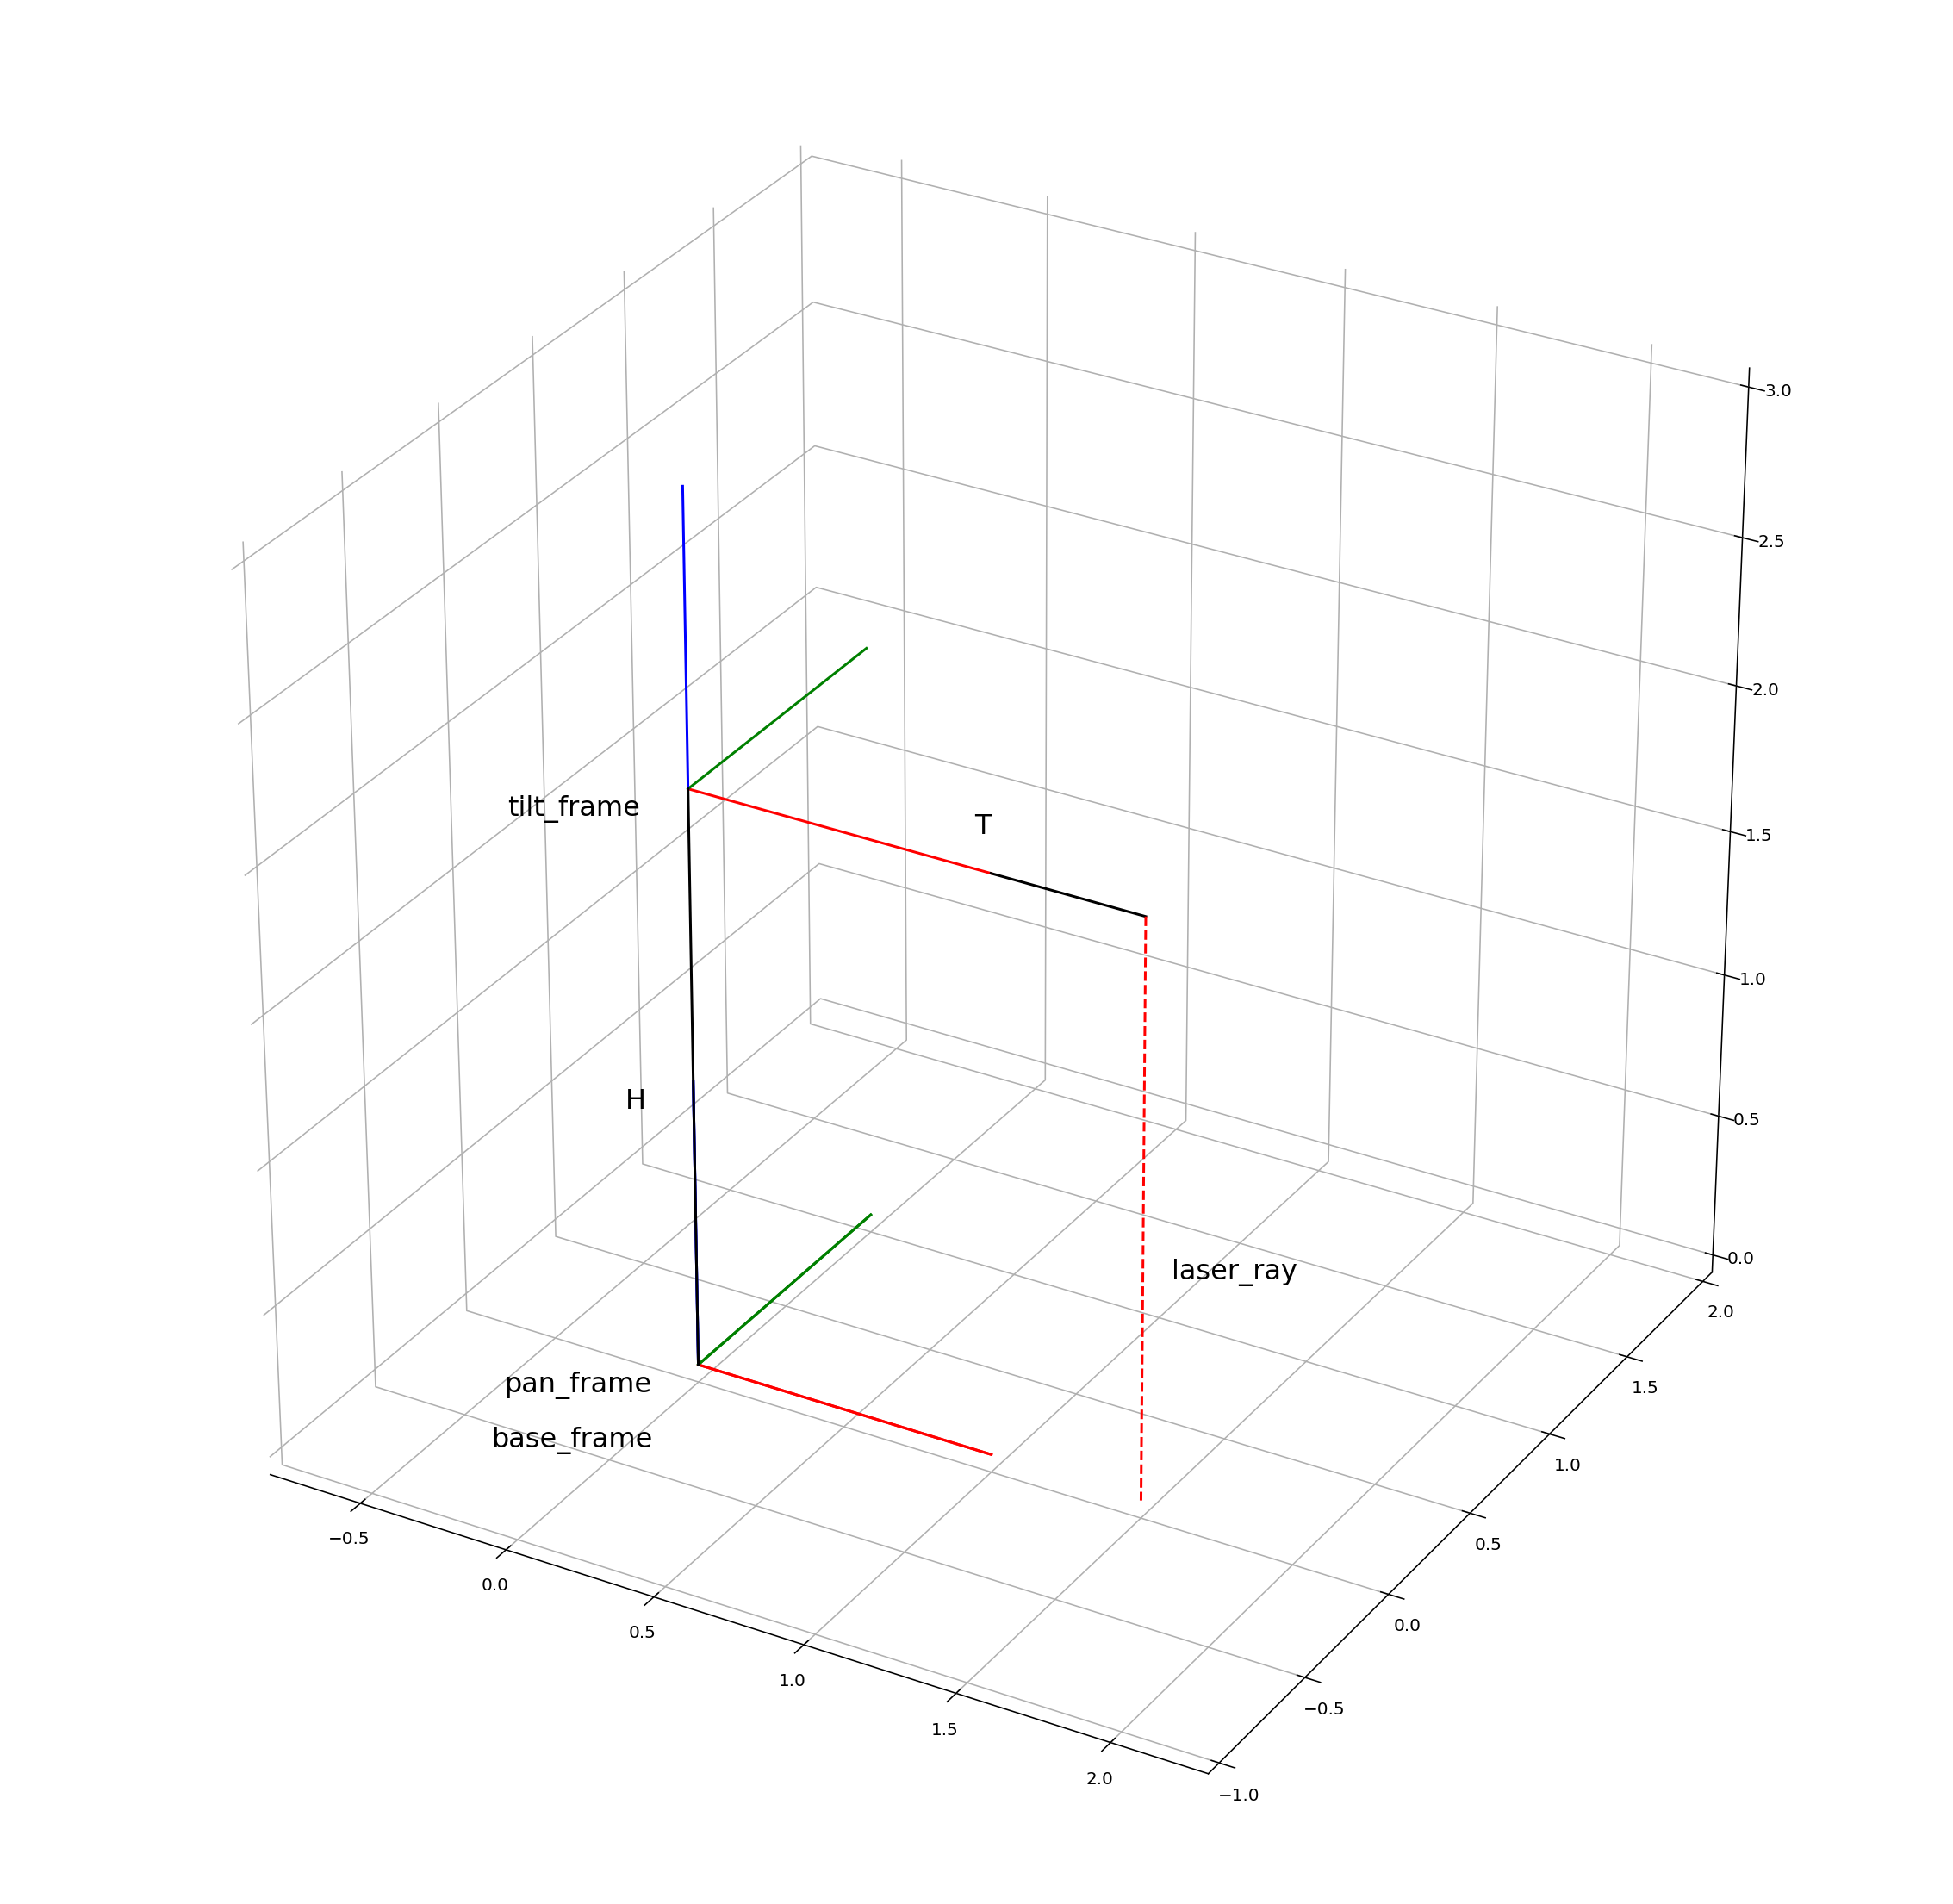
\includegraphics[width=\textwidth]{img/secondModel.png}%
	\caption{Second Model, Reference Frames}
	\label{fig:secondModelRefFrame}
\end{figure}

\subsubsection{Inverse Kinematic}
\begin{figure}
	\centering
	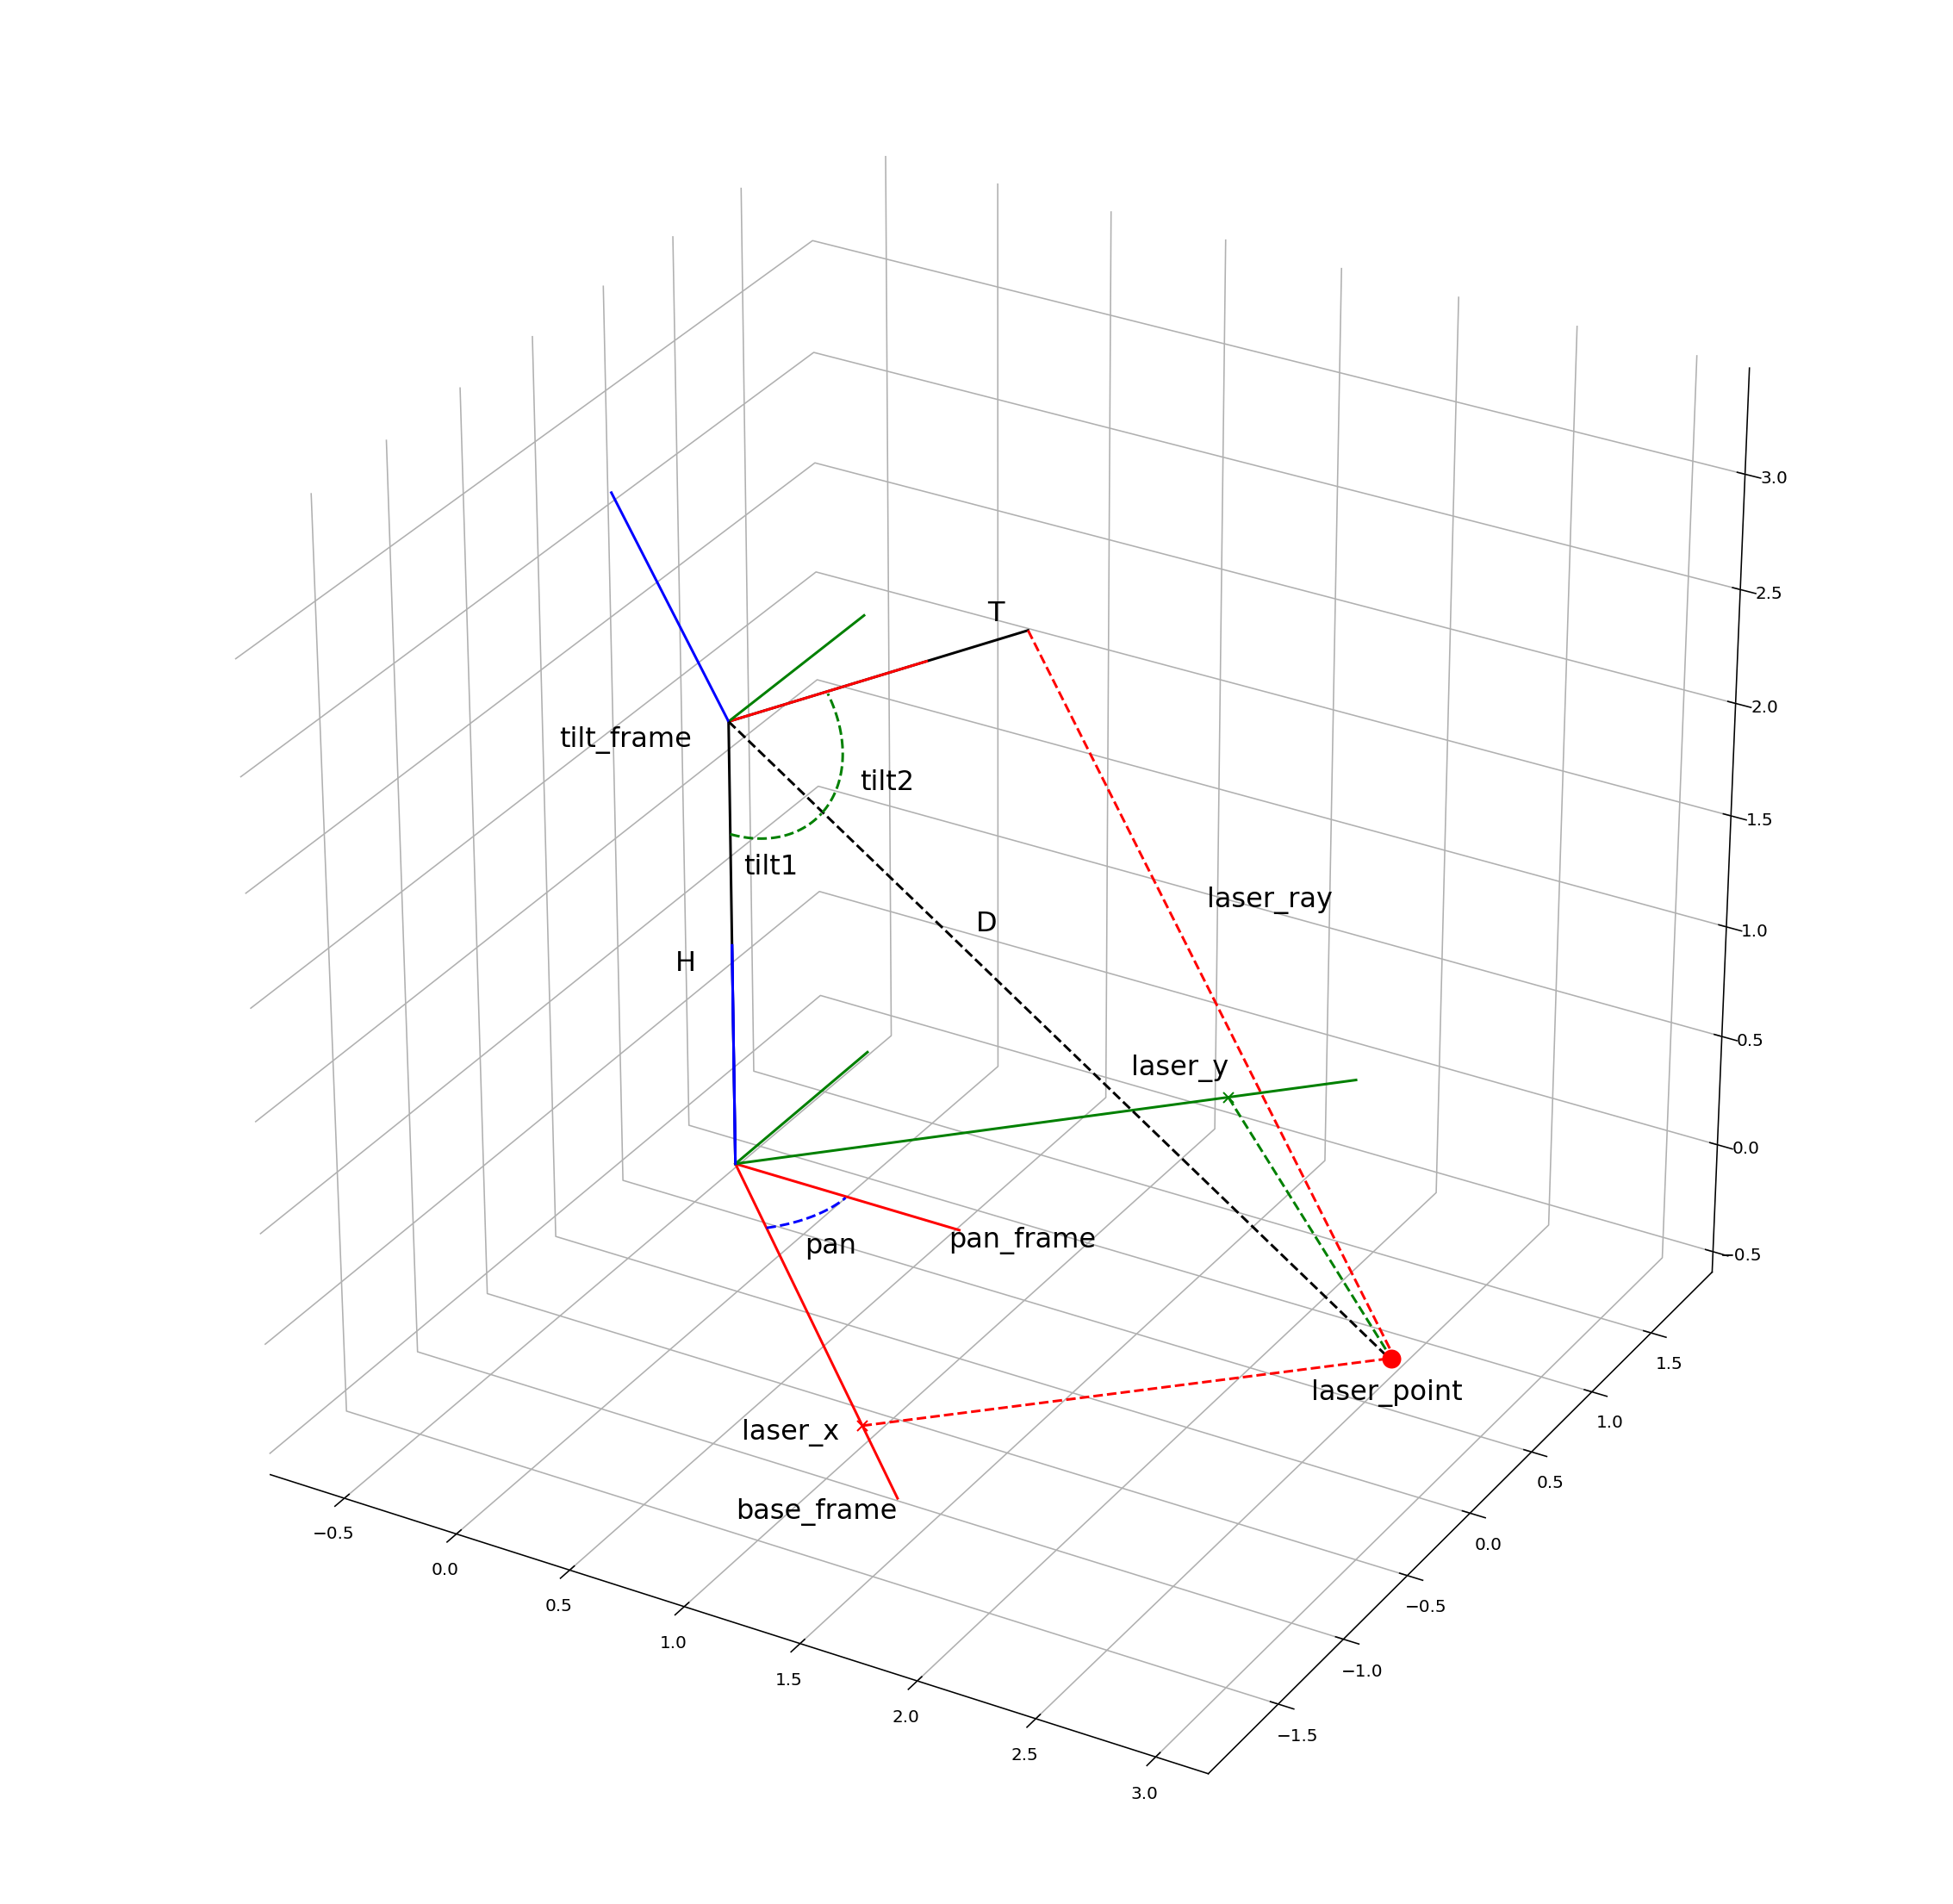
\includegraphics[width=\textwidth]{img/model2XY.png}%
	\caption{Second Model, Pan \& Tilt}
	\label{fig:secondModelPanTilt}
\end{figure}
First, we recall \textbf{L}, \textbf{D} and we introduce \textbf{T}:
\begin{itemize}
    \item \textbf{L} as the distance from the \textbf{pan\_frame} origin to the projection of the laser point on the \textbf{base\_frame};
    \item \textbf{D} as the distance from the \textbf{tilt\_frame} origin to the laser point;
    \item \textbf{T} as the known distance from the \textbf{tilt\_frame} origin to the laser ray origin.
\end{itemize}
As we can see in figure \ref{fig:secondModelPanTilt}, we have to decompose \textbf{tilt} in two parts, this is why we explicitly draw \textbf{D} that time. On the contrary, \textbf{pan} is obtained in the same way we did for the first model, thus:
\begin{align}
	pan=& \arctan\bigg(\frac{y}{x}\bigg)\label{eq:panik2}
\end{align}
Then we compute \textbf{L} and \textbf{D}:
\begin{align}
	L=& \sqrt{x^2+y^2}\\
	D=& \sqrt{(H-z)^2 + L^2}
\end{align}
Finally,
\begin{align}
	tilt1 =& \arcatn\bigg(\frac{L}{H-z}\bigg)\\
	tilt2 =& \arctan\bigg(\frac{D}{T}\bigg)\\
	tilt =& tilt1 + tilt2
\end{align}
\\
\section{Human Pointing Model}
The approach we follow to model human pointing is the one used in \cite{gromov2018robot}. The head-finger model defines human pointing rays as originating at a centroid of the head and passing through the index fingertip. 

\chapter{Hardware Implementation}
\label{chap:2}
In this chapter we describe the hardware implementation of the system. In particular, in section \ref{sec:turret12} and \ref{sec:turret64} we will focus on the two different laser turrets built, pointing out all the issues and differences that make the second one better. We also mention the arm IMU device and the groud robot used for reconstruct human pointing and build our demos respectively.
\section{First Turret Model} \label{sec:turret12}
Figures \ref{fig:model1Photo} shows the first turret. As we can better see in figure \ref{fig:model13D} and \ref{fig:model13DCap}, it follows the model already seen in chapter \ref{chap:1}. So, at the base we have one servo motor in charge to control the \emph{pan} angle. On its flange, a second motor is mounted with a plastic bracket on its own flange. The laser diode is then mounted in the middle of that bracket, in such a way that its direction passes through the middle of the servo shaft. So, the second servo directly controls the \emph{tilt} angle. 
The \emph{Arduino Uno Board} and the \emph{Bioloid Bus Serial Interface} conclude our hardware list.
\\In the next sections we analyze each parts and their uses in details.
\begin{figure}
	\centering
	\includegraphics[width=\textwidth]{img/model1Photo.png}%
	\caption{First Turret Model, Actual Photos}
	\label{fig:model1Photo}
\end{figure}
\begin{figure}
	\centering
	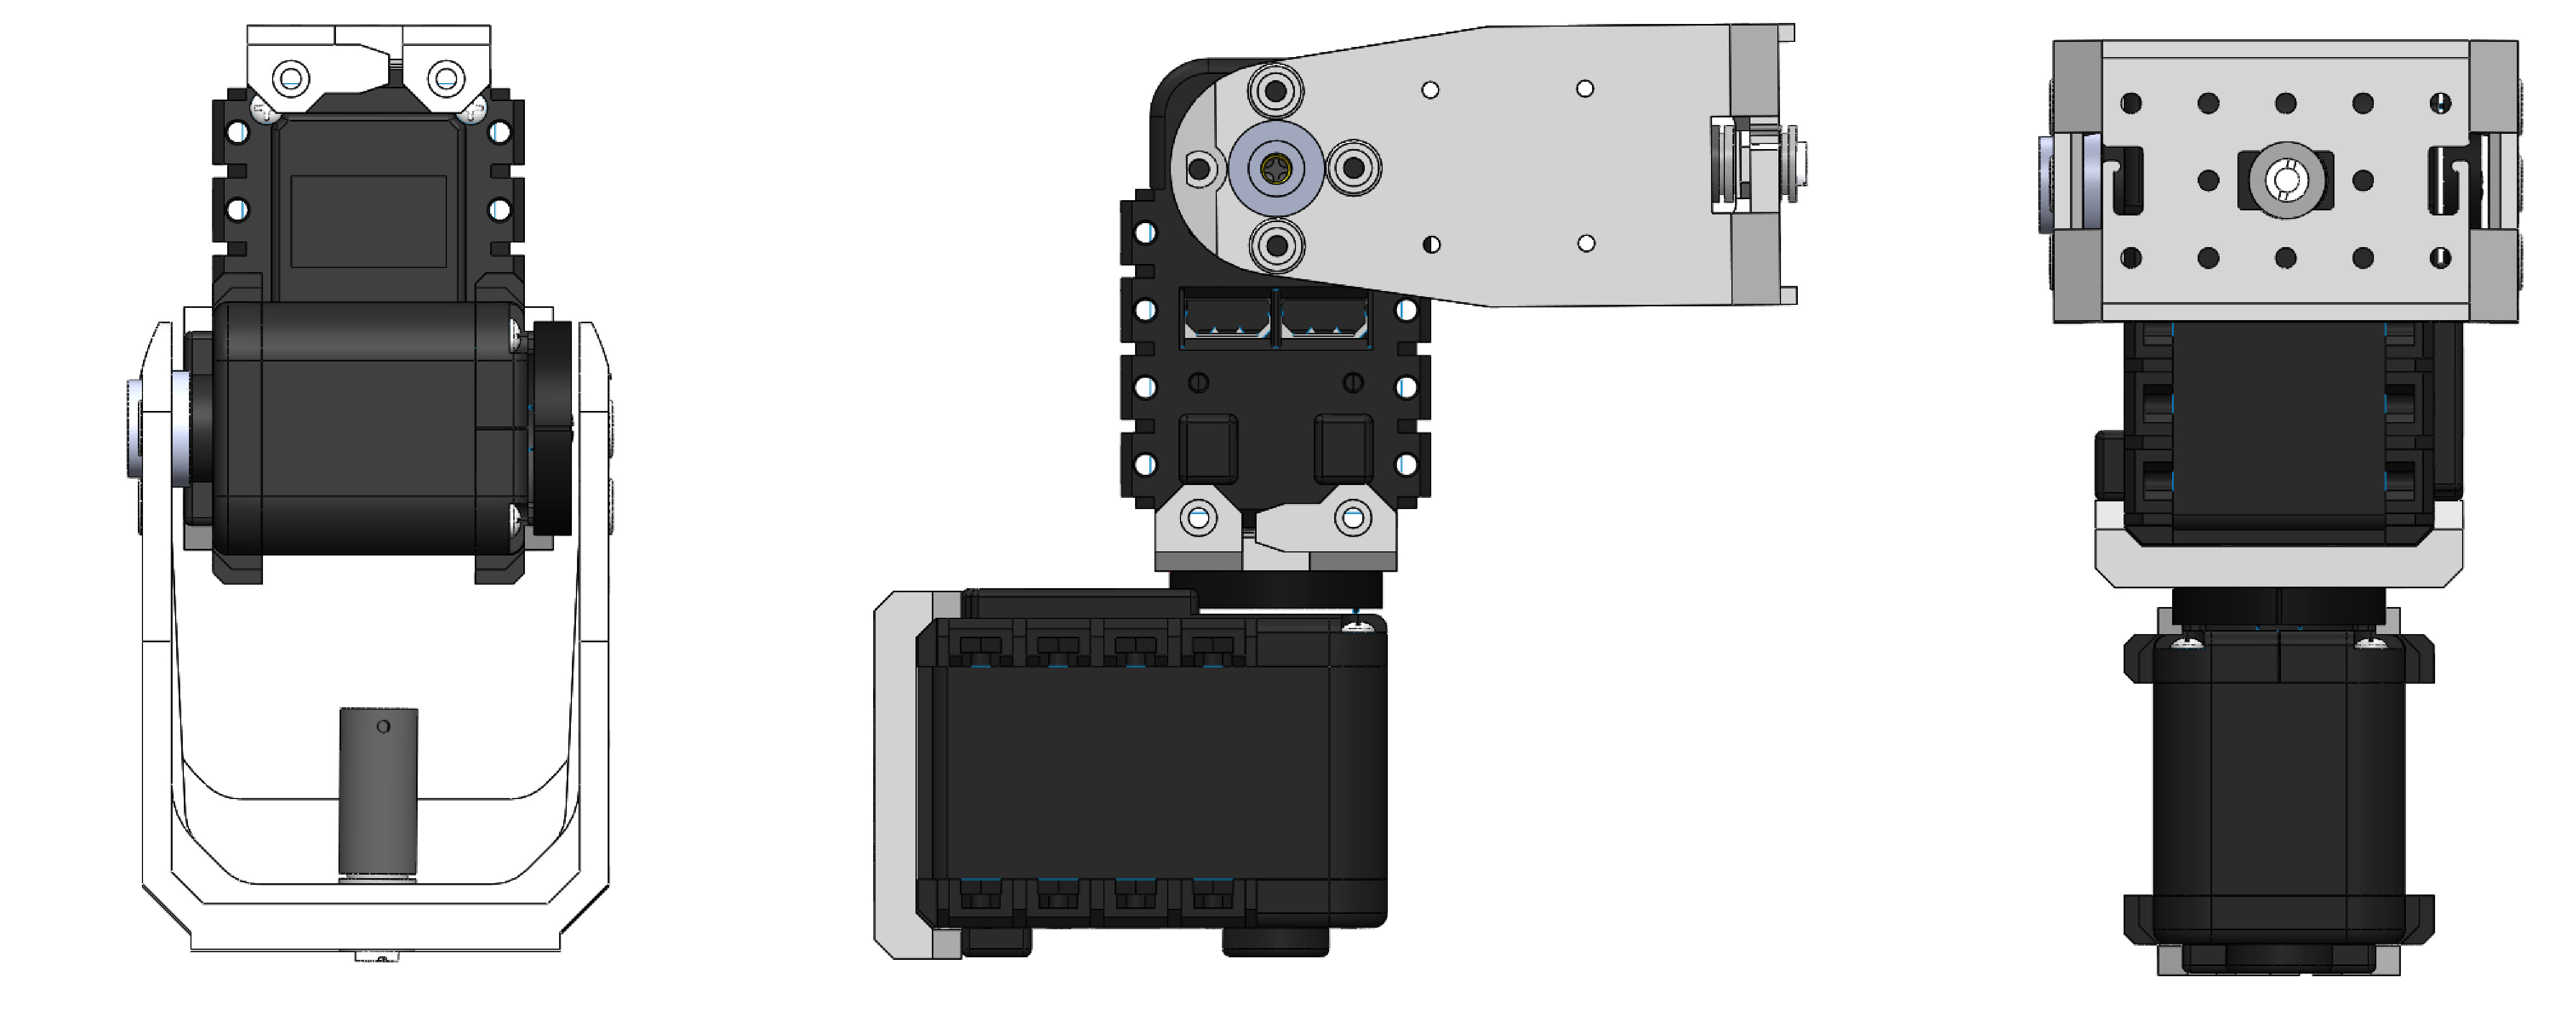
\includegraphics[width=\textwidth]{img/model13dsides.png}%
	\caption{First Turret Modelm 3D from Different Views}
	\label{fig:model13D}
\end{figure}
\begin{figure}
	\centering
	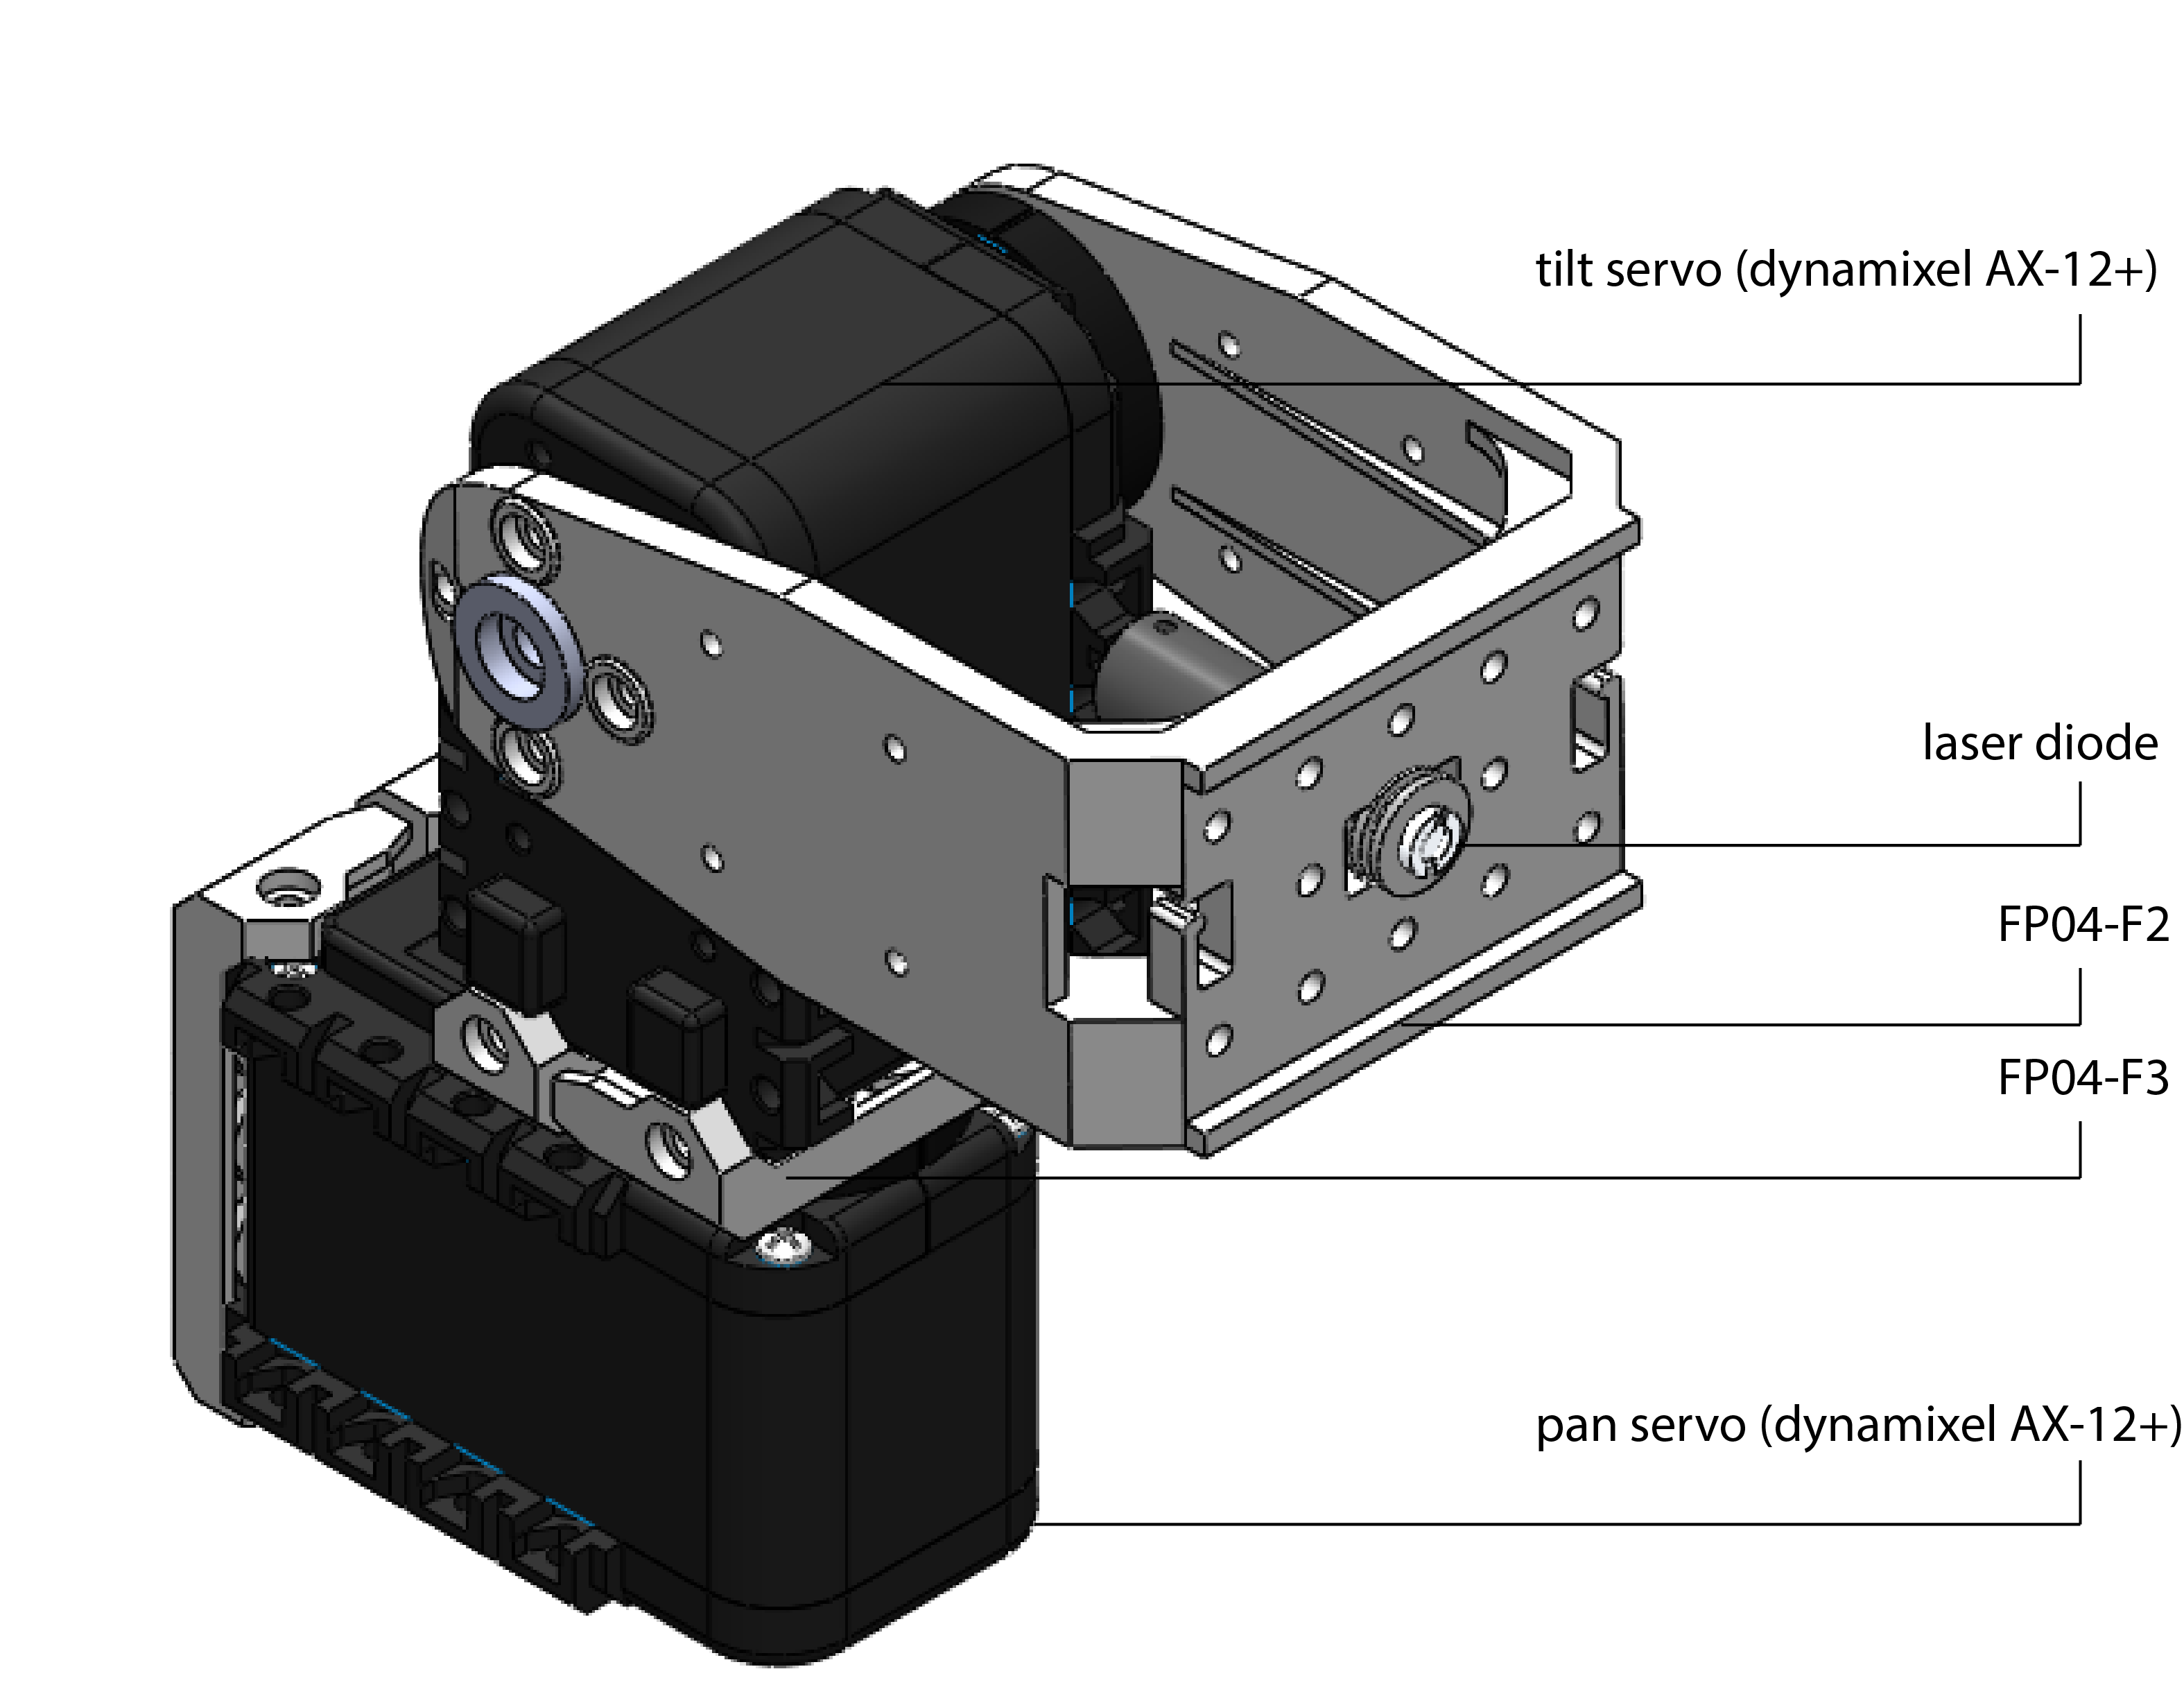
\includegraphics[width=\textwidth]{img/model13dCap.png}%
	\caption{First Turret Model, 3D with Parts Names}
	\label{fig:model13DCap}
\end{figure}
\subsection{Dynamixel AX-12+}
As reported on the official website \cite{web-AX-12}:\\ \virgolette{\emph{the DYNAMIXEL is a smart actuator system developed to be the exclusive connecting joints on a robot or mechanical structure. DYNAMIXELS’ are designed to be modular and daisy chained on any robot or mechanical design for powerful and flexible robotic movements. The DYNAMIXEL is a high performance actuator with a fully integrated DC (Direct Current) Motor + Reduction Gearhead + Controller + Driver + Network, all in one servo module actuator. Programmable and networkable, actuator status can be read and monitored through a data packet stream.}}\\
The first turret is composed of two \textbf{Dynamixel AX-12+} motors.
\clearpage
\subsection{Motor Specification}
The full datasheet can be found here \cite{datasheet-AX-12}. We are mostly interested in two specifications: 
\begin{itemize}
    \item \textbf{Resolution}: $0.29^{\circ}$;
    \item \textbf{Communication speed}: 7343 bps $\sim$ 1 Mbps.
\end{itemize}
Those are the values that set the limitations for that turret, causing the issues we discuss in the next section.
\begin{figure}
	\centering
	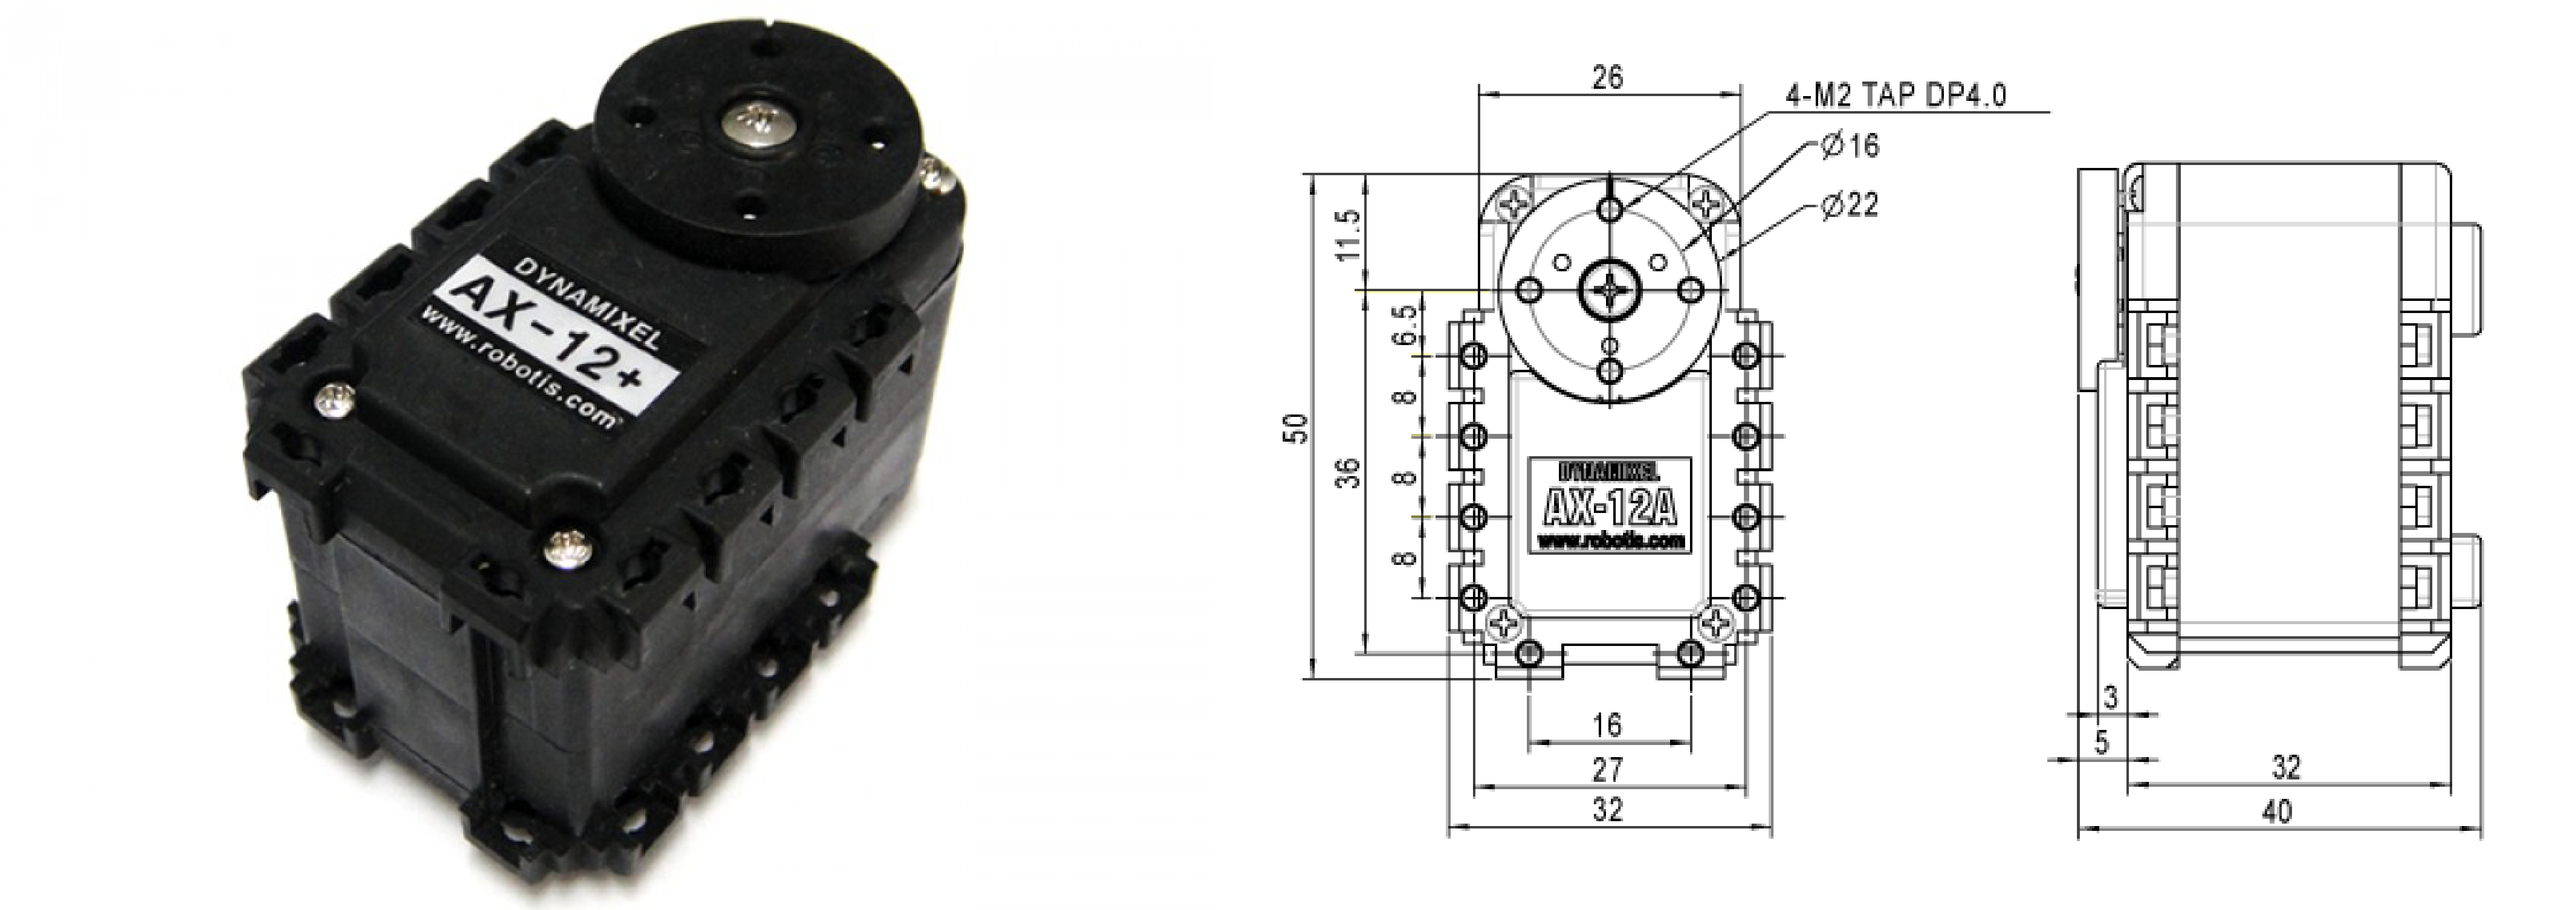
\includegraphics[width=\textwidth]{img/ax12+.png}%
	\caption{Dynamixel AX-12+}
	\label{fig:ax12+}
\end{figure}
\subsection{Issues}\label{subs:firstModel:issues}
Here we will only report the issues raised by the motors. Solutions are discussed in the next chapter.
\subsubsection{Servo Resolution and Slow Speed Limit}
Even though a resolution of $0.29^{\circ}$ could seem pretty good, that value heavily limits the performance of the turret. As a matter of fact, in our system, the joint will be often asked to do very small movement and, thus, drawing tiny angles. Moreover, the motor is not able to move with too much low speed values. That issue becomes even bigger when the laser dot moves far from the turret: the angles become always more smaller. The result is that the performances of the turret can be good enough only on a small size space around the turret, but that is not certainly enough for our system.
\subsubsection{Trajectory Smoothness}
The performances degradation heavily impacts the smoothness of trajectory of the laser dot. Playing with servos internal parameters we could try to find the right trade-off between precision and smoothness, but since the relative localization is based on the laser positions and the user following those positions, then we can not sacrifice too much either precision or smoothness.
\subsubsection{Slow Communication Protocol}
This is the main issue. It is only partially related with the communication speed of the motors. Of course, with a higher speed, we could afford to use a slower protocol. Anyway, solving that issue allows us to obtain the best from that turret, hitting its limits, but obtaining a system which could work well enough for our purposes. Since the solution is part of the software implementation, it will be presented in the next chapter.

\subsection{Bioloid Bus Interface}
This board allows PC to communicate with Bioloid bus devices (e.g. Dynamixel AX-12) using a USB cable at speeds of up to 1.0 Mbps. In other words,
this simple device provides serial communication between the PC and the motors. It is also needed to provide voltage to the motors. We can not use it to power up the laser as the output voltage is too high and there is no voltage regulator.
\begin{figure}[h]
	\centering
	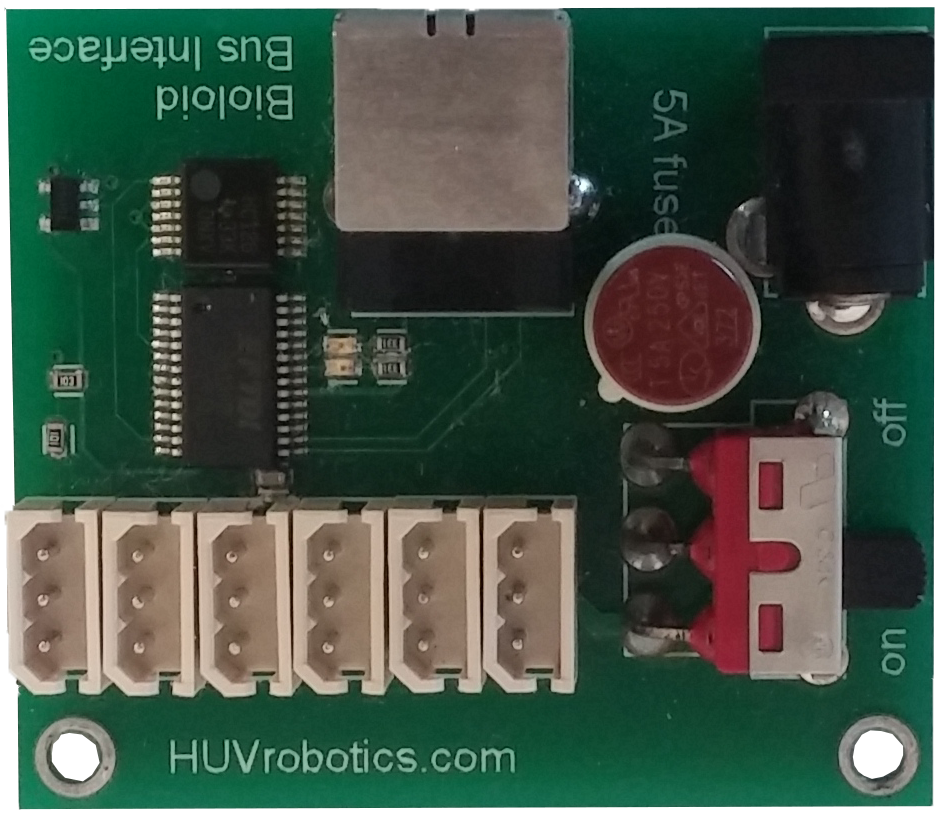
\includegraphics[width=.5\textwidth]{img/bioloid.png}%
	\caption{Bioloid Bus Interface}
	\label{fig:busInterface}
\end{figure}
\subsection{Laser Diode and Arduino Uno Board}
We use a simple 5V red laser diode powered directly from an \emph{Arduino Uno Board}. We use that board because it provides a 5V output and thus is a simple and fast solution to power up the laser.
\begin{figure}
\centering
\begin{minipage}{.5\textwidth}
  \centering
  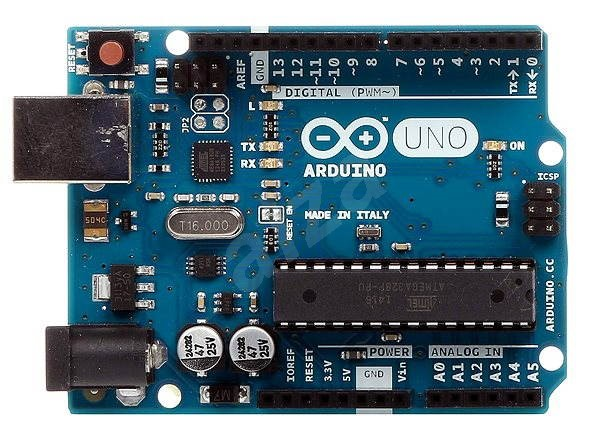
\includegraphics[width=\linewidth]{img/arduino.jpg}
  \captionof{figure}{Arduino Uno Board}
  \label{fig:arduino}
\end{minipage}%
\begin{minipage}{.5\textwidth}
  \centering
  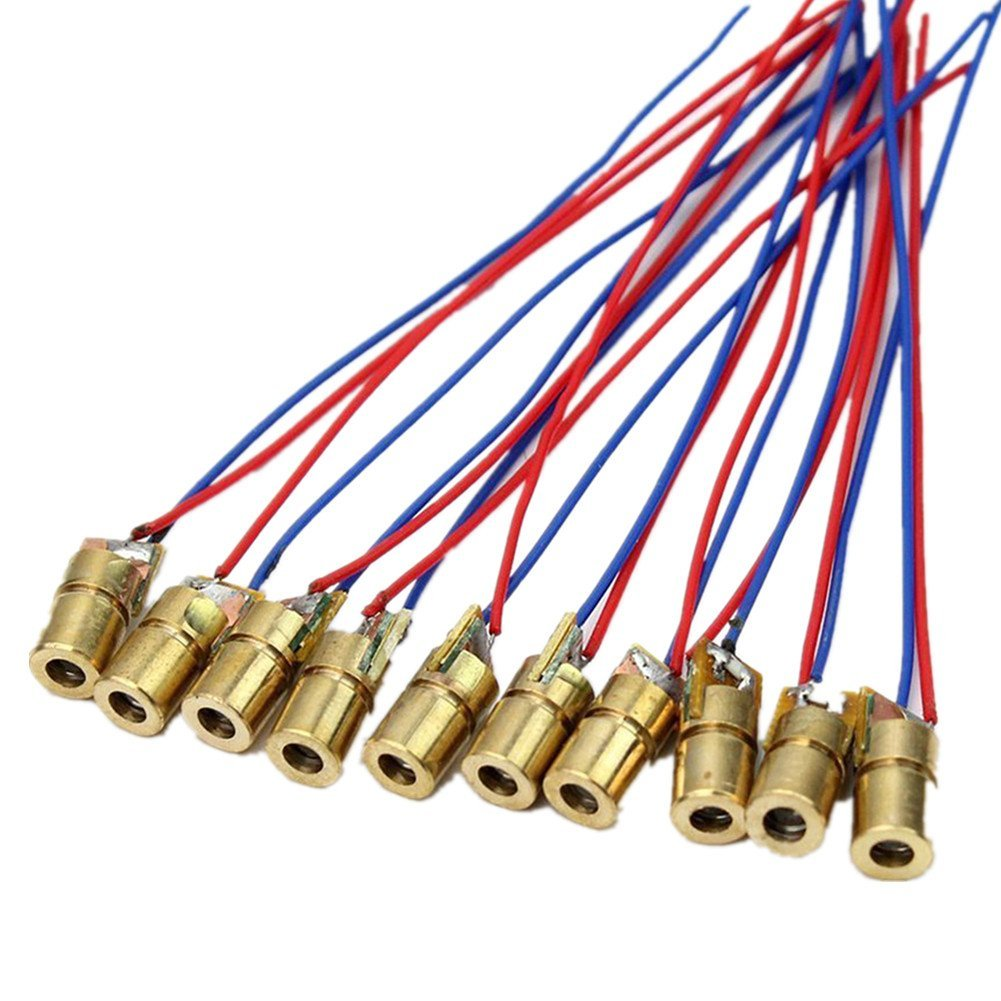
\includegraphics[width=.75\linewidth]{img/diode.jpg}
  \captionof{figure}{Laser Diodes}
  \label{fig:diode}
\end{minipage}
\end{figure}
\clearpage
\subsection{Structural Parts}
Figures \ref{fig:axFrames} shows the plastic frames used to assemble the turret. Mounting instructions can be found in the appendix. \todo{MOVE MOUNTING INSTRUCTIONS TO APPENDIX?}
\begin{figure}
	\centering
	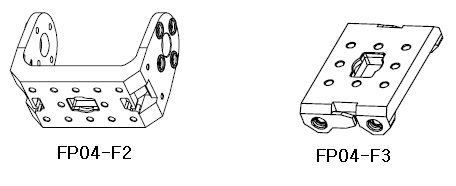
\includegraphics[width=\textwidth]{img/axFrames.png}%
	\caption{Plastic Mounting Frames}
	\label{fig:axFrames}
\end{figure}

\section{Second Turret Model}\label{sec:turret64}
\begin{figure}
	\centering
	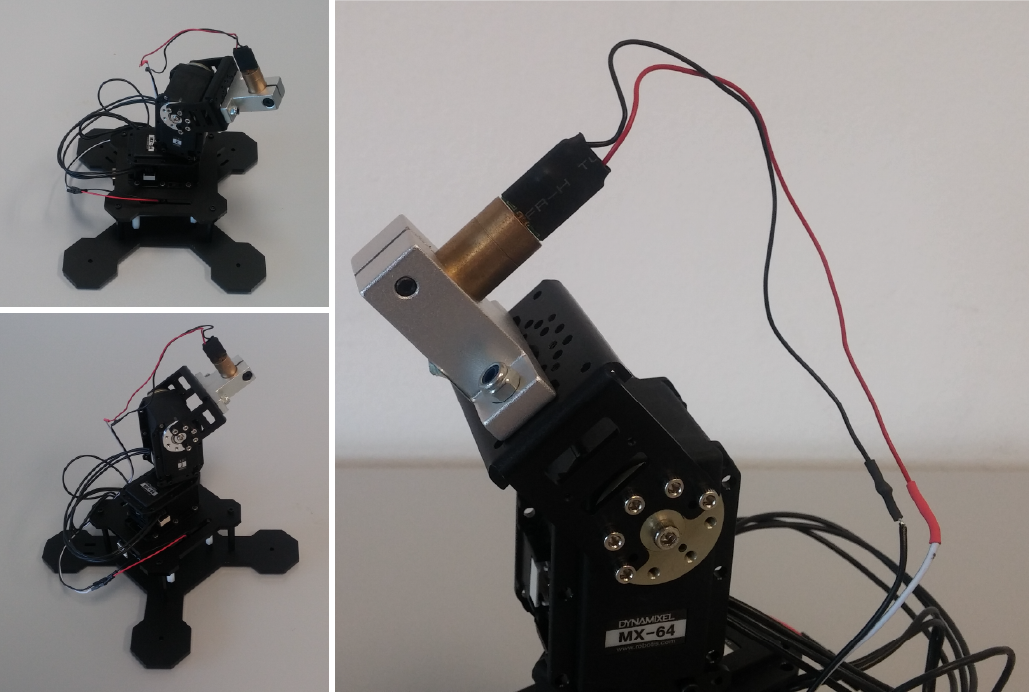
\includegraphics[width=\textwidth]{img/model2Photo.png}%
	\caption{Second Turret Model, Actual Photos}
	\label{fig:model2Photo}
\end{figure}
\begin{figure}
	\centering
	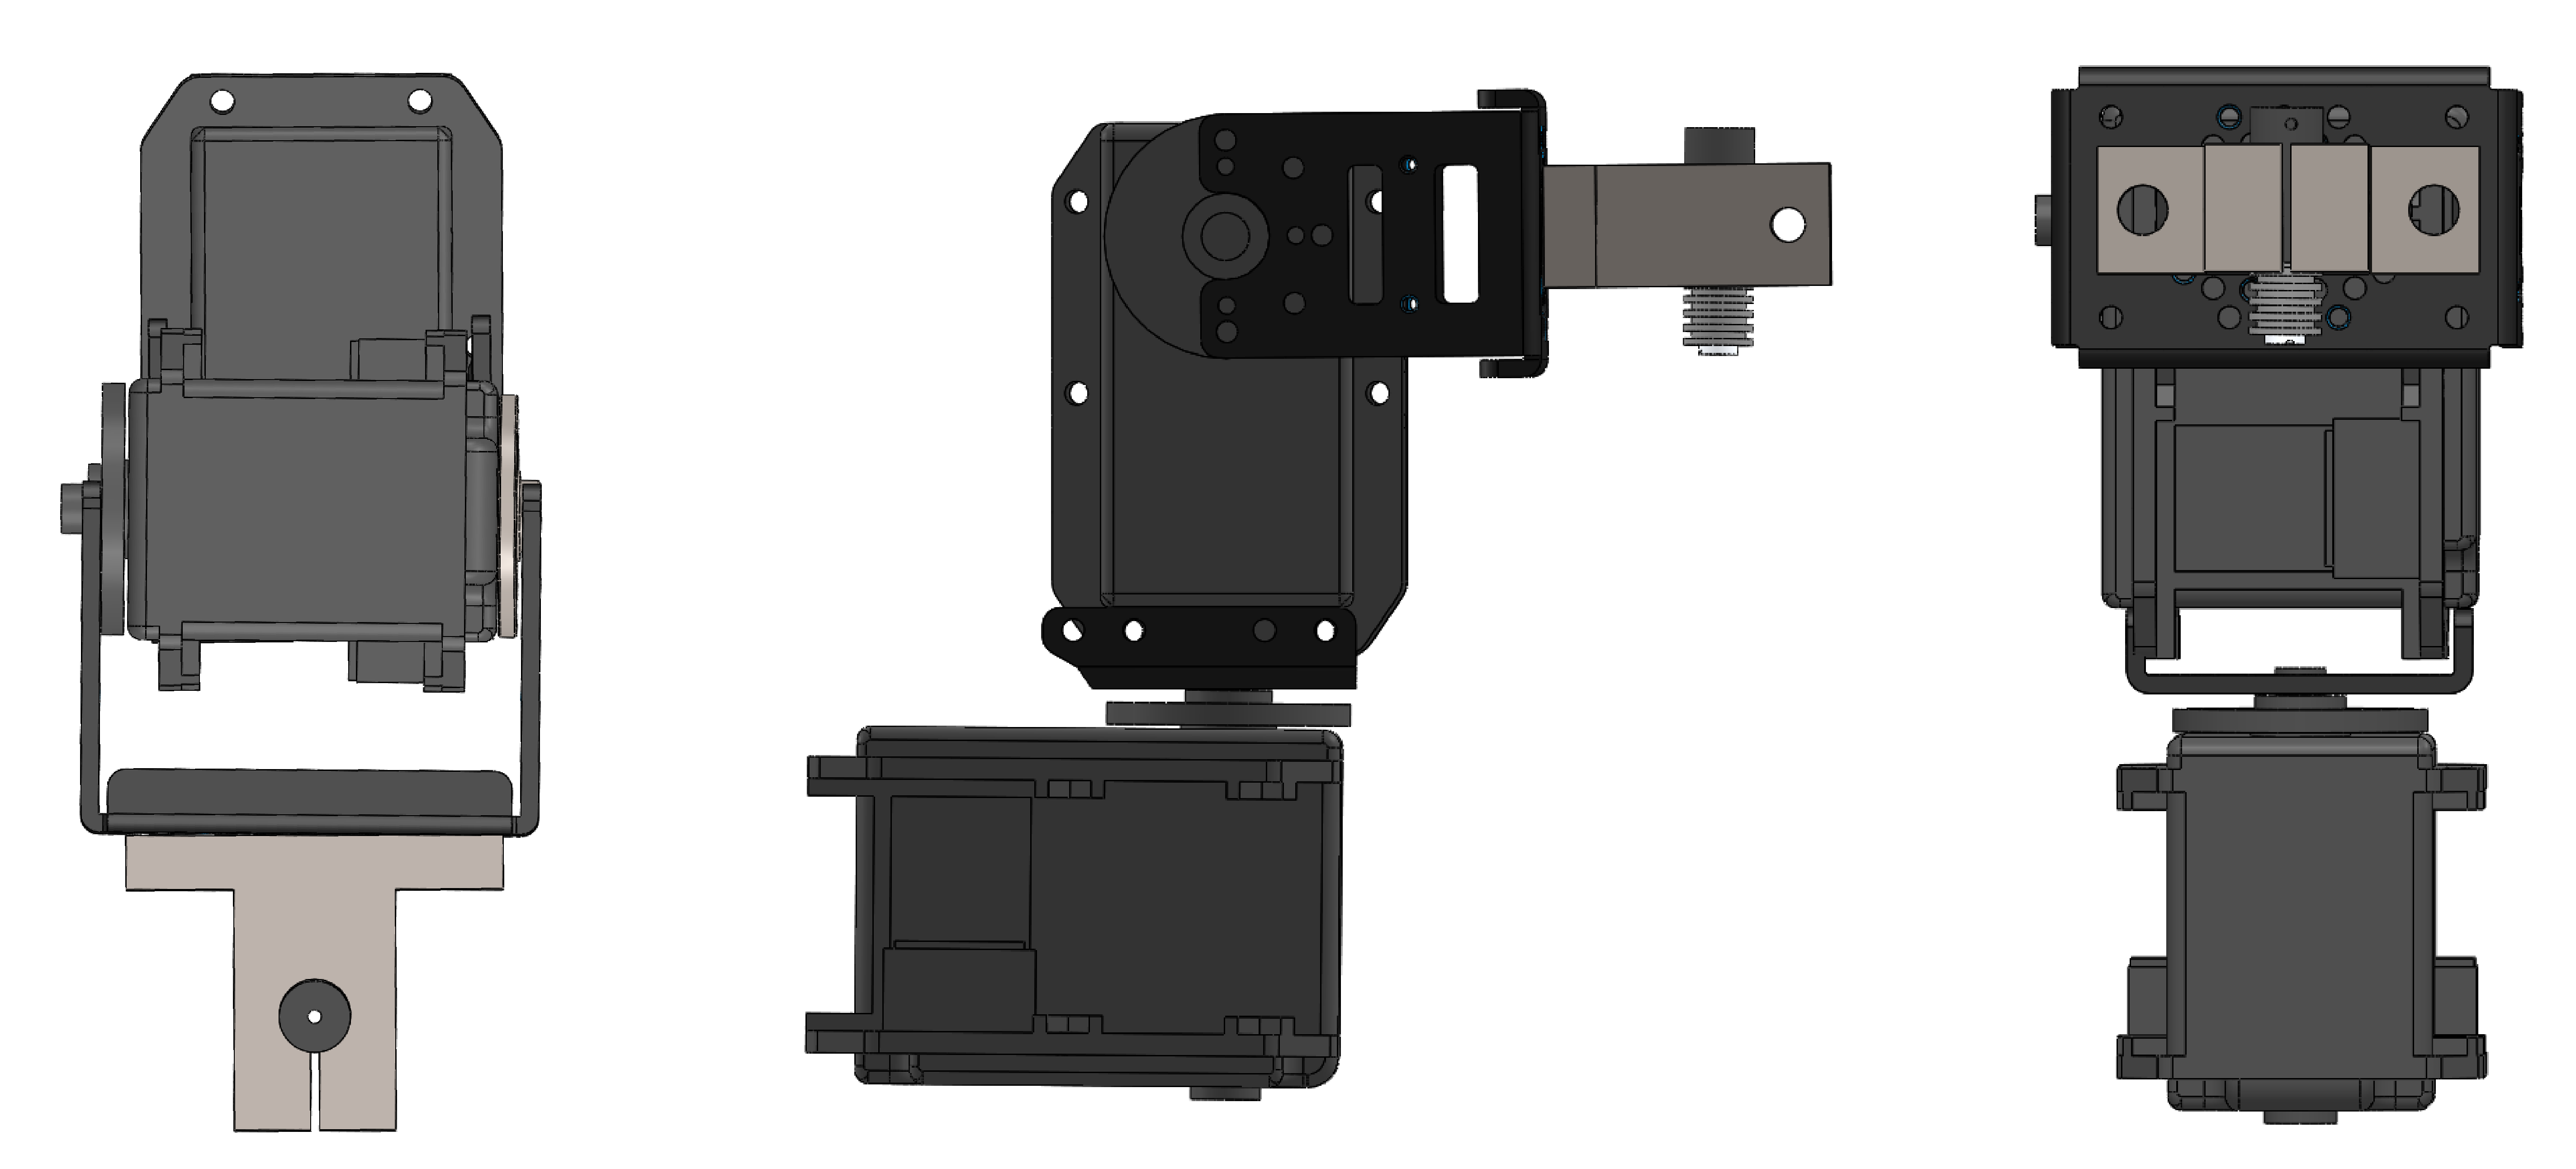
\includegraphics[width=\textwidth]{img/model23dsides.png}%
	\caption{Second Turret Model, 3D from Different Views}
	\label{fig:model23D}
\end{figure}
\begin{figure}
	\centering
	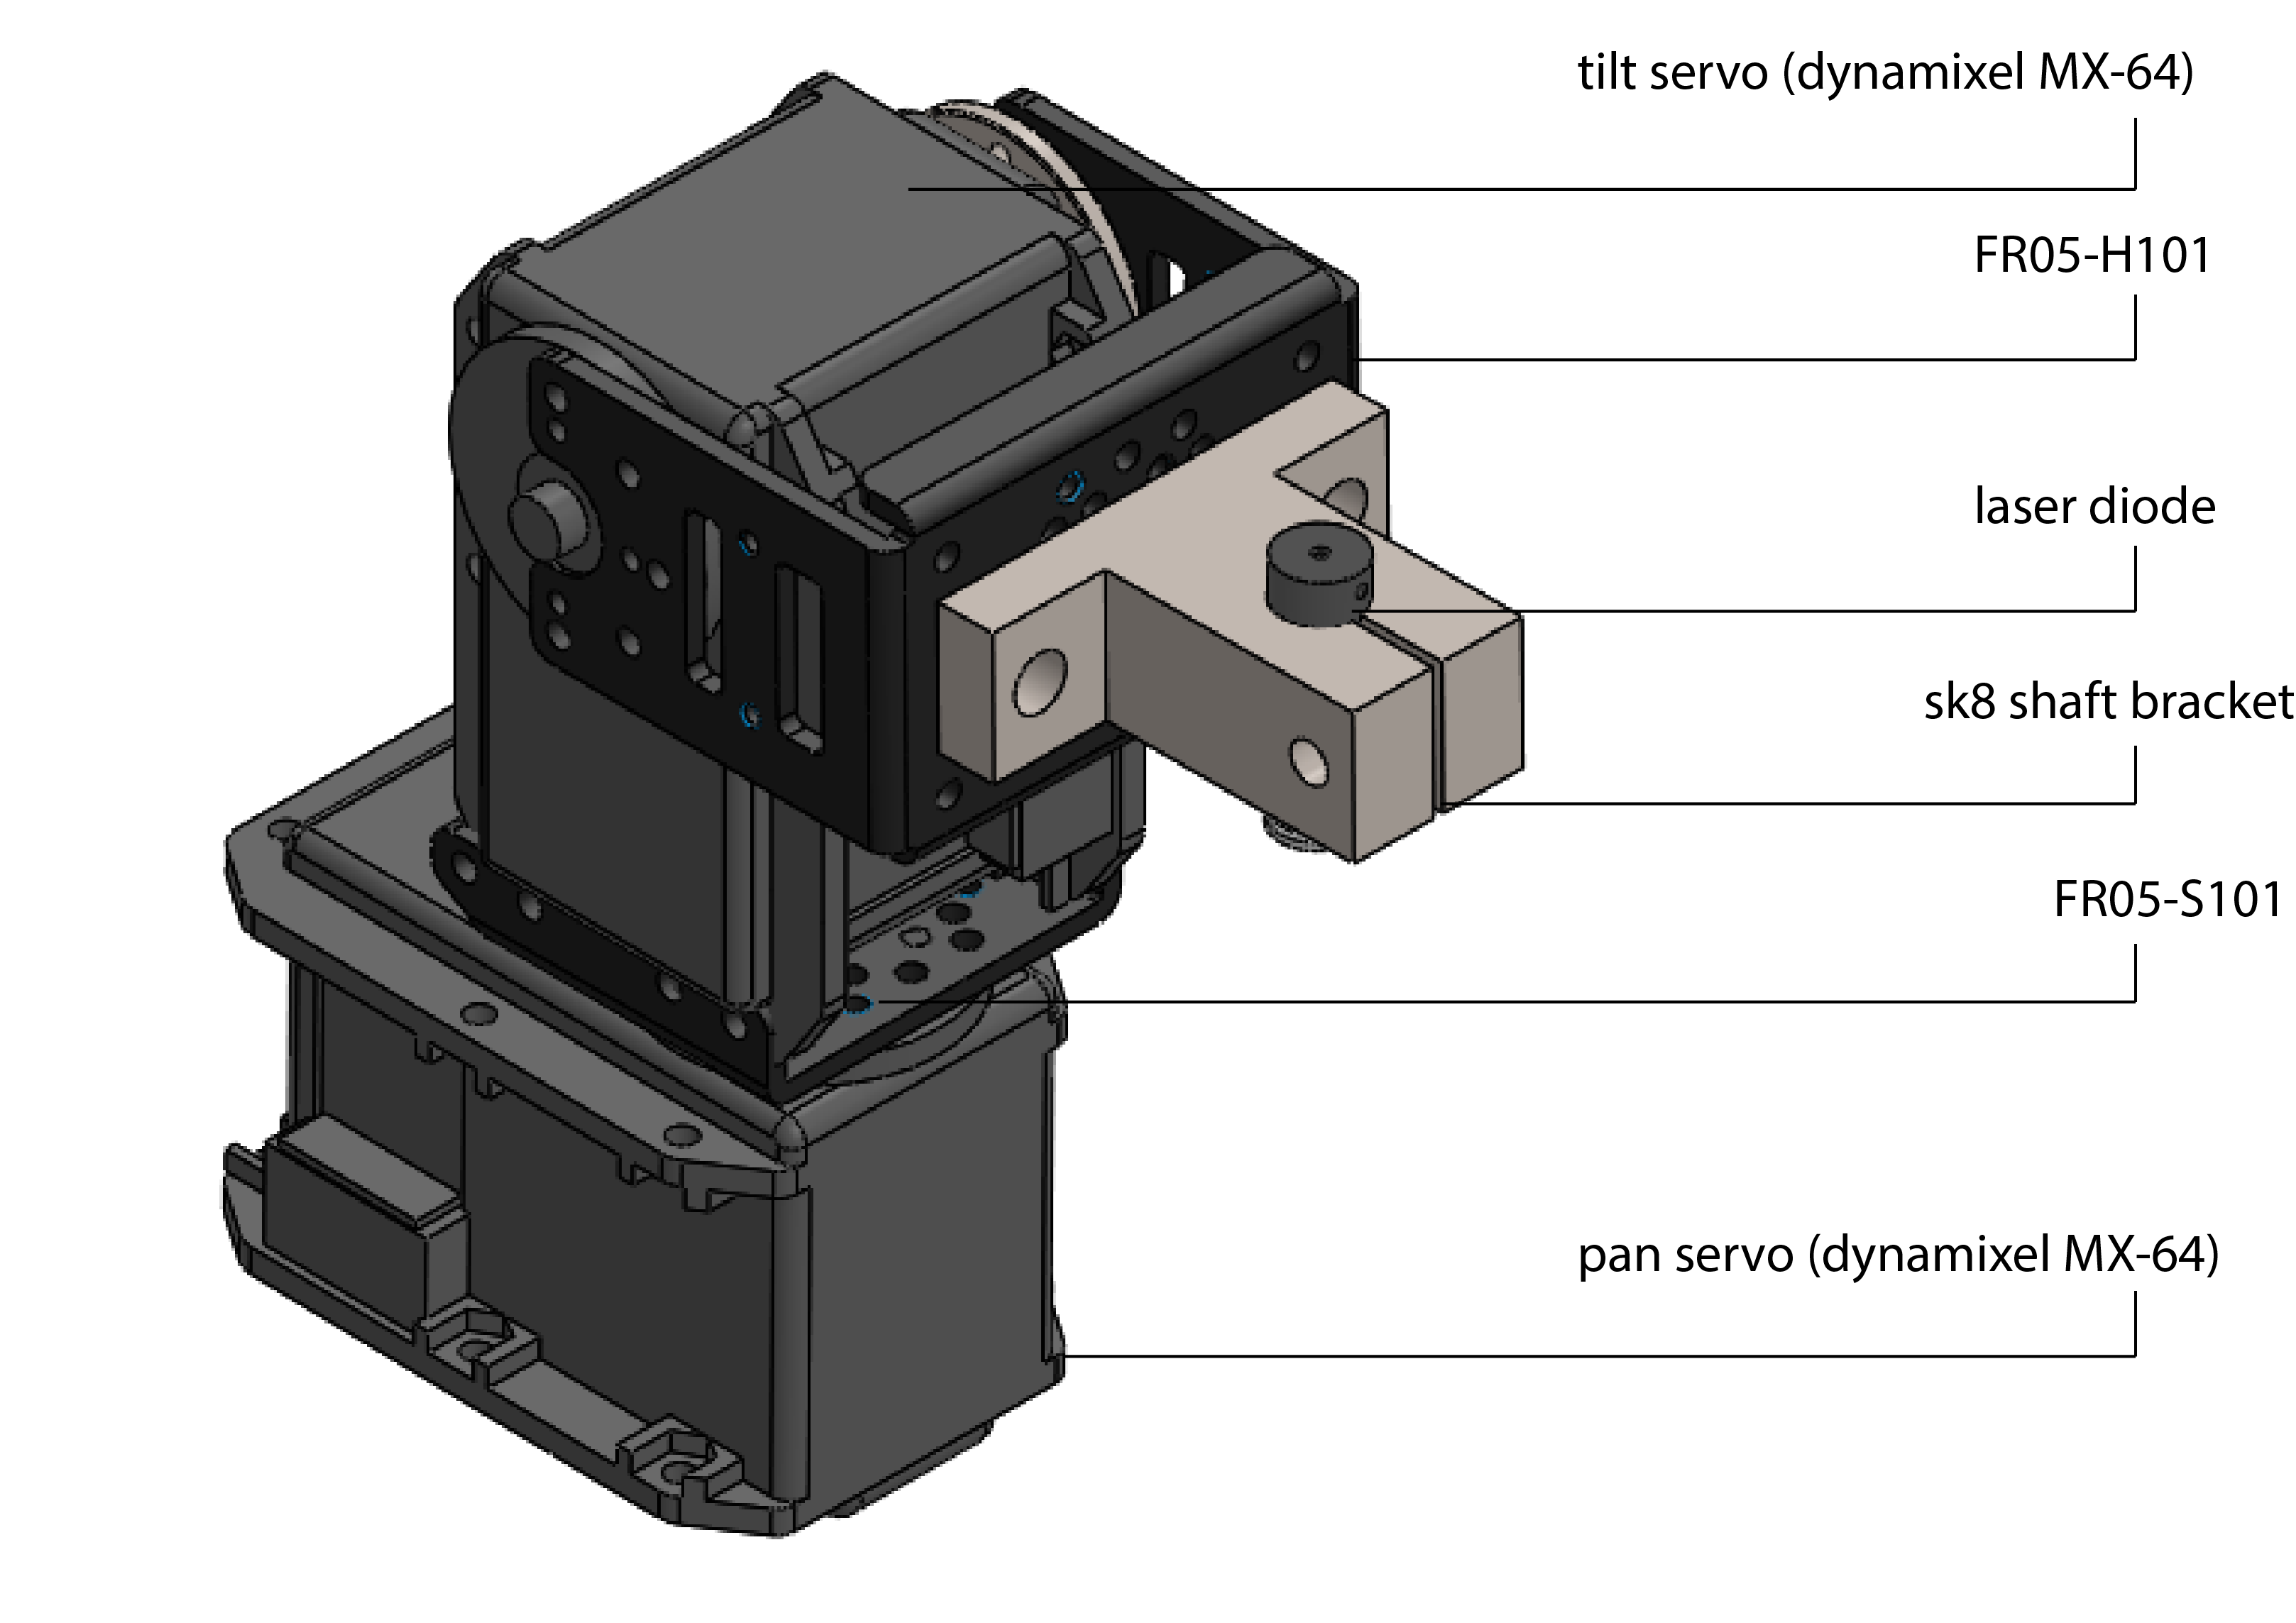
\includegraphics[width=\textwidth]{img/model23dCap.png}%
	\caption{Second Turret Model, 3D with Parts Names}
	\label{fig:model23DCap}
\end{figure}
As already mentioned, we are going to present a second and more powerful turret. Looking at figure \ref{fig:model2Photo}, \ref{fig:model23D} and \ref{fig:model23DCap} we can immediately see that there are some structural differences from the previous model, but those are already discussed in \ref{subs:secondModel}. Here, we want to discuss the new hardware, in particular motors and structural parts, which come from the ScorpionX MX-64 Robot Turret Kit by Interbotix \cite{MX64Turret}.
\subsection{Dynamixel MX-64T}
Quoting from \cite{web-MX64}:\\
\virgolette{\textit{The MX-64T Dynamixel Robot Servo Actuator is the newest generation of Robotis Dynamixel actuator; equipped with an onboard 32bit 72mhz Cortex M3, a contact-less magnetic encoder with 4x the resolution over the AX/RX series, and up to 3mpbs using the new TTL 2.0 bus. Each servo has the ability to track its speed, temperature, shaft position, voltage, and load. As if this weren't enough, the newly implemented PID control algorithm used to maintain shaft position can be adjusted individually for each servo, allowing you to control the speed and strength of the motor's response. All MX Series servos use 12v nominal voltage, so MX Dynamixels can be mixed without having to worry about separate power supplies. All of the sensor management and position control is handled by the servo's built-in microcontroller. This distributed approach leaves your main controller free to perform other functions.}}\\
So, we already know that those motors are more powerful than the ones used for the first model. Moreover, they are also compatible. The result is that we can reuse the same software interface written for the first turret without any issues, obtaining a more reliable model in term of accuracy, precision and trajectory smoothness. That confirms that things are done right also with the first turret, but we are facing its physical/hardware limitations. The results with the new turret are considerably better even without directly exploiting and tuning the more sophisticated functions offered by the new motors, such as built-in PID controllers or faster communication.
\subsection{Motor Specification}
\begin{figure}
	\centering
	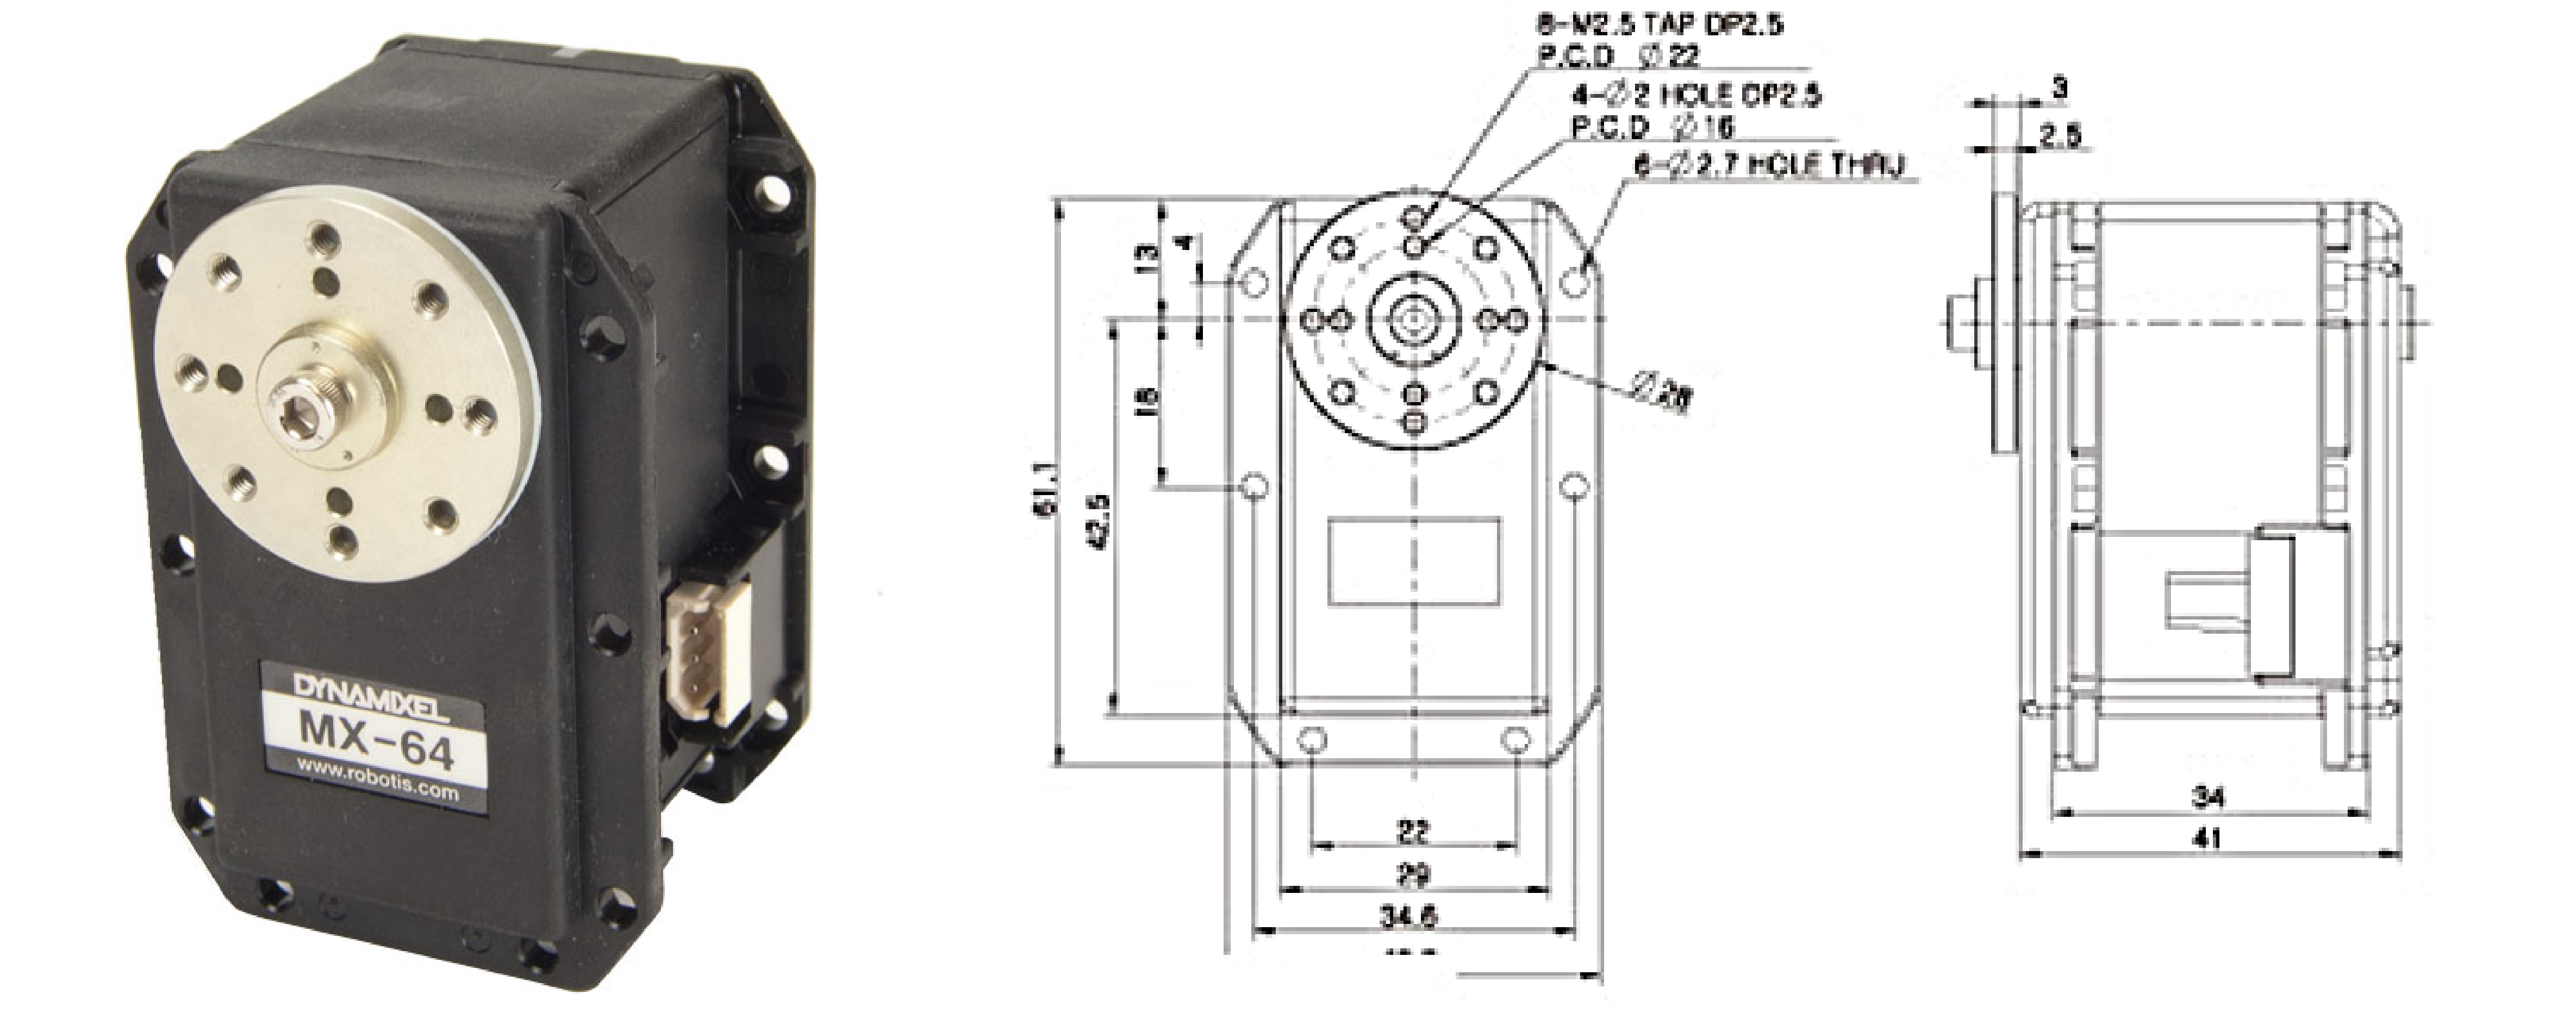
\includegraphics[width=\textwidth]{img/mx64.png}%
	\caption{Dynamixel MX-64}
	\label{fig:mx64}
\end{figure}
From the full datasheet \cite{datasheet-MX64} we report only two important specifications:
\begin{itemize}
    \item \textbf{Resolution}: $0.088^{\circ}$;
    \item \textbf{Communication Speed}: 8000 bps $\sim$ 4.5 Mbps.
\end{itemize}
As we can see, the resolution of those servos is roughly 3 times better than the Dynamixel AX-12. This is enough to make the new turret perform perfectly for our needs using exactly the same approach we use to solve the issues explained in \ref{subs:firstModel:issues}
\subsection{Other Components}
Though we use a 3V green laser diode on that turret, the other components are the same: \emph{Bioloid Bus Interface} for communication and \emph{Arduino Uno Board} for powering the laser (that time from the 3.3V output).\\
The structural parts are provided together with the ScorpionX MX-64 Robot Turret Kit. Figure \ref{fig:mx64Pieces} shows the components used from that kit: the turret base and the metal frames. Since the bracket of the tilt servo is too short, we had to mount the laser diode perpendicularly, obtaining the different structure already discussed.
\begin{figure}
	\centering
	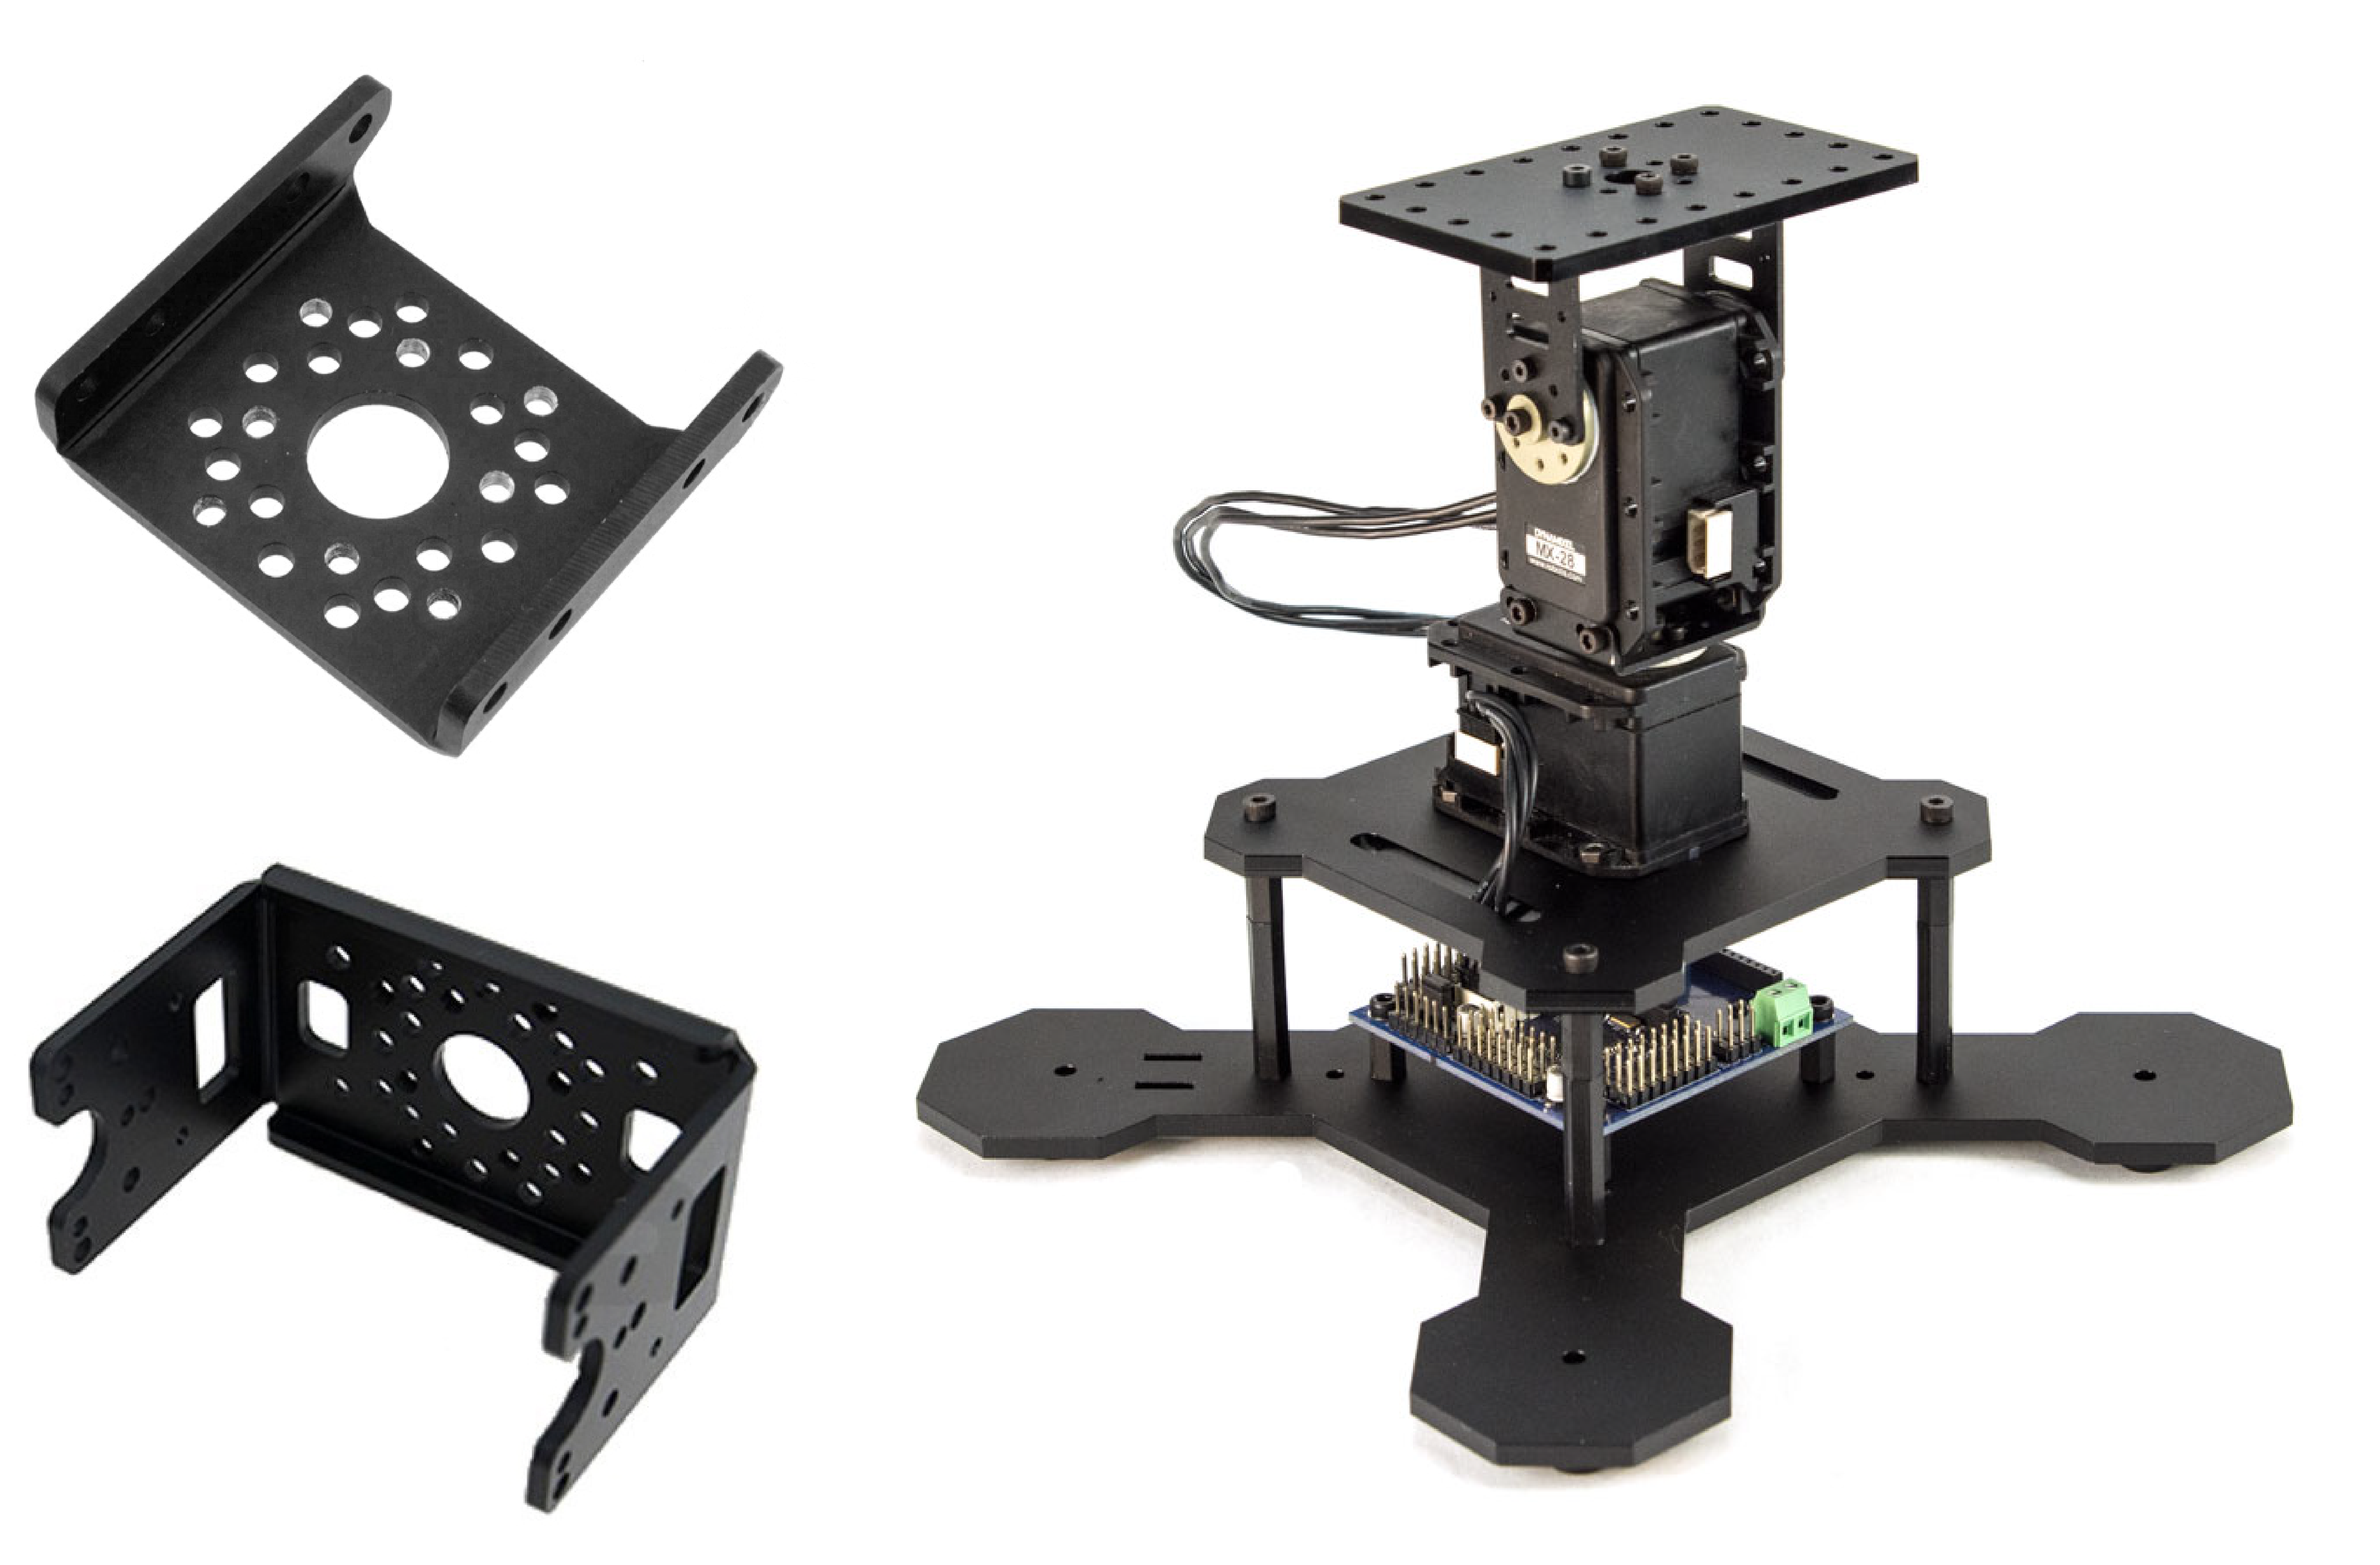
\includegraphics[width=.7\textwidth]{img/mx64Pieces.png}%
	\caption{\emph{Top-Left}: FR05-S101 Side Frame. \emph{Bottom-Left}: FR05-H101 Hinge Frame. \emph{Right}: ScorpionX MX-64 Robot Turret Kit.}
	\label{fig:mx64Pieces}
\end{figure}
\section{Arm IMU}
As explained in \ref{sec:1.2}, we need an arm IMU device to reconstruct the direction of human pointing. First, we present the Myo Armband, \virgolette{\textit{a gesture recognition device worn on the forearm and manufactured by Thalmic Labs. The Myo enables the user to control technology wirelessly using various hand motions. It uses a set of electromyographic (EMG) sensors that sense electrical activity in the forearm muscles, combined with a gyroscope, accelerometer and magnetometer to recognize gestures.}}. Obviously, we are interested only into the functions provided by gyroscope, accelerometer and magnetometer. We used such an expensive and mostly unnecessary device because it was what we already had.\\ However, our later work is based on a cheaper and more suitable device, the MetaMotionR board by Mbientlab, which can be mounted on a wrist band and provides a 9-axis IMU with Sensor Fusion. This is more convenient for our purposes, as it is easier to setup (it has a bluetooth driver for linux), more comfortable to wear (it is just like a watch) and also provides a LED for colour feedback and a small button (both are useful for our experiments and demos).
\begin{figure}
	\centering
	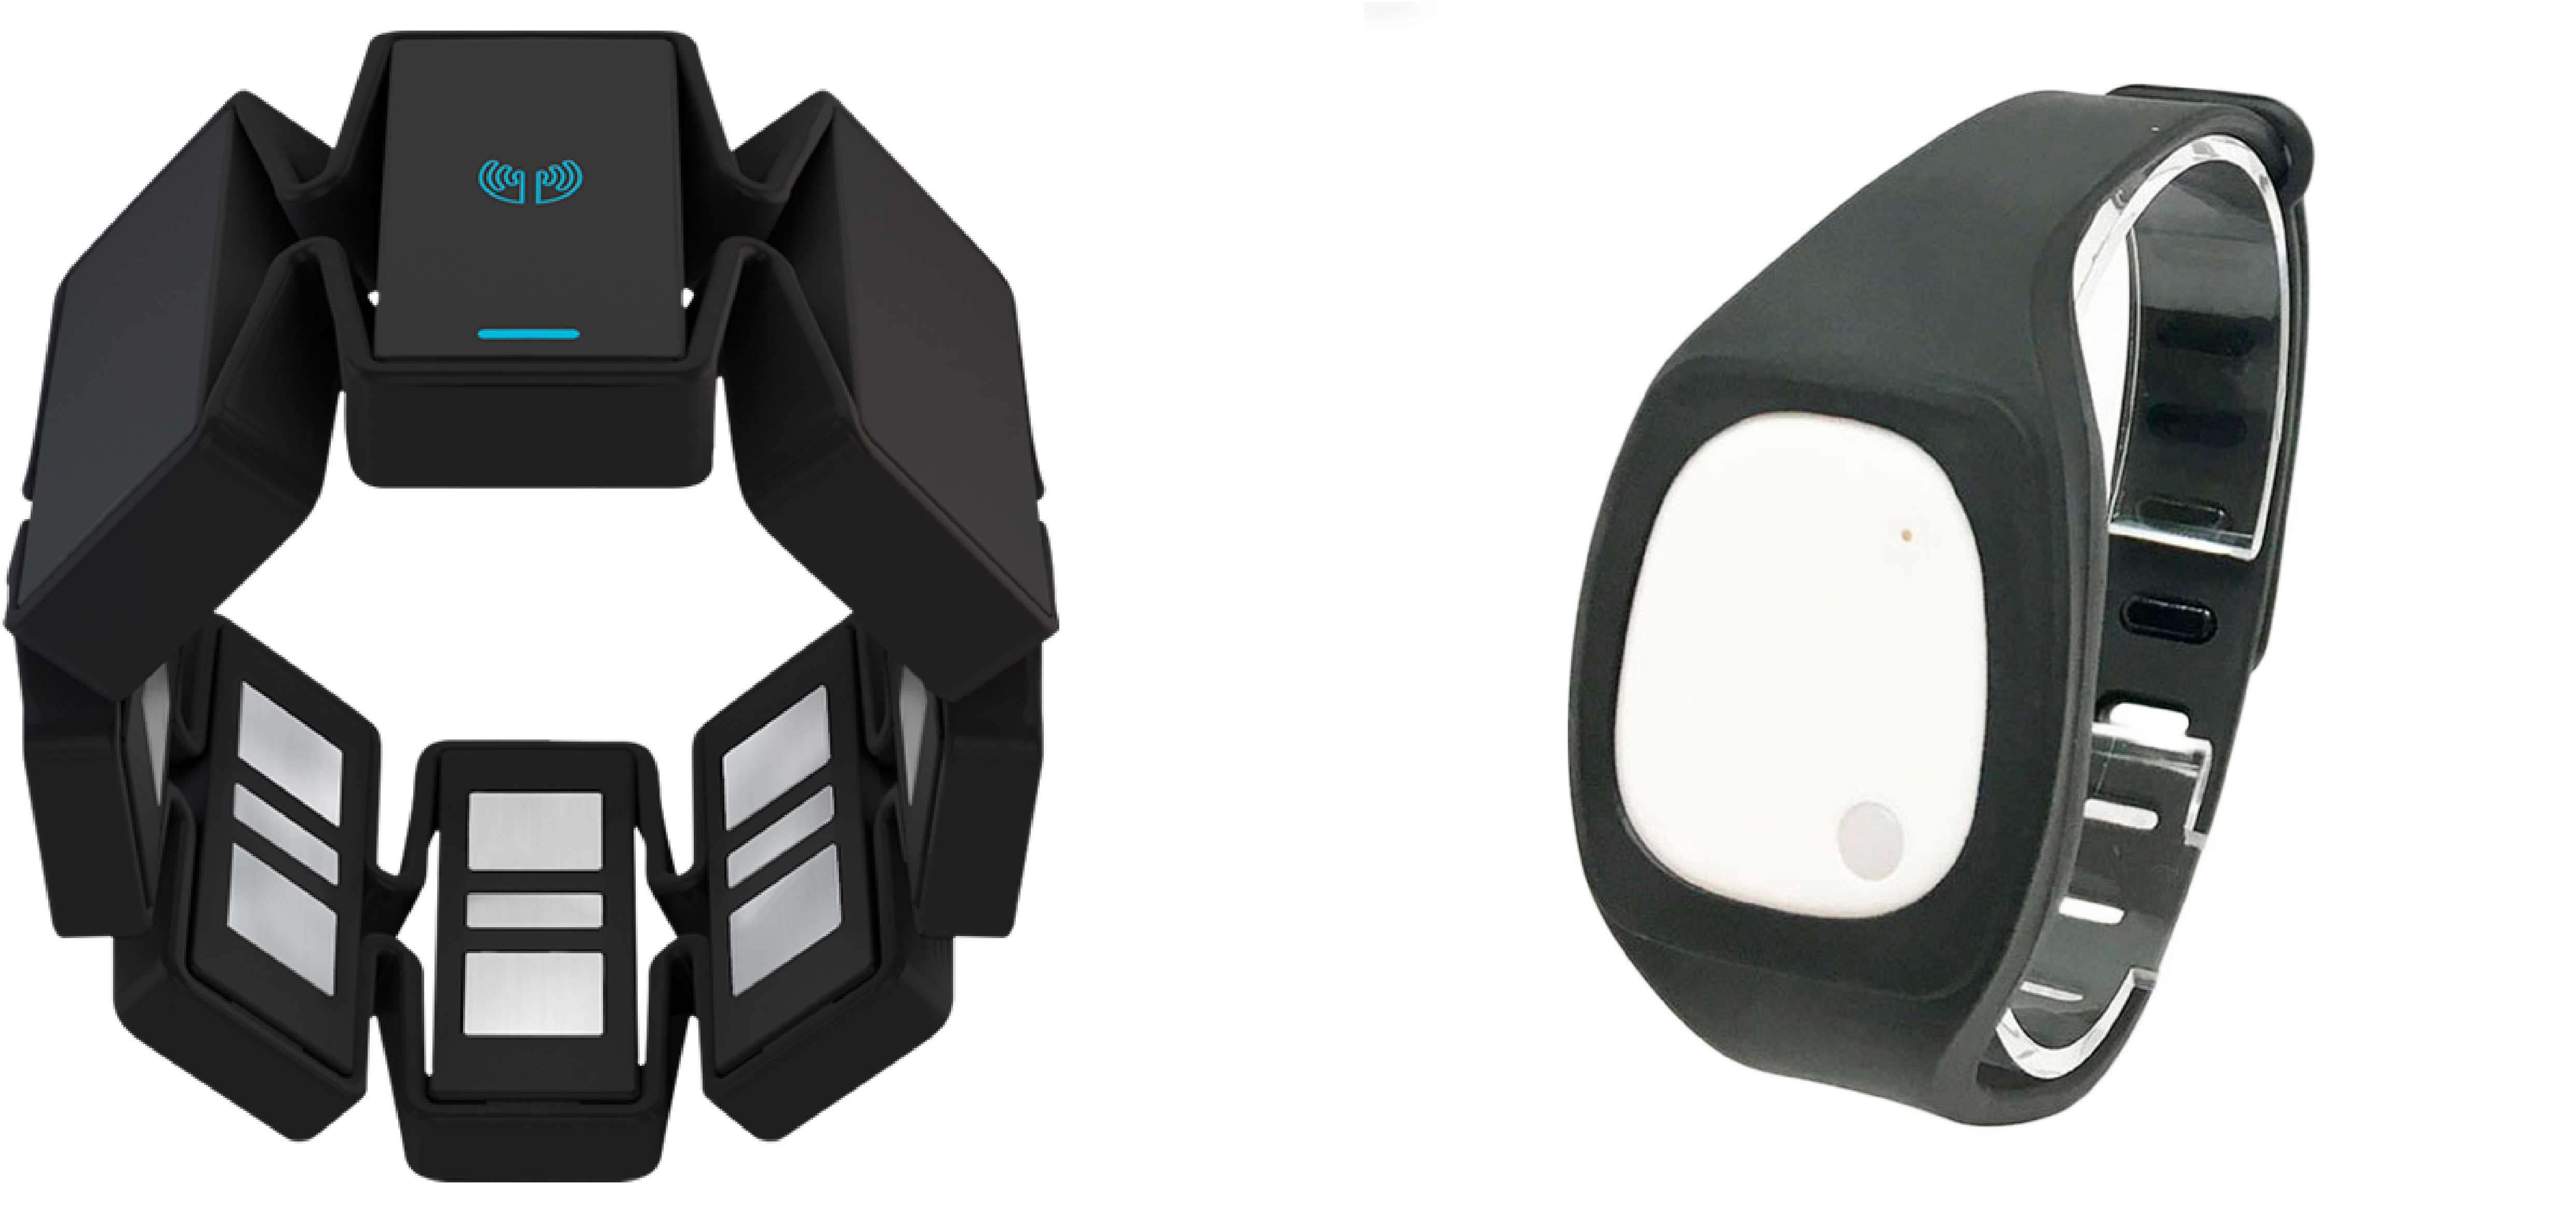
\includegraphics[width=\textwidth]{img/IMUS.png}%
	\caption{\tetbf{IMU Devices:} \emph{Left}: Myo Armband. \emph{Right:} MetaMotionR Wrist Band.}
	\label{fig:IMUS}
\end{figure}
\section{Kobuki}
\virgolette{\textit{iClebo Kobuki is a low-cost mobile research base designed for education and research on state of art robotics. With continuous operation in mind, Kobuki provides power supplies for an external computer as well as additional sensors and actuators. Its highly accurate odometry, amended by our factory calibrated gyroscope, enables precise navigation.}} \cite{kobuki}.\\
As already stated, one of the main application of our system is ground robot navigation. We developed a couple of demo using the \emph{Kobuki}, a groud robot suitable for our purposes. Note that we actually use a \emph{TurtleBot2}, but only its structure (i.e. \emph{Kobuki} base plus mounting platform). For example, we do not exploit the \emph{kinect} camera provided with the \emph{Turtlebot2}. Its structure is perfectly suitable to mount our turret on top of it (figure \ref{fig:kobukiTurret} and thus demonstrate our system.
\begin{figure}
	\centering
	\includegraphics[width=0.5\textwidth]{img/.jpg}%
	\caption{Turtlebot2 (with Kobuki base)}
	\label{fig:turtlebot}
\end{figure}
\chapter{Software Implementation}\label{chap:3}
Now that we have all the theoretical and practical elements of the system, here we report all the work done to implement it on a software side. That includes code written from scratch and also code used to interface with already existing parts. This chapter can be divided in 4 parts:
\begin{enumerate}
    \item introduction of all the basics libraries used;
    \item description of the code implemented to control the turret and the solution adopted to overcome the issues mentioned in \ref{subs:firstModel:issues};
    \item explanation on how we interface with the arm pointing system and the relative localization procedure;
    \item demos implementation.
\end{enumerate}
Experiment setups and procedures are left for chapter \ref{chap:4}.

\section{Libraries and Frameworks}
The system developed is composed by many modules handling different functionalities. It is worth to mention a couples of libraries and frameworks which are widely used throughout the project, as some of them are also primary to understand the implementation. In the next section we will give an overview of:
\begin{itemize}
	\item \ac{ROS} Kinetic Kame
	\subitem \texttt{rospy} 1.12.13
	\subitem \texttt{rosbag} 1.12.13
	\subitem \texttt{tf} 1.11.9
	\item \texttt{Dynamixel Workbench} and \texttt{Dynamixel SDK}
	\item \texttt{NumPy} 1.14.3
	\item \textttt{Matplotlib} 2.2.2
	\item \texttt{pandas} 0.23.0
\end{itemize}
The programming language used for development is Python 2.7.12.\\

\subsection{\acf{ROS}}
\ac{ROS} is a open-source\footnote{Main client libraries and tools are under the terms of the BSD license (\url{https://en.wikipedia.org/wiki/BSD_licenses}).} meta-operating system for robots \cite{ros}. \ac{ROS} is the industry and research standard framework for robotics and it is aimed to help software developers to  create robotic applications.\\

Its primary goal is to support code reuse in robotics research and development. \ac{ROS} is a distributed framework of processes (aka Nodes) that enables executables to be individually designed and loosely coupled at runtime. These processes can be grouped into Packages and Stacks, which can be easily shared and distributed. \ac{ROS} also supports a federated system of code Repositories that enable collaboration to be distributed as well. This design, from the filesystem level to the community level, enables independent decisions about development and implementation, but all can be brought together with \ac{ROS} infrastructure tools.\\
At the lowest level, ROS offers a message passing interface that provides inter-process communication and is commonly referred to as a middleware.
The ROS middleware provides these facilities \cite{ros:core-components}:
\begin{itemize}
    \item publish/subscribe anonymous message passing
    \item recording and playback of messages
    \item request/response remote procedure calls
    \item distributed parameter system
\end{itemize}
In addition to the core middleware components, ROS provides common robot-specific libraries and tools to get a robot up and running quickly. Here are just a few of the robot-specific capabilities that ROS provides:
\begin{itemize}
    \item Standard Message Definitions for Robots
    \item Robot Geometry Library
    \item Robot Description Language
    \item Pose Estimation
    \item Localization
    \item Mapping
    \item Navigation
\end{itemize}
in particular, the \emph{Robot Geometry Library} is widely used for that project.
\subsubsection*{Robot Geometry Library: tf}
A common challenge in many robotics projects is keeping track of where different parts of the robot are with respect to each other. For example, if one wants to combine data from a camera with data from a laser, he needs to know where each sensor is, in some common frame of reference. This issue is especially important for humanoid robots with many moving parts. This problem is addressed in ROS with the \texttt{tf} (transform) library, which will keep track of where everything is in the robot system.

Designed with efficiency in mind, the \texttt{tf} library has been used to manage coordinate transform data for robots with more than one hundred degrees of freedom and update rates of hundreds of Hertz. The \texttt{tf} library allows one to define both static transforms, such as a camera that is fixed to a mobile base, and dynamic transforms, such as a joint in a robot arm. One can transform sensor data between any pair of coordinate frames in the system. The \texttt{tf} library handles the fact that the producers and consumers of this information may be distributed across the network, and the fact that the information is updated at varying rates.\\
\texttt{tf} lets the user keep track of multiple coordinate frames over time. \texttt{tf} maintains the relationship between coordinate frames in a tree structure buffered in time, and lets the user transform points, vectors, etc between any two coordinate frames at any desired point in time.

\subsubsection*{Nodes}
\ac{ROS} nodes are executable files that use \ac{ROS} to communicate with other nodes. Nodes are usually fine grained processes that perform precise computations. To communicate, nodes use a ROS client library to publish or subscribe to \emph{topics} or \emph{services}. Different Nodes can run on different hardware while being in the same \ac{ROS} system.

\subsubsection*{Bags}
Another function of \ac{ROS}, are \lstinline|rosbag| files. Bags are a format for saving and playing back ROS message data. Bags are an important mechanism for storing data, such as sensor data, that can be difficult to collect but is necessary for developing and testing algorithms.


\subsection{Dynamixel SKD}
The \texttt{ROBOTIS Dynamixel SDK} is a software development kit that provides Dynamixel control functions using packet communication. The API of Dynamixel SDK is designed for Dynamixel actuators and Dynamixel-based platforms. It is based on C/C++ programming. The Dynamixel SDK supports all Dynamixel series developed by \texttt{ROBOTIS}. For example, all series such as AX, RX, EX, MX, XL, XM, XH, PRO-L, PRO-M and PRO-H are supported by packet communication.
\begin{figure}
	\centering
	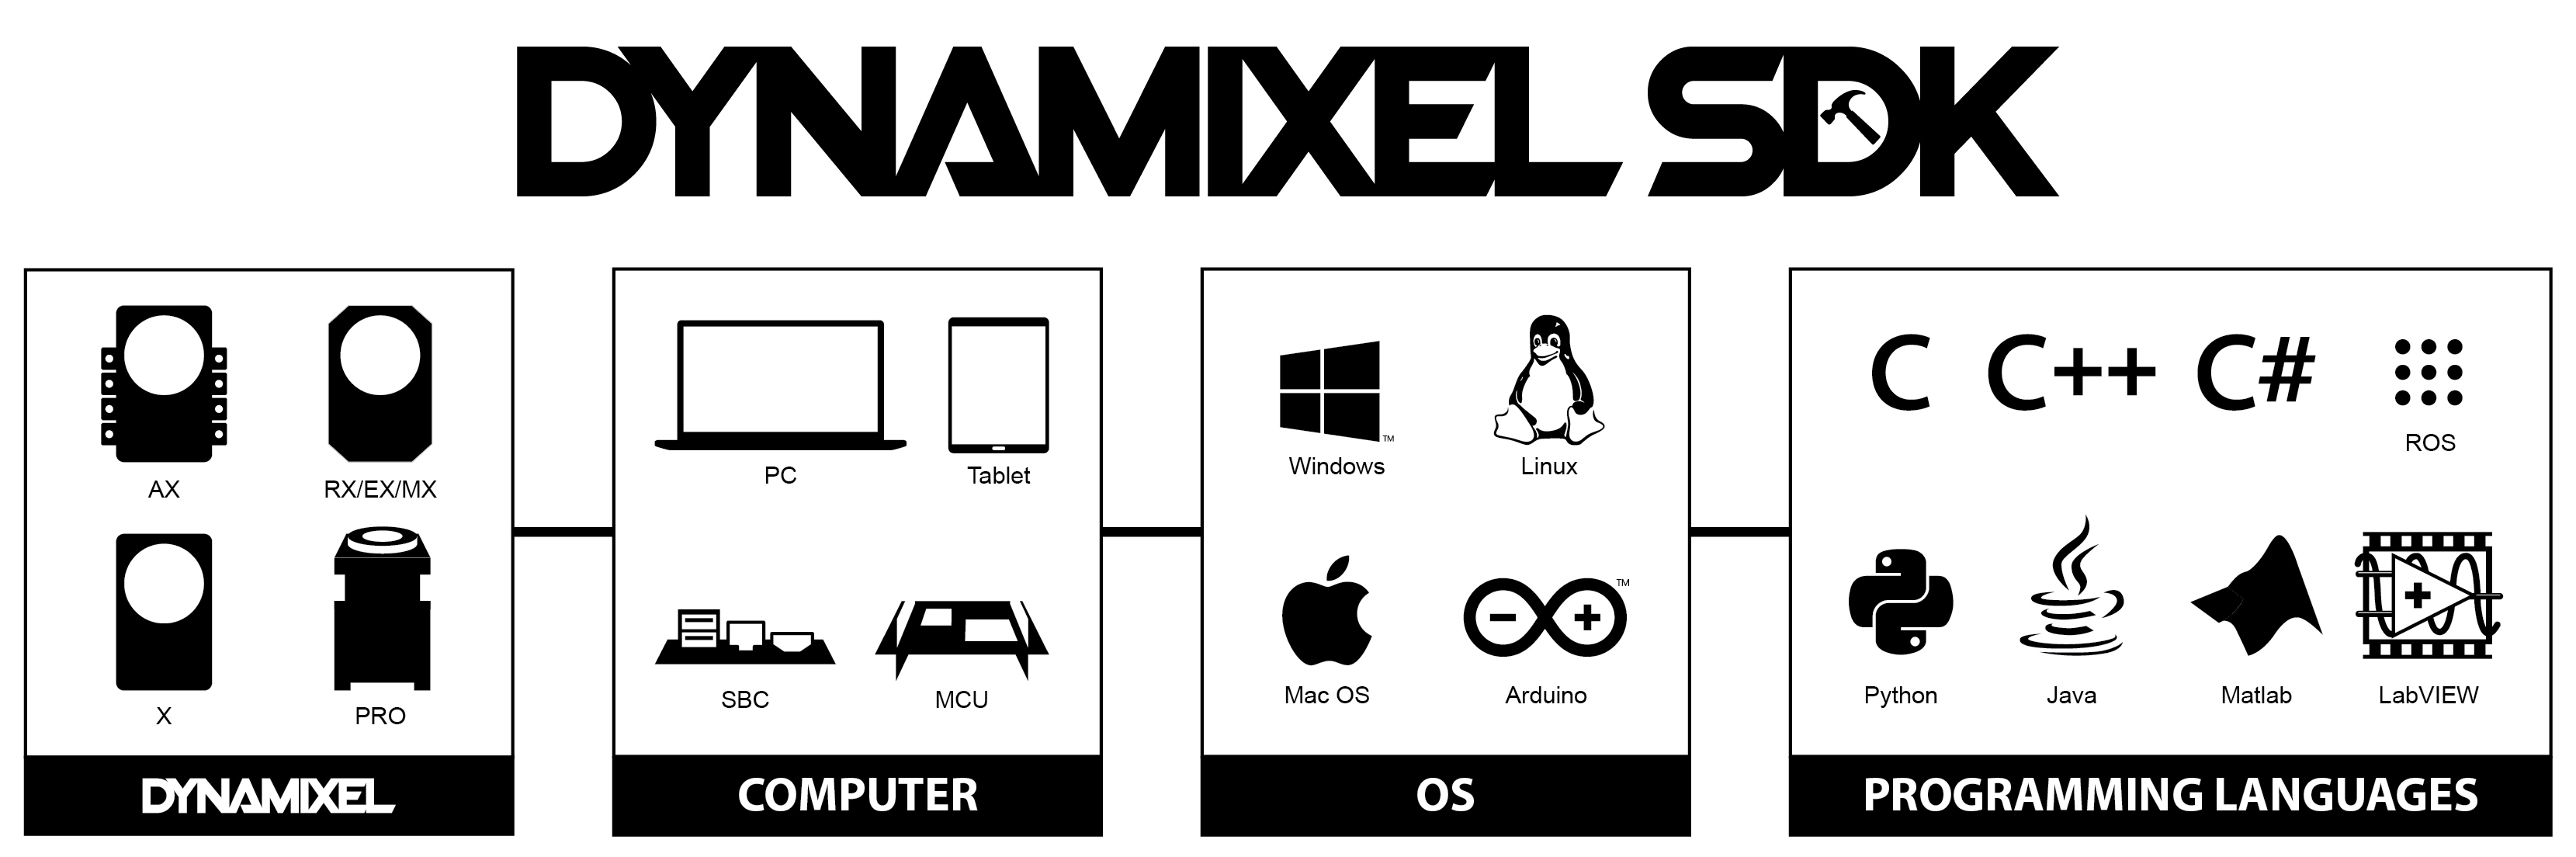
\includegraphics[width=\textwidth]{img/sdk.jpg}%
	\caption{Dynamixel SDK}
	\label{fig:turretPipeline}
\end{figure}

\subsection{Dynamixel Workbench}
Dynamixel-Workbench is dynamixel solution for ROS. This metapackage allows one to easily change the ID, baudrate and operating mode of the Dynamixel. Furthermore, it supports various controllers based on operating mode and Dynamixel SDK. These controllers are commanded by operators.


\subsection{Numpy}
NumPy is the fundamental package for scientific computing with Python \cite{numpy}. It contains among other things:
\begin{itemize}
    \item a powerful N-dimensional array object
    \item sophisticated (broadcasting) functions
    \item tools for integrating C/C++ and Fortran code
    \item useful linear algebra, Fourier transform, and random number capabilities
\end{itemize}

Besides its obvious scientific uses, NumPy can also be used as an efficient multi-dimensional container of generic data. Arbitrary data-types can be defined. This allows NumPy to seamlessly and speedily integrate with a wide variety of databases.
\subsection{Matplotlib}
Matplotlib is a Python 2D plotting library which produces publication quality figures in a variety of hardcopy formats and interactive environments across platforms \cite{matplotlib}. Matplotlib can be used in Python scripts, the Python and IPython shells, the Jupyter notebook, web application servers, and four graphical user interface toolkits.\\

Matplotlib makes plotting high quality graphs accessible to anyone. With Matplotlib it is possible to generate a wide variety of types of plots from histograms to scatter plots with just a few lines of code.\\

Matplotlib tries to make easy things easy and hard things possible. One can generate plots, histograms, power spectra, bar charts, errorcharts, scatterplots, etc., with just a few lines of code. 
Matplotlib uses a MATLAB-like interface. Power user have full control of line styles, font properties, axes properties, etc, via an object oriented interface or via a set of functions similar to MATLAB one.
\subsection{pandas}
\label{sec:pandas}
pandas\footnote{The name is written in lowercase letters.} is an open source community supported, BSD-licensed library providing high-performance, easy-to-use data structures and data analysis tools for Python. pandas is still in active development and since it has seen a growth in adoption, on the official documentation multiple guides are present to help shifting from another environment or language like R.

\section{Turret Software Implementation}
First, we must recall what are our goals. We want to be able to drive a laser dot on a given surface (i.e. the floor) by setting its \emph{x} and \emph{y} coordinates (the \emph{z} would be implicit on the floor). This must be done with a good precision and also with high frequency, as we want to draw nice and smooth trajectories with the laser. To do so, we can only control two Dynamixel servos, setting their angles values accordingly to the inverse kinematics solved in \ref{sec:1.1}.\\
So, we will describe how we implement the turret model and then the interface written to control the motors and achieve our goals.
\subsection{Turret Model Implementation}
The two turret models are implemented as ROS node containing the inverse kinematic equation and the code to publish the \texttt{tf tree} of the turret. Those models, in fact, are simply implemented as a chain of \texttt{tf frames}. In that way, we can easily keep track of the position/transformation of our frame, corresponding to our \emph{pan} and \emph{tilt} angle. This is an immediate implementation of the logic already depicted in figures \ref{fig:firstModelRefFrame} and \ref{fig:secondModelRefFrame}.\\
So, those are the nodes in charge to compute and keep track of the values of our two DoF.


\subsection{Motors Controller}
The drivers for both the AX-12+ and the MX-64 Dynamixels are provided by the \texttt{dynamixel sdk}. Moreover, the \texttt{dynamixel workbench} offers ROS interfaces to work with the official sdk. That is one of the most crucial part of software, because it is directly related to the issues mentioned in section \ref{subs:firstModel:issues}. As a matter of fact, it is where we intervene to solve those issues, which are mostly due to the slow communication protocol. As a matter of fact, we motors are not able to process all the points composing the trajectory that we need to send at 50Hz and they simply drop them. That happens because each time a command is sent through the bus interface, each motors has to reply with an acknowledgment. So, we disable all kind of response from the servos, assuming that once a command is sent, it will be properly executed. Moreover, we hack the drivers to be sure that the PC will not wait for motors replies. That is a bit tricky as, even though the low level function to write the servos registries without wait for reply exists, we have to find and expose it through the workbench libraries.\\
Given that, we are able to draw our smooth trajectories in the simplest way possible: sending points at a fixed rate with the servos in joint mode. \emph{Joint mode} means \emph{position control}. In other word, we can directly specify the value of the position/angle we want the servo to reach to the servo itself. Its internal controller will move the motor accordingly.\\
That works fine with the first turret model, but also with the second one. Even better, the \emph{MX-64} based turret works perfectly thanks to its better servo resolution.\\

Even if the two turret model could use the same interface, the software project contains two different ones as, for the first turret, we use an unofficial low level driver that is tightly coupled with the architecture of the Dynamixel \emph{AX-12+} itself and thus is not reusable. On the contrary, for the second turret, the code is rewritten to directly exploit the generic ROS service interface offered by the \texttt{dynamixel workbench}. That code would also work with the first model.\\
Finally, we have a useful module to publish the points composing the desired trajectory.

\subsection{Laser Turret Complete Picture}
Now that all the software parts composing the turret have been introduced, we can put everything together to understand exactly how the code is modulated and which module is in charge of what. Here we will consider the file related to the \emph{MX-64} turret. Figure \ref{fig:turretPipeline} give us an idea.
\paragraph{tf\_broadcaster} is the module containing and simulating the geometrical model of the turret. It also computes the inverse kinematic of the laser dot. So, this is the piece of software in charge of computing the joints position (i.e. \emph{pan} and \emph{tilt} values) corresponding to the laser dot goal position (expressed in the reference frame of the turret). It only takes a 3D point as input, but serves all our purposes: it can be used to draw a trajectory, as long as ones send a stream of point as input; it can be used to follow the human pointing, after the relative localization is done; it can, of course, mark a single spot on the floor (as we need it for the experiments).
It will publish those values and update its internal representation of the turret accordingly, but it will not directly send the commands to move the motors. This is very convenient, as it allows us to simulate the system even without a physical turret and decouples the logical model from the physical controller.\\
\paragraph{turret} module contains that physical controller. Again, that code is written with the idea of making the system modular. In fact, this class leverages on the \texttt{dynamixel workbench} to send commands to any Dynamixel motors. In that way, as long as we are working with a device which needs to set only two angles (e.g. \emph{pan} and \emph{tilt} unit), we can plug into the system any turret built with any Dynamixel motor model. Needless to say, that was helpful when we had to deal with two different turret models.\\
\paragraph{trajectory\_publisher} is needed to decide the shape of the trajectory to draw. Then, it will publish each point at a fixed rate to the interface provided by \texttt{tf\_broadcaster}. In that way, the laser dot will follow the desired trajectory. We can draw many different shapes, but in our experiments and demos we use the \virgolette{$\infty$} shape.

\begin{figure}
	\centering
	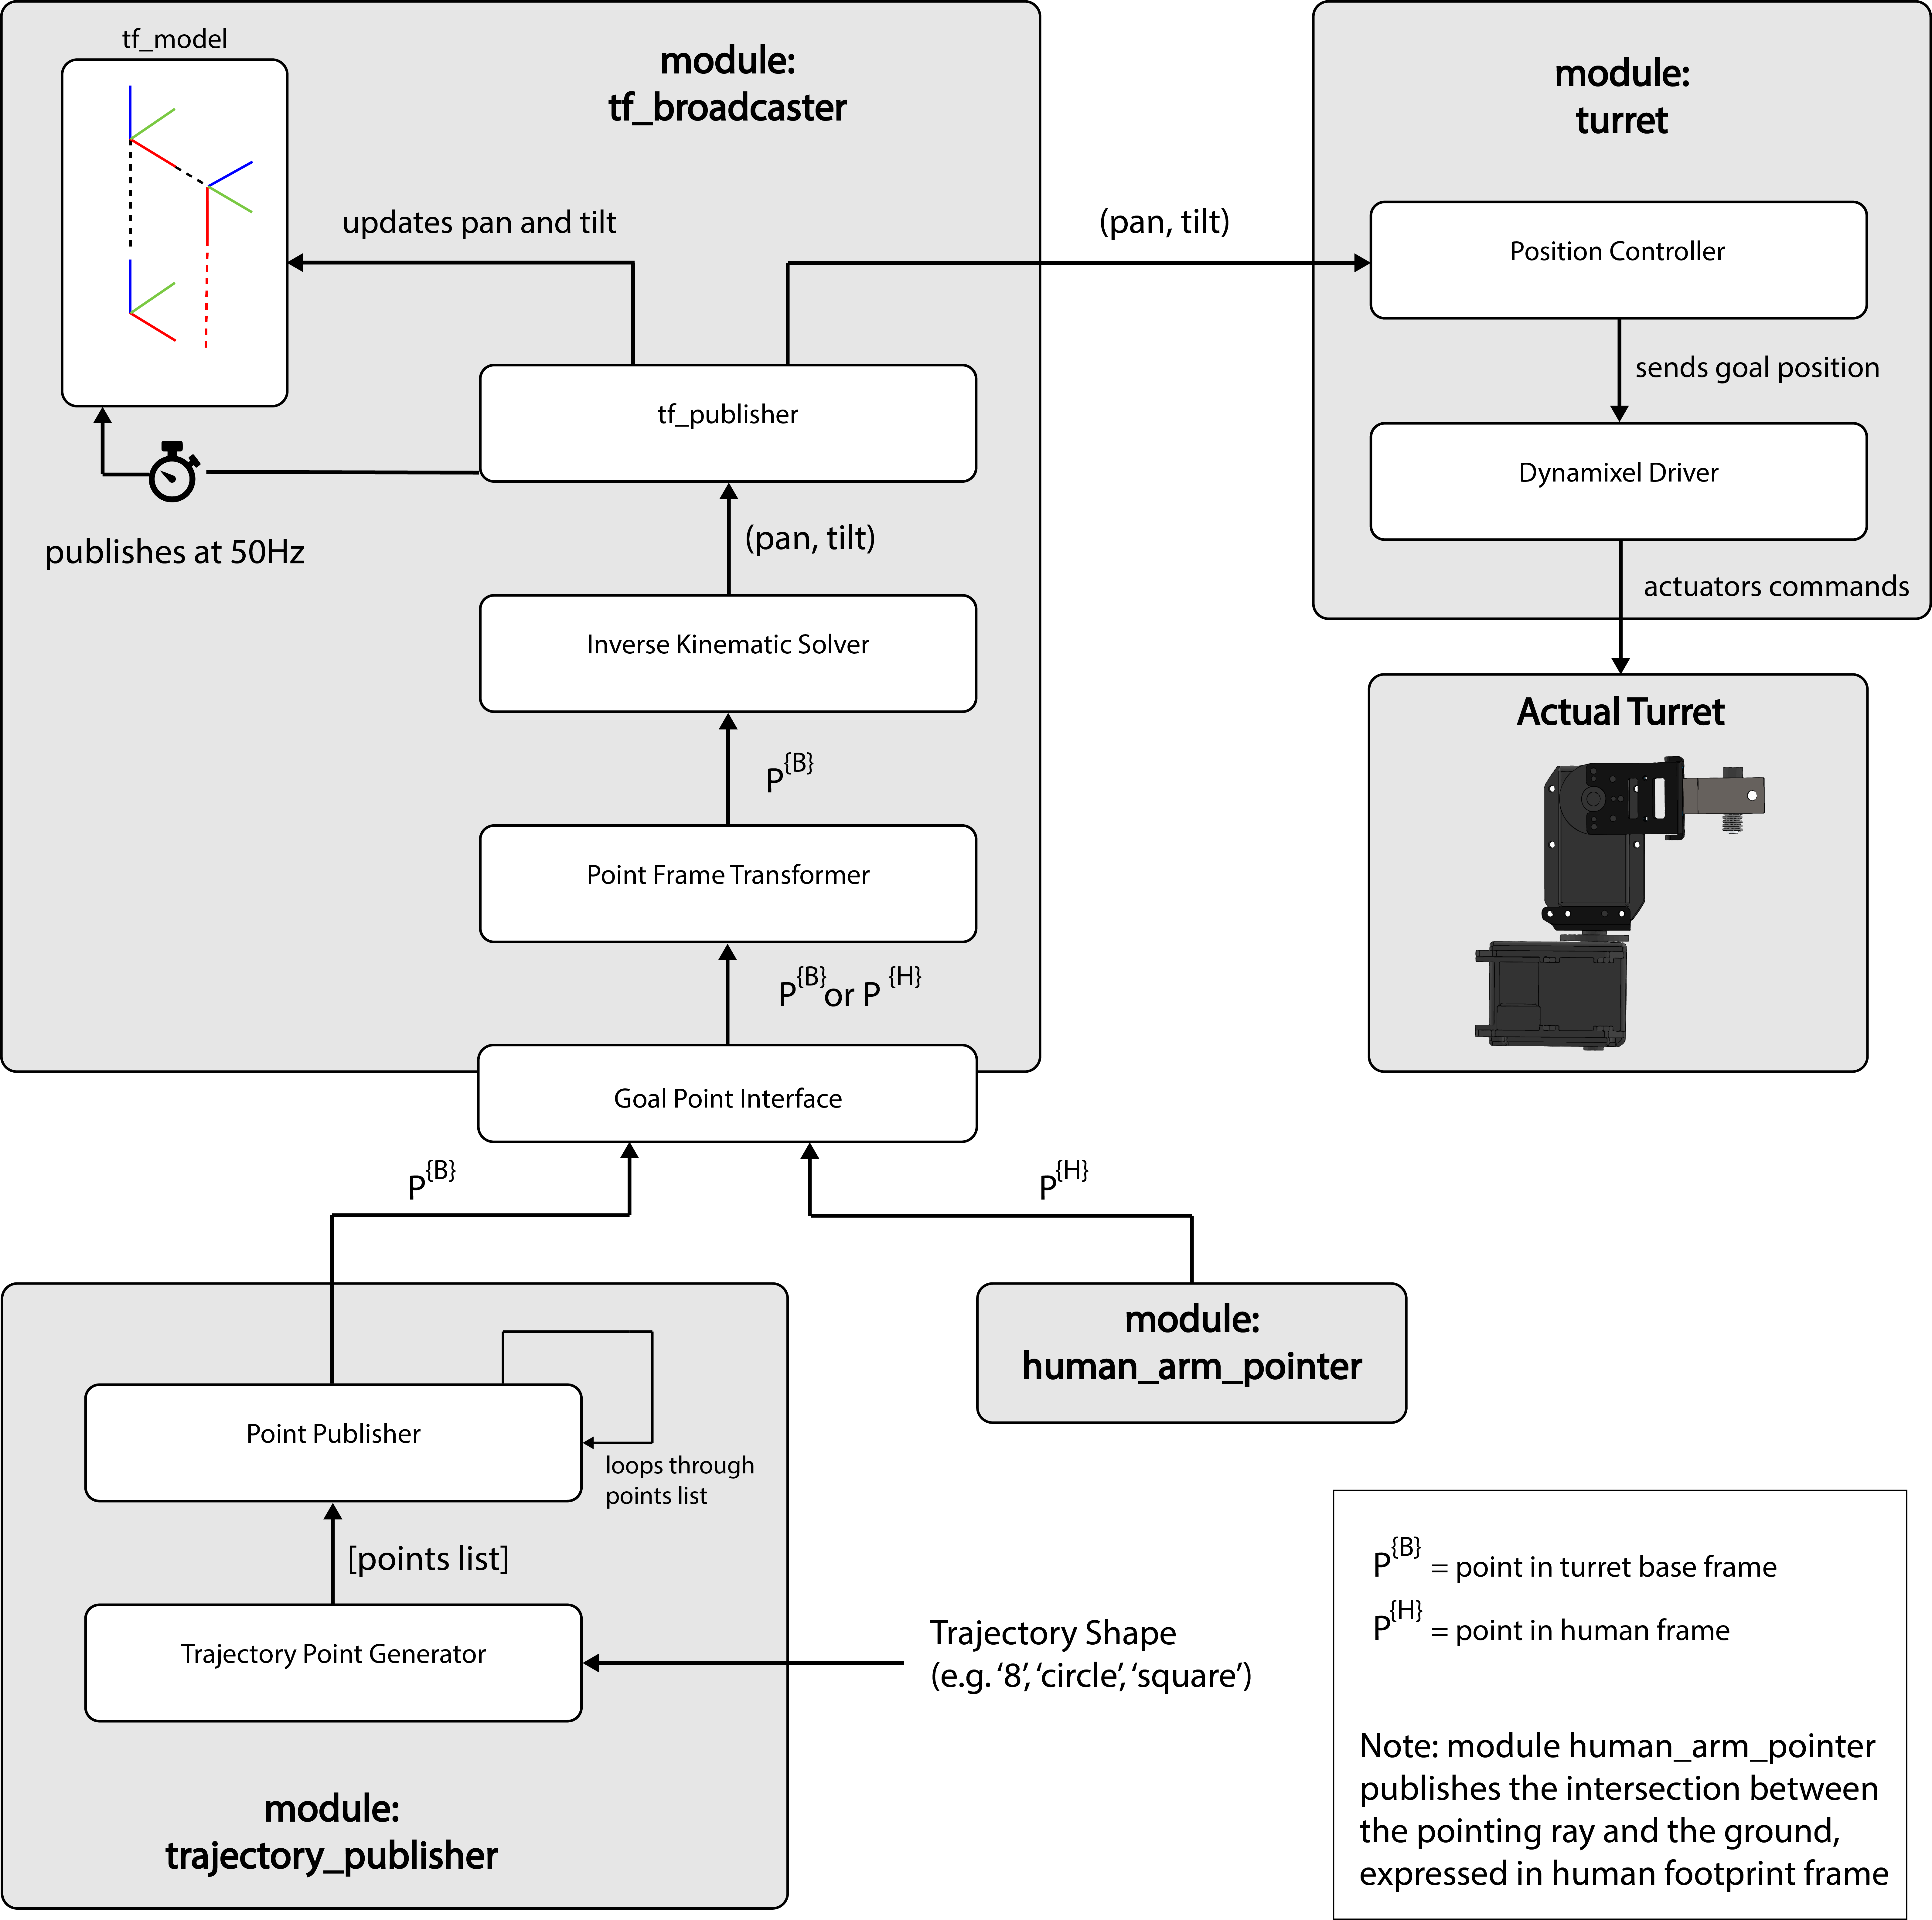
\includegraphics[width=\textwidth]{img/turretPipeline.png}%
	\caption{Laser Turret Implementation, the Complete Picture}
	\label{fig:turretPipeline}
\end{figure}


\section{Pointing Software Implementation}
As explained in section \ref{sec:1.2}, we are using the human pointing model suggested and implemented for \cite{gromov2018robot}. The geometry already presented in that section is very convenient as it can be implemented directly into code, as in the \textbf{arm\_node} module.\\
Thus, is very simple to understand how that part works: we receive as input the quaternions (i.e. the rotation) from the wearable IMU. In that way we can determine the direction of the pointing ray that we know has its origin between the eyes and passes through the fingertip of the human, exactly as previously shown in figure \ref{fig:pointingModel}. That requires also that certain measures of users' bodies are known. In particular, for each user we take the height which goes from the ground to the centroid of the head, from the shoulder to the wrist and from the wrist to the fingertip\\ 
We will not explain that code in details since it was not developed for that thesis, but we will mention one interesting fact related to pointing on the floor and the differences occurred when implementing the pointing on the wall (that part was developed for the thesis).
\subsection{Pointing on the Floor}
Keeping in mind that the pointing ray is an infinite line, we can easily see that there is a problem: when the human is pointing above the horizon (i.e. is not pointing on the floor), the ray will be still intersecting the plane behind the human. Luckily, for how things have been defined in \ref{eq:intersection}, we can simply check whether $s_I \geq 1$ to be sure that the intersection is ahead of the human. If not (also if the ray is parallel to the floor), we do not have a valid intersection, thus we return a pose for the human made with \texttt{NaN} values.
\subsection{Floor vs Wall}
As already stated, for that thesis we implemented also a demo with the user pointing on the wall. The implementation for the pointing itself was pretty straightforward, as it is similar to the one on the floor, but there are a couple of details that are implicit when pointing on the floor and that must be taken into account for the wall case. In fact, assuming that the human is standing on a flat plane perpendicular to him, which is a fair assumption for our system, we already know the distance from the floor (i.e. $0$) and its orientation. So, we know that if the human is not pointing above the horizon, we have an intersection. However, in the wall case, we have to explicitly know and set the distance of the human from the wall and its orientation to intersect the pointing ray. That makes the demo for our system on the wall limited by those initial conditions that, on the contrary, can be implicitly taken for granted in the floor case.


\section{Relative Localization Software Implementation}
As for the the pointing, the relative localization (relloc) implementation is the same proposed in \cite{gromov2018robot}. However, that code was written to work with a drone, so a flying robot with an odometry which is slightly different from a ground robot (and a laser point). For that thesis, only a couple of modifications were needed to interface the turret and then replace the drone with the laser dot. The result can be seen in \textbf{motion\_relloc} module. In that section we will give an overview of how that procedure is implemented in terms of input and output.
\subsection{Relloc Input}
As already explained in \ref{sec:relloc}, the relloc procedure takes as input a set of pairs composed by the position of the laser dot in the turret frame and the \emph{corresponding} pointing ray in human frame. \emph{Corresponding} means that we want to get the data of the ray generated by the human while the turret was marking that particular point with the laser. This is crucial, because it means that data must be synchronized precisely. This also explains why we wanted the turret to be  as precise, fast and smooth as possible. Thus, we are sending trajectory point to the turret at $50 Hz$ and collecting data from the arm IMU at the same rate.\\
To build our input set we specify the duration of the interaction in seconds (usually is $5s$ in our demos) and the number of pairs to sample (usually $250$). Since in $5$ seconds at $50 Hz$ we collect exactly $250$ pairs, it means that we usually sample the whole set. We use those values as $5$ second are enough to draw an $\infty$ shaped trajectory with a speed that allows the human to follow the laser easily.
\subsection{Relloc Output}
Recalling what was written in section \ref{sec:relloc}, the output of the relloc is the transformation:
\begin{align}
	\rho = [t_x, t_y, t_z, \gamma_z] \nonumber
\end{align}
which allows us to collocate the turret's frame pose (position and orientation) into the human's frame.\\
To obtain that transformation we iteratively call the optimization procedure contained already explained. We start with an arbitrary initial guess of:
\begin{align}
	\rho = [0, 0, 0, 0] \nonumber
\end{align}
and then try to reduce the error as defined in equation \ref{eq:error}, by sampling each pairs in a random order and updating $\rho$ accordingly.\\
In the end, we publish the transform of the turret into the human frame for a fixed time window (usually $60s$), leveraging on the functions provided by \texttt{tf}.
\section{System Complete Pipeline}
Now we finally have all the elements to understand the entire system pipeline, from the turret to the relloc. Figure \ref{fig:systemBigPicture} shows a schematic with all the involved modules. We can see that the turret draws a trajectory, the human follows that trajectory with pointing gestures. The system then puts together each laser point with each pointing ray and computes the relative localization. Once the relloc is estimated, it can be used for different applications, as we show with demos and experiments.
\begin{figure}
	\centering
	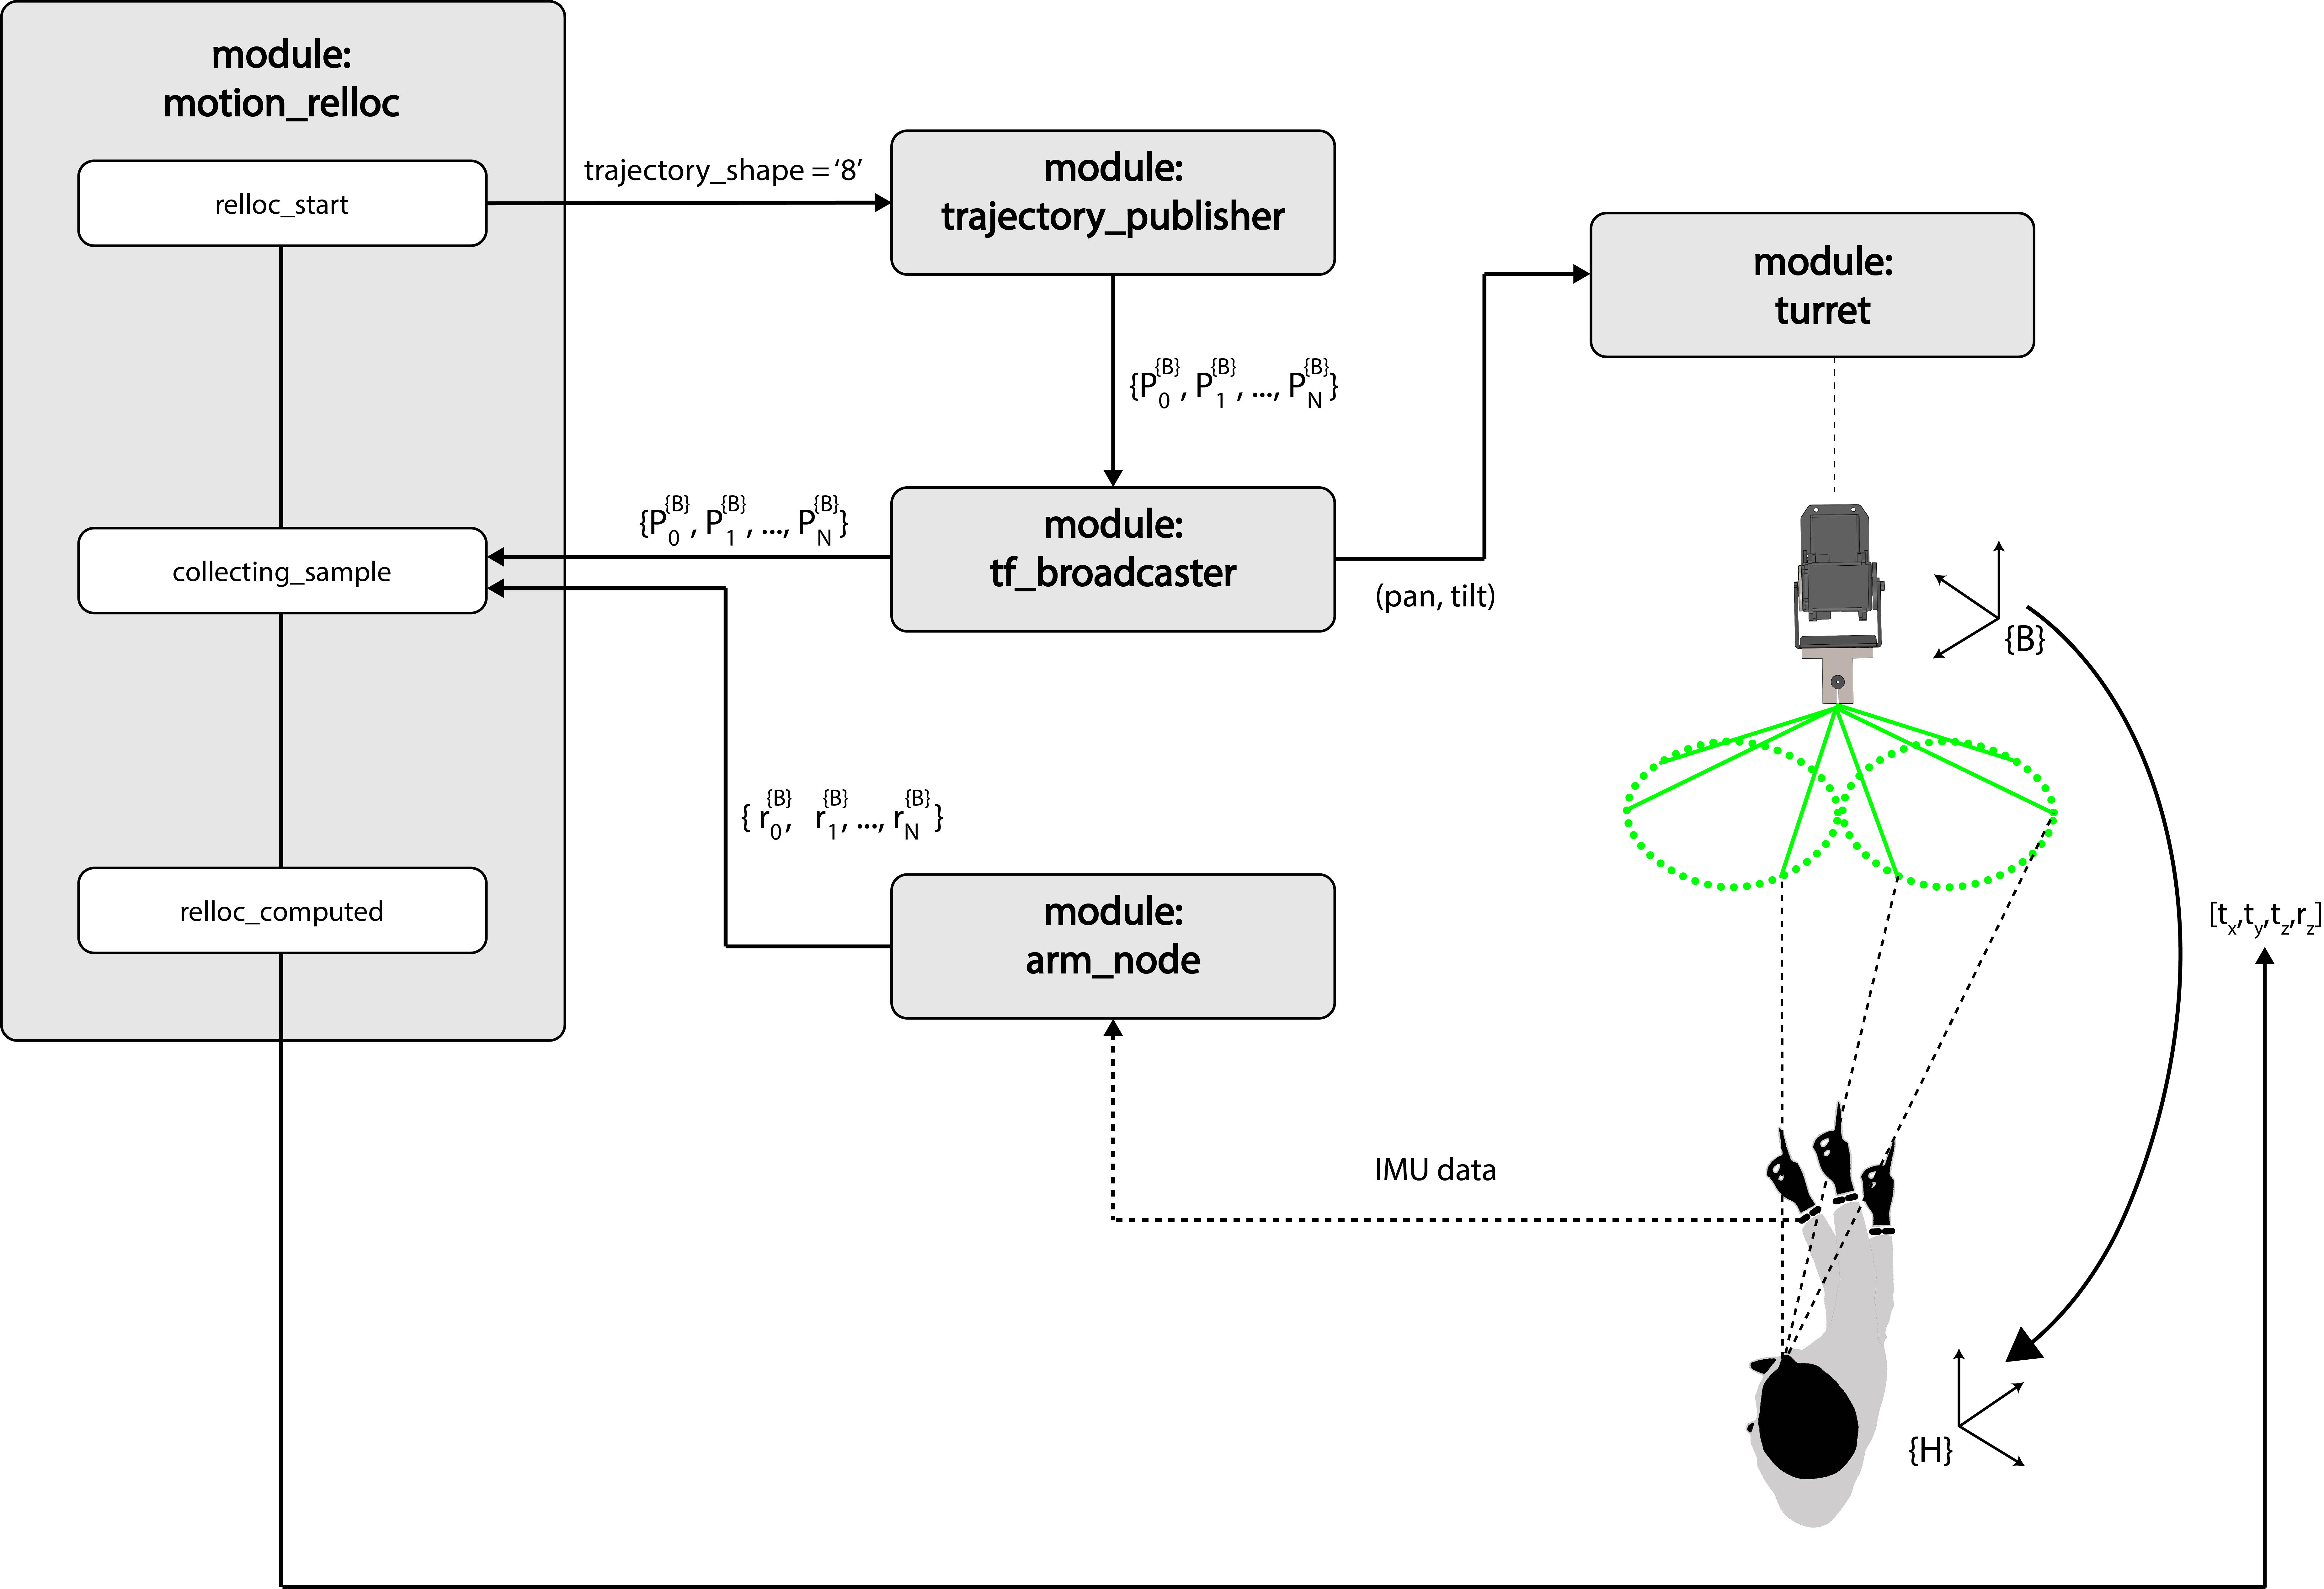
\includegraphics[width=\textwidth]{img/systemPipeline.png}%
	\caption{System Complete Pipeline}
	\label{fig:systemBigPicture}
\end{figure}

\section{Demos Implementation}
We have implemented three different demos to show the behaviour of the system and also demonstrate possible use cases. In that section we will discuss only aspects related to the software implementation of those demos. They are presented in depth in \ref{chap:4} 
\subsection{Relloc Demos}
Obviously, those demos are needed to give an example of the relloc. There are 2 different version of it. In both cases, first we compute the relloc, then we have two different behaviour: in one case, we use the estimated position to mark the point where the user is standing with the laser; in the other case, we allow the user to directly control the laser dot position on the floor (we implemented also a wall version) with pointing gestures.\\
In both cases, all we have to do is compute transformation between human and turret frame: in one case just to obtain the human position in the turret frame, in the other to obtain the point the human is pointing in the turret frame. All these transformations needed are easily obtained, as usual, thanks to the \texttt{tf} library for ROS, which played a major role for those demos. As a matter of fact, in figure \ref{fig:rellocDemo} we can see a user driving the laser around pointing at the ground. Since the relative location is known, goal points expressed with pointing rays in frame $\{H\}$ can be transformed into $\{B\}$ reference and thus be used to drive the turret.

To sum up, the module \textbf{relloc\_try} is taking care of all those transformations and easily interfaces itself with our core system.
\begin{figure}
	\centering
	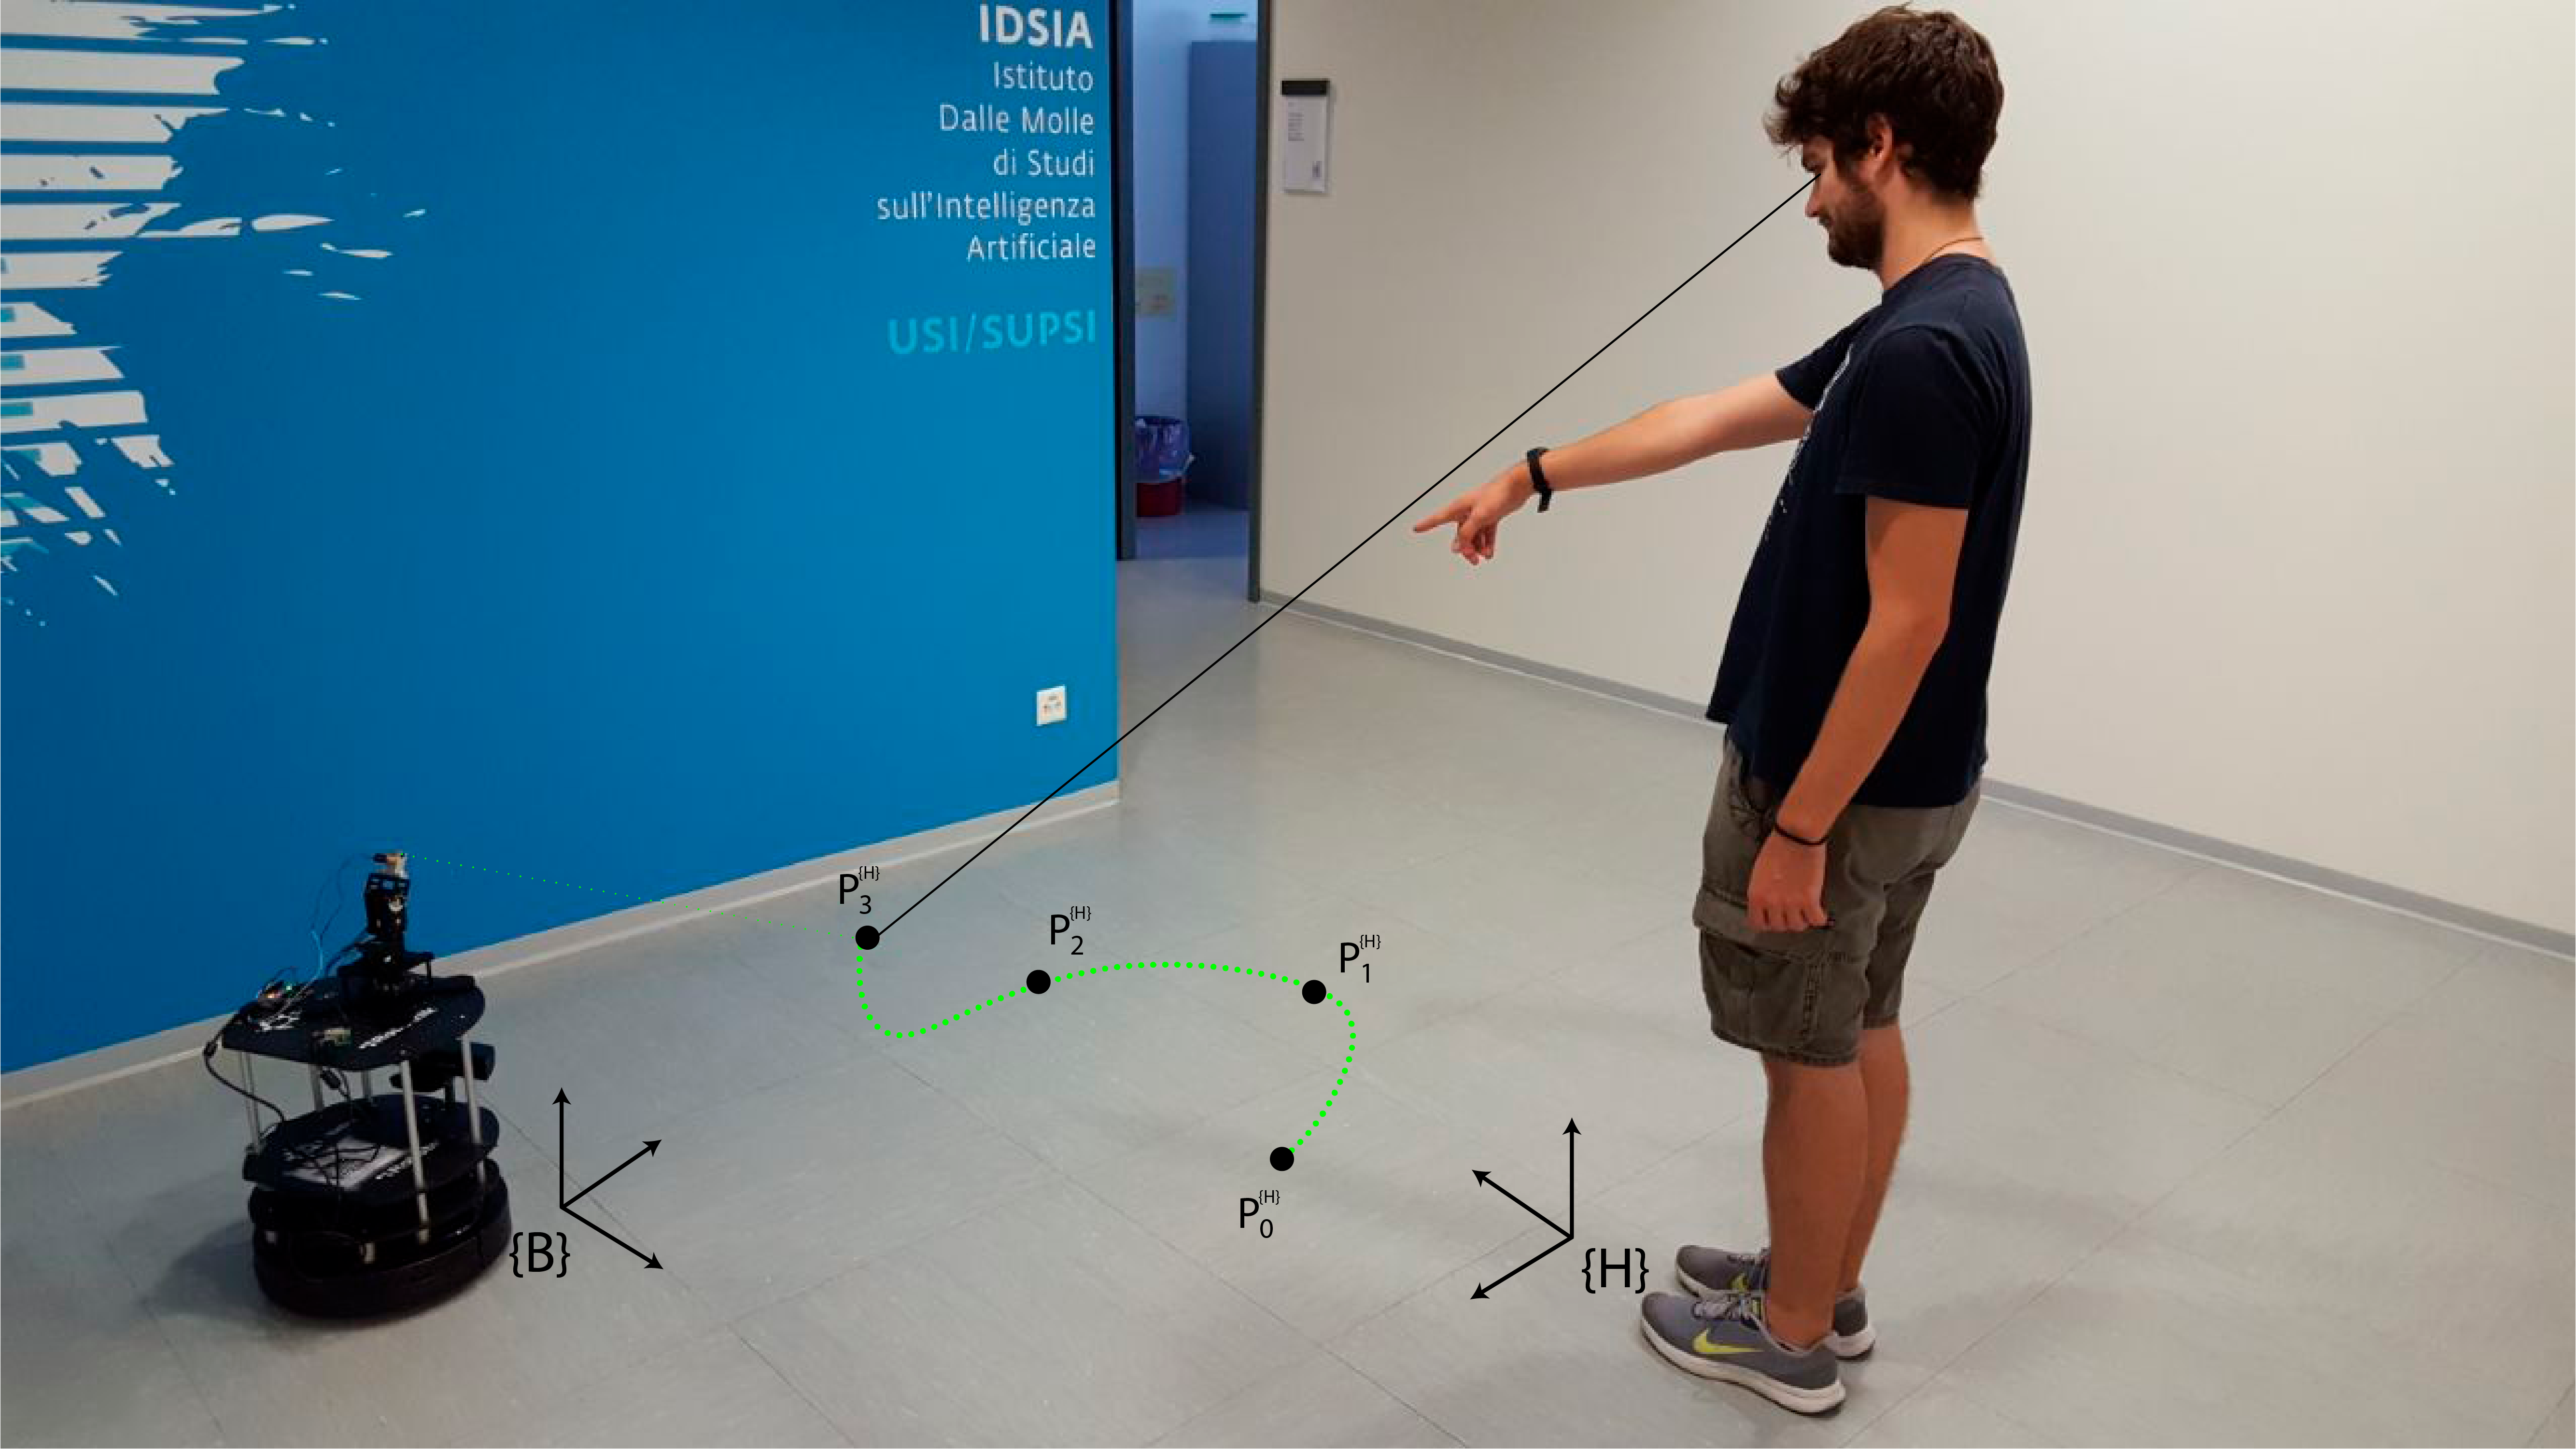
\includegraphics[width=\textwidth]{img/rellocDemo.png}%
	\caption{User Trying the Relloc Demo}
	\label{fig:rellocDemo}
\end{figure}
\subsection{Kobuki Go to Goal Demo}\label{subs:kobukiGoToGoal}
That demo exploits the kobuki platform to show an interesting use case for the system: mobile robot navigation.\\
In that case, we do the relloc and then tell the kobuki to reach a certain position by pointing at it for three seconds.\\
In addition to the relloc system, we implemented a basic PID controller to move the kobuki. The library to interface with the robot is available online \cite{kobuki:ROS}.\\ Moreover, To detect the fact that the user is pointing the same point for three seconds, we implemented a nice function with a fixed size queue where we store the coordinates of the last 150 laser points (which means points in the last $3$ seconds at $50Hz$). We check if the average distance of each point from the first point in the queue is within a given threshold: in that case we detect the 3 seconds pointing.\\
All that additional code is contained in the \textbf{kobuki\_go\_to\_goal} module, which interfaces flawlessly with our system.
\begin{figure}
	\centering
	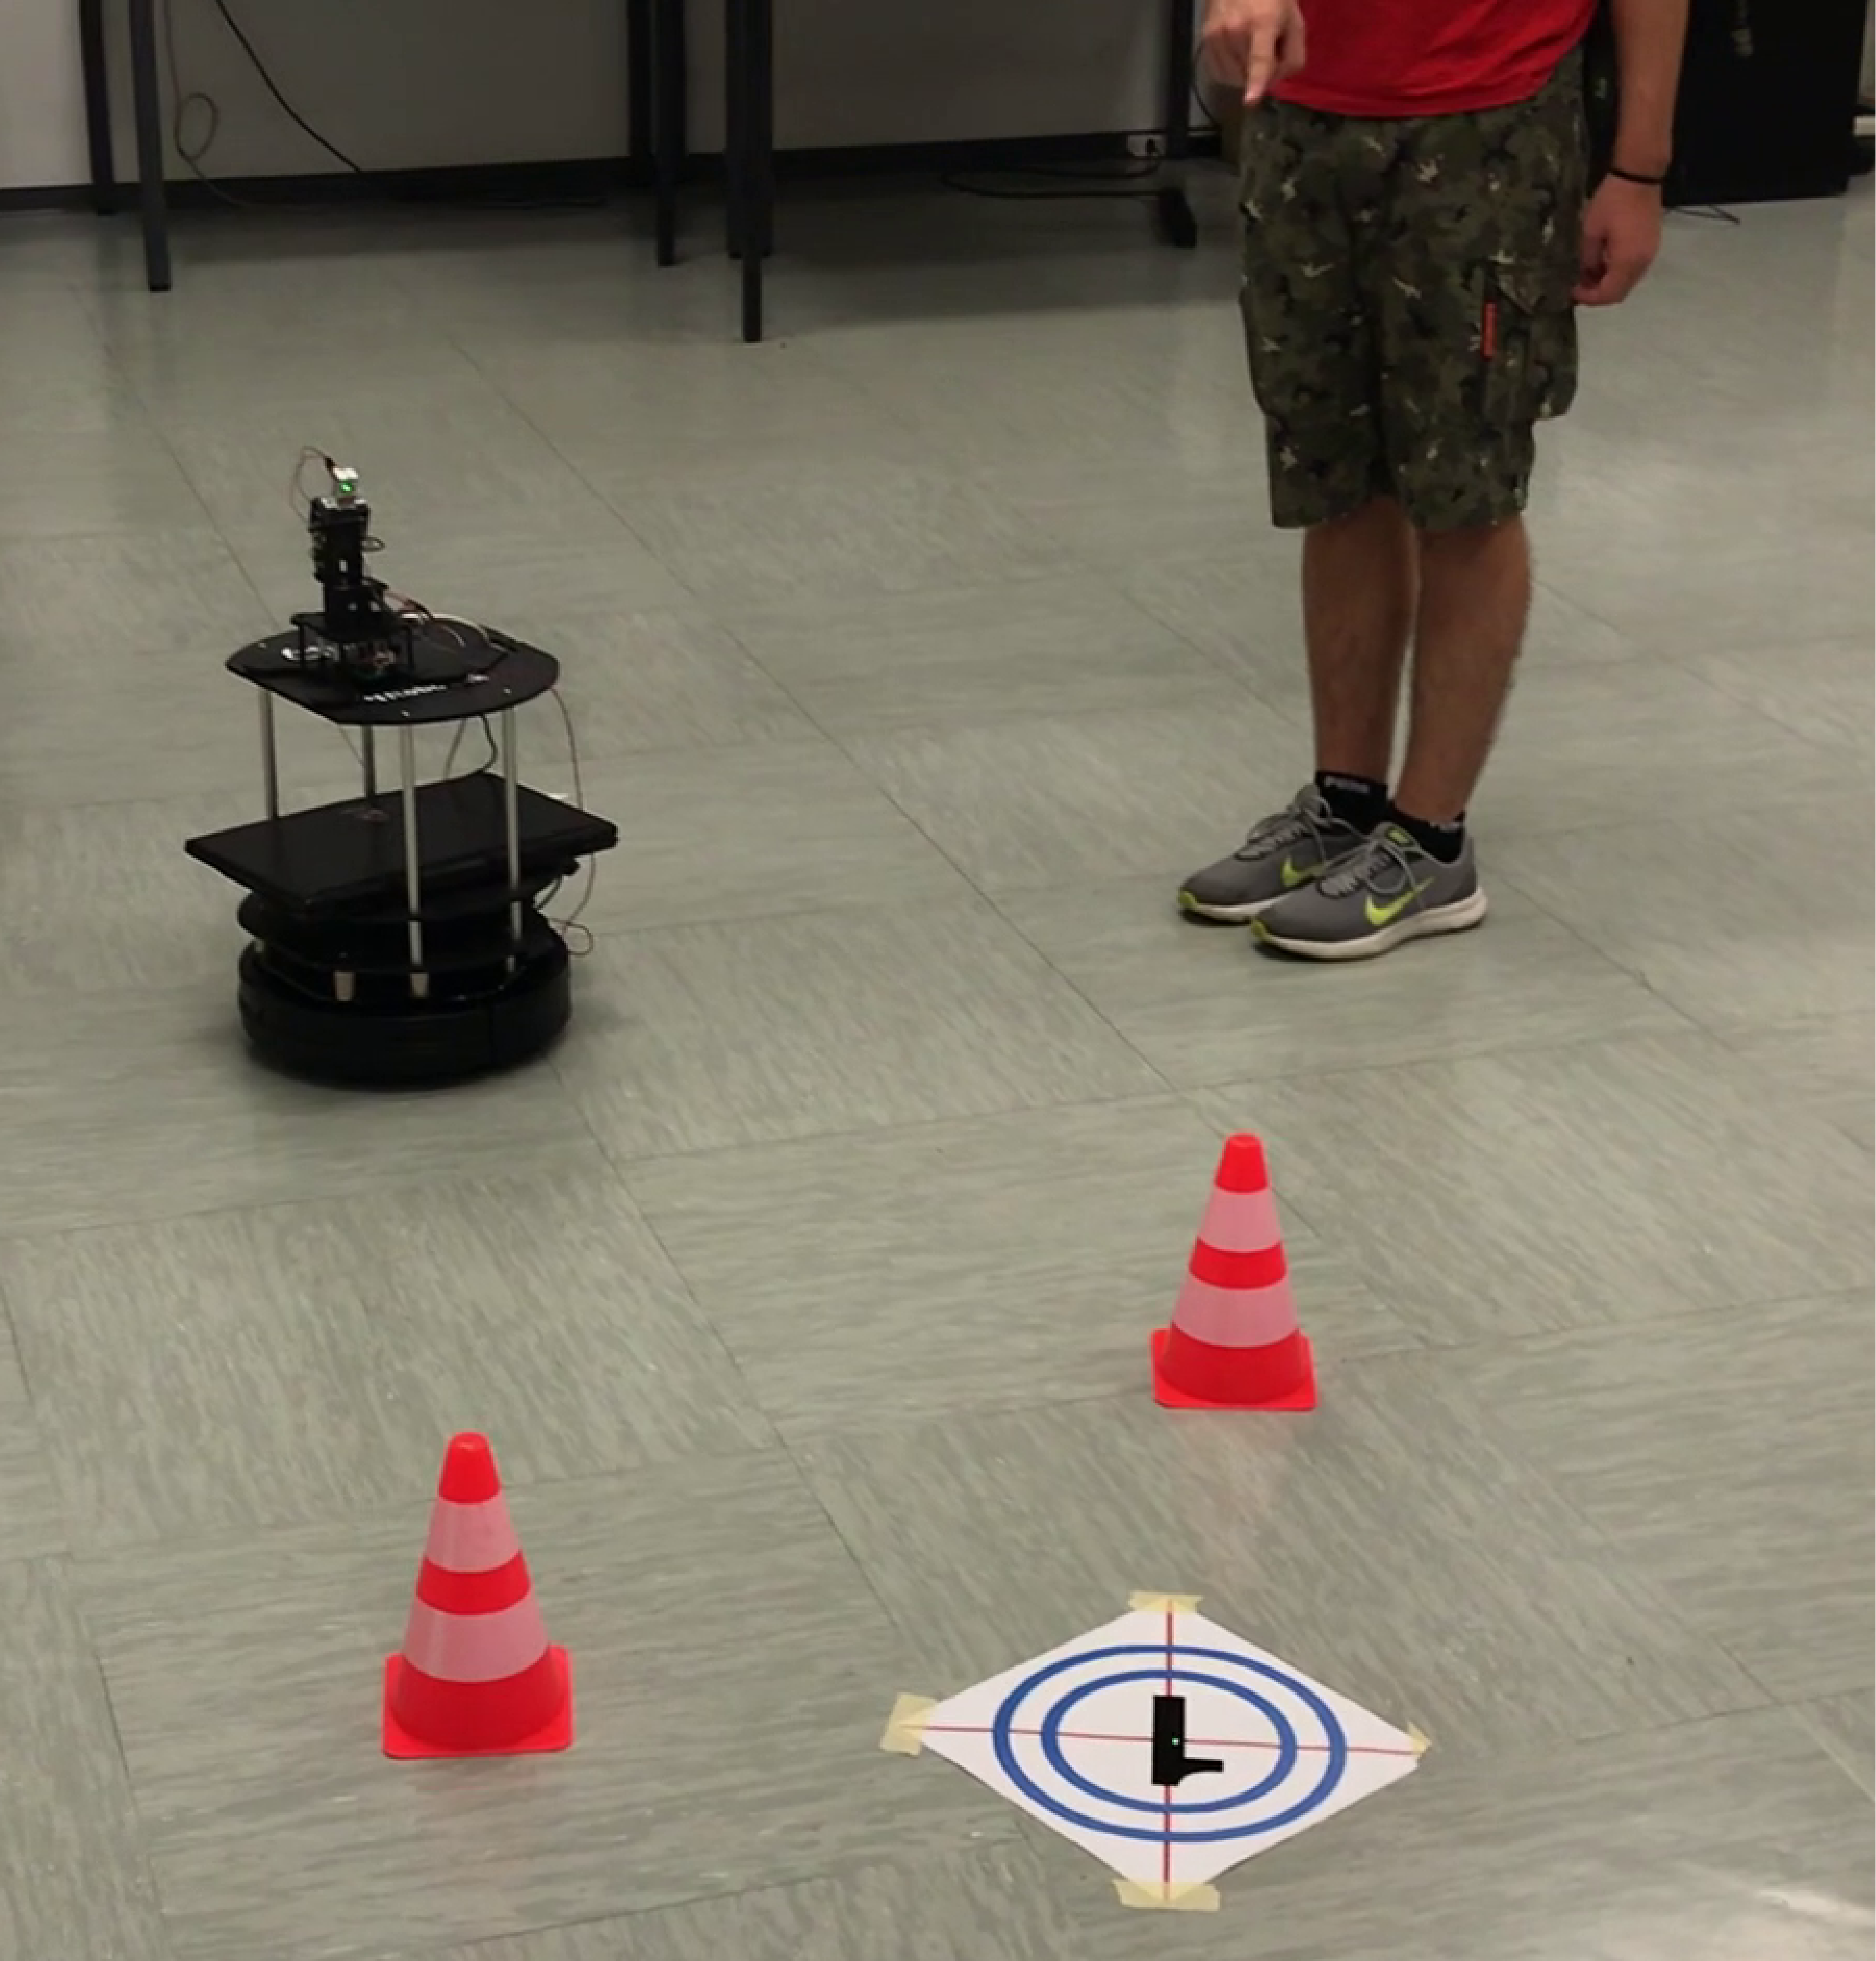
\includegraphics[width=\textwidth]{img/goToGoalDemo.png}%
	\caption{Kobuki Go to Goal Demo}
	\label{fig:goToGoalDemo}
\end{figure}
\subsection{Kobuki Follow Trajectory Demo}
In that case we have the same ingredients of the \emph{Go to Goal Demo}, but the last part is different. Now the kobuki will not simply go to a goal point, but rather it will follow a trajectory drawn by the user.\\
To mark the begin of the trajectory, the user points the start point for three seconds. After an audio feedback, he draws the trajectory with pointing gestures and finally marks the end of it again with another three seconds pointing.\\
The three second pointing detection code is the same explained in \ref{subs:kobukiGoToGoal}. Moreover, we added code to sample the trajectory point list based on distance: that means that the actual trajectory followed by the kobuki is composed of points which are at a threshold distance from their predecessor. Of course, if that threshold is zero, we are using all the sampled points.\\

\begin{figure}
	\centering
	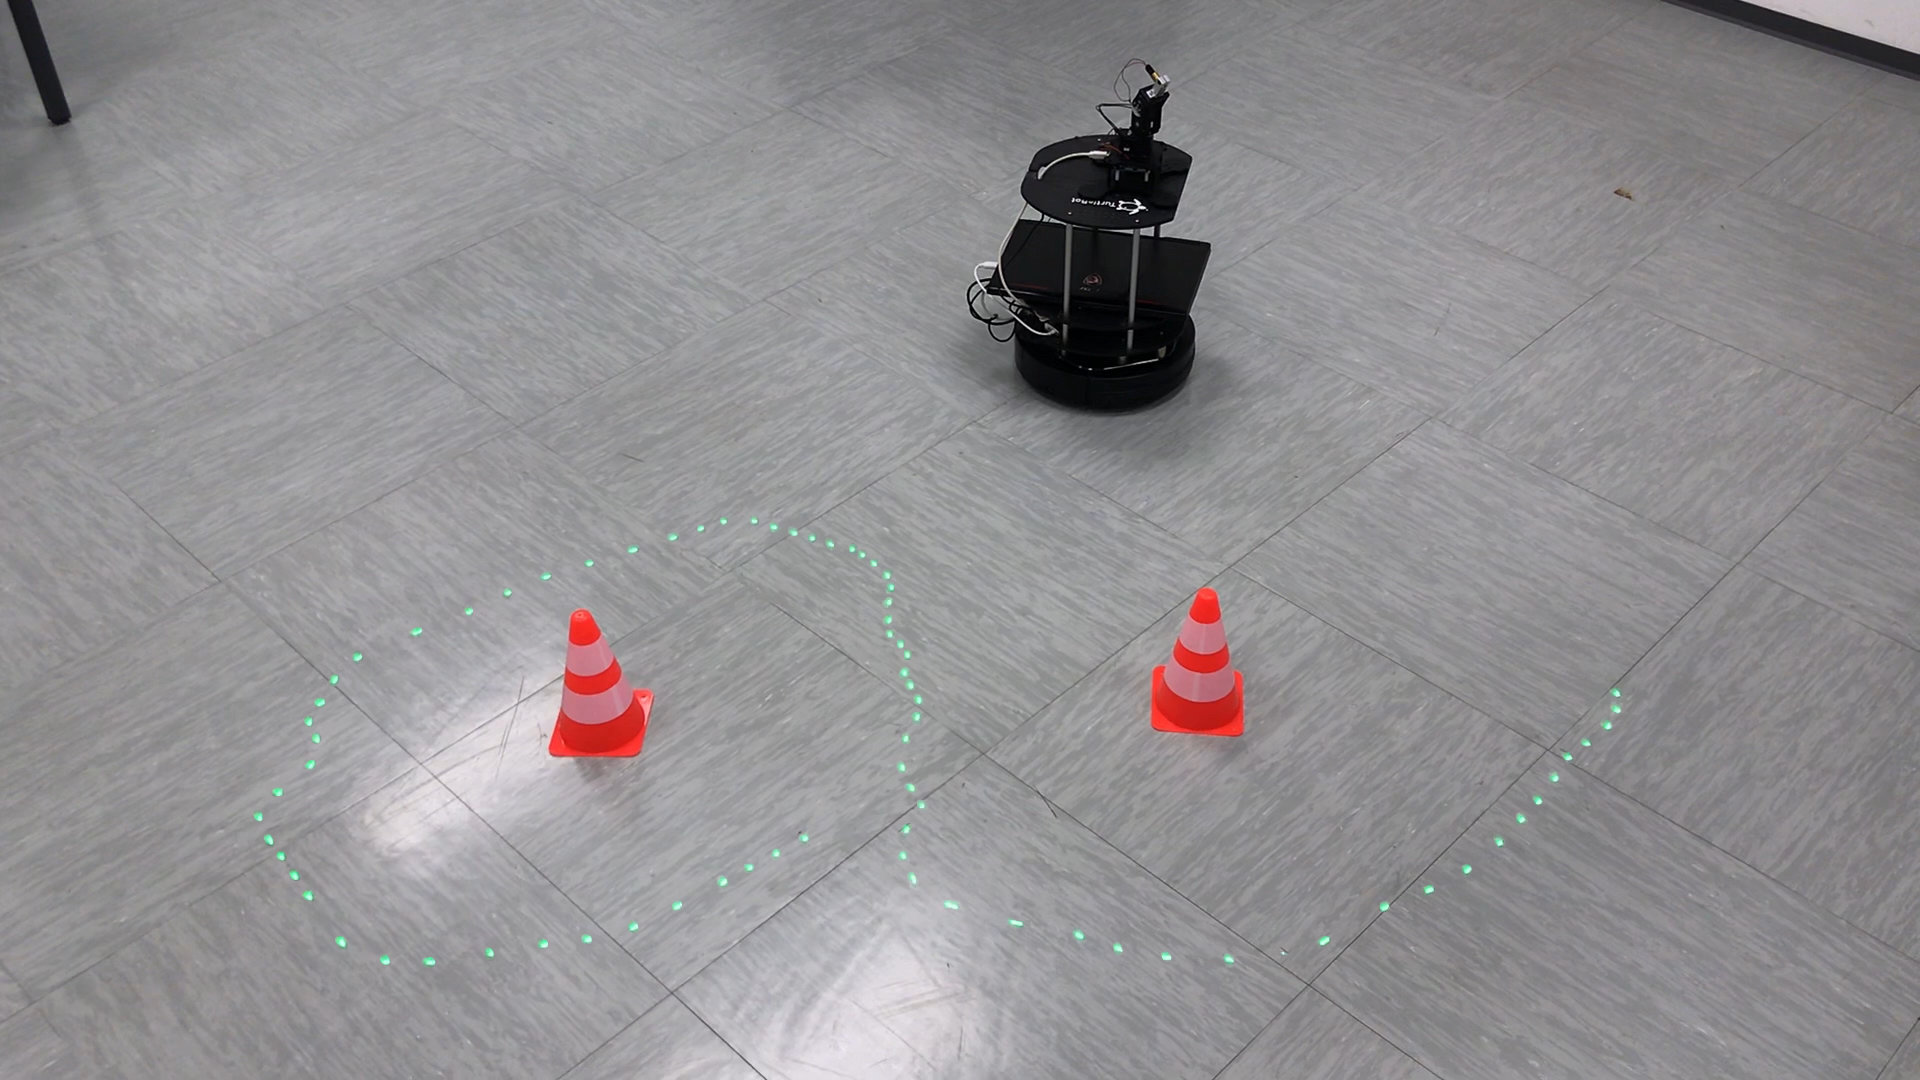
\includegraphics[width=\textwidth]{img/followTrajectoryDemo.png}%
	\caption{Kobuki Follow Trajecotry Demo}
	\label{fig:followTrajectoryDemo}
\end{figure}

\chapter{Experiments and Applications}\label{chap:4}
In this chapter describe the two main experiments we built to collect data and analyze our system. Ten people were involved in the data collection. Each experiment will be presented in terms of goals, procedures and results. Moreover, we will show a couple of applications for the system involving also a ground robot. Those applications are not only discussed, but also demonstrated with a kobuki, allowing us to draw qualitative results.
\section{Pointing Feedback Experiment}
\subsection{Setup}
\begin{figure}
	\centering
	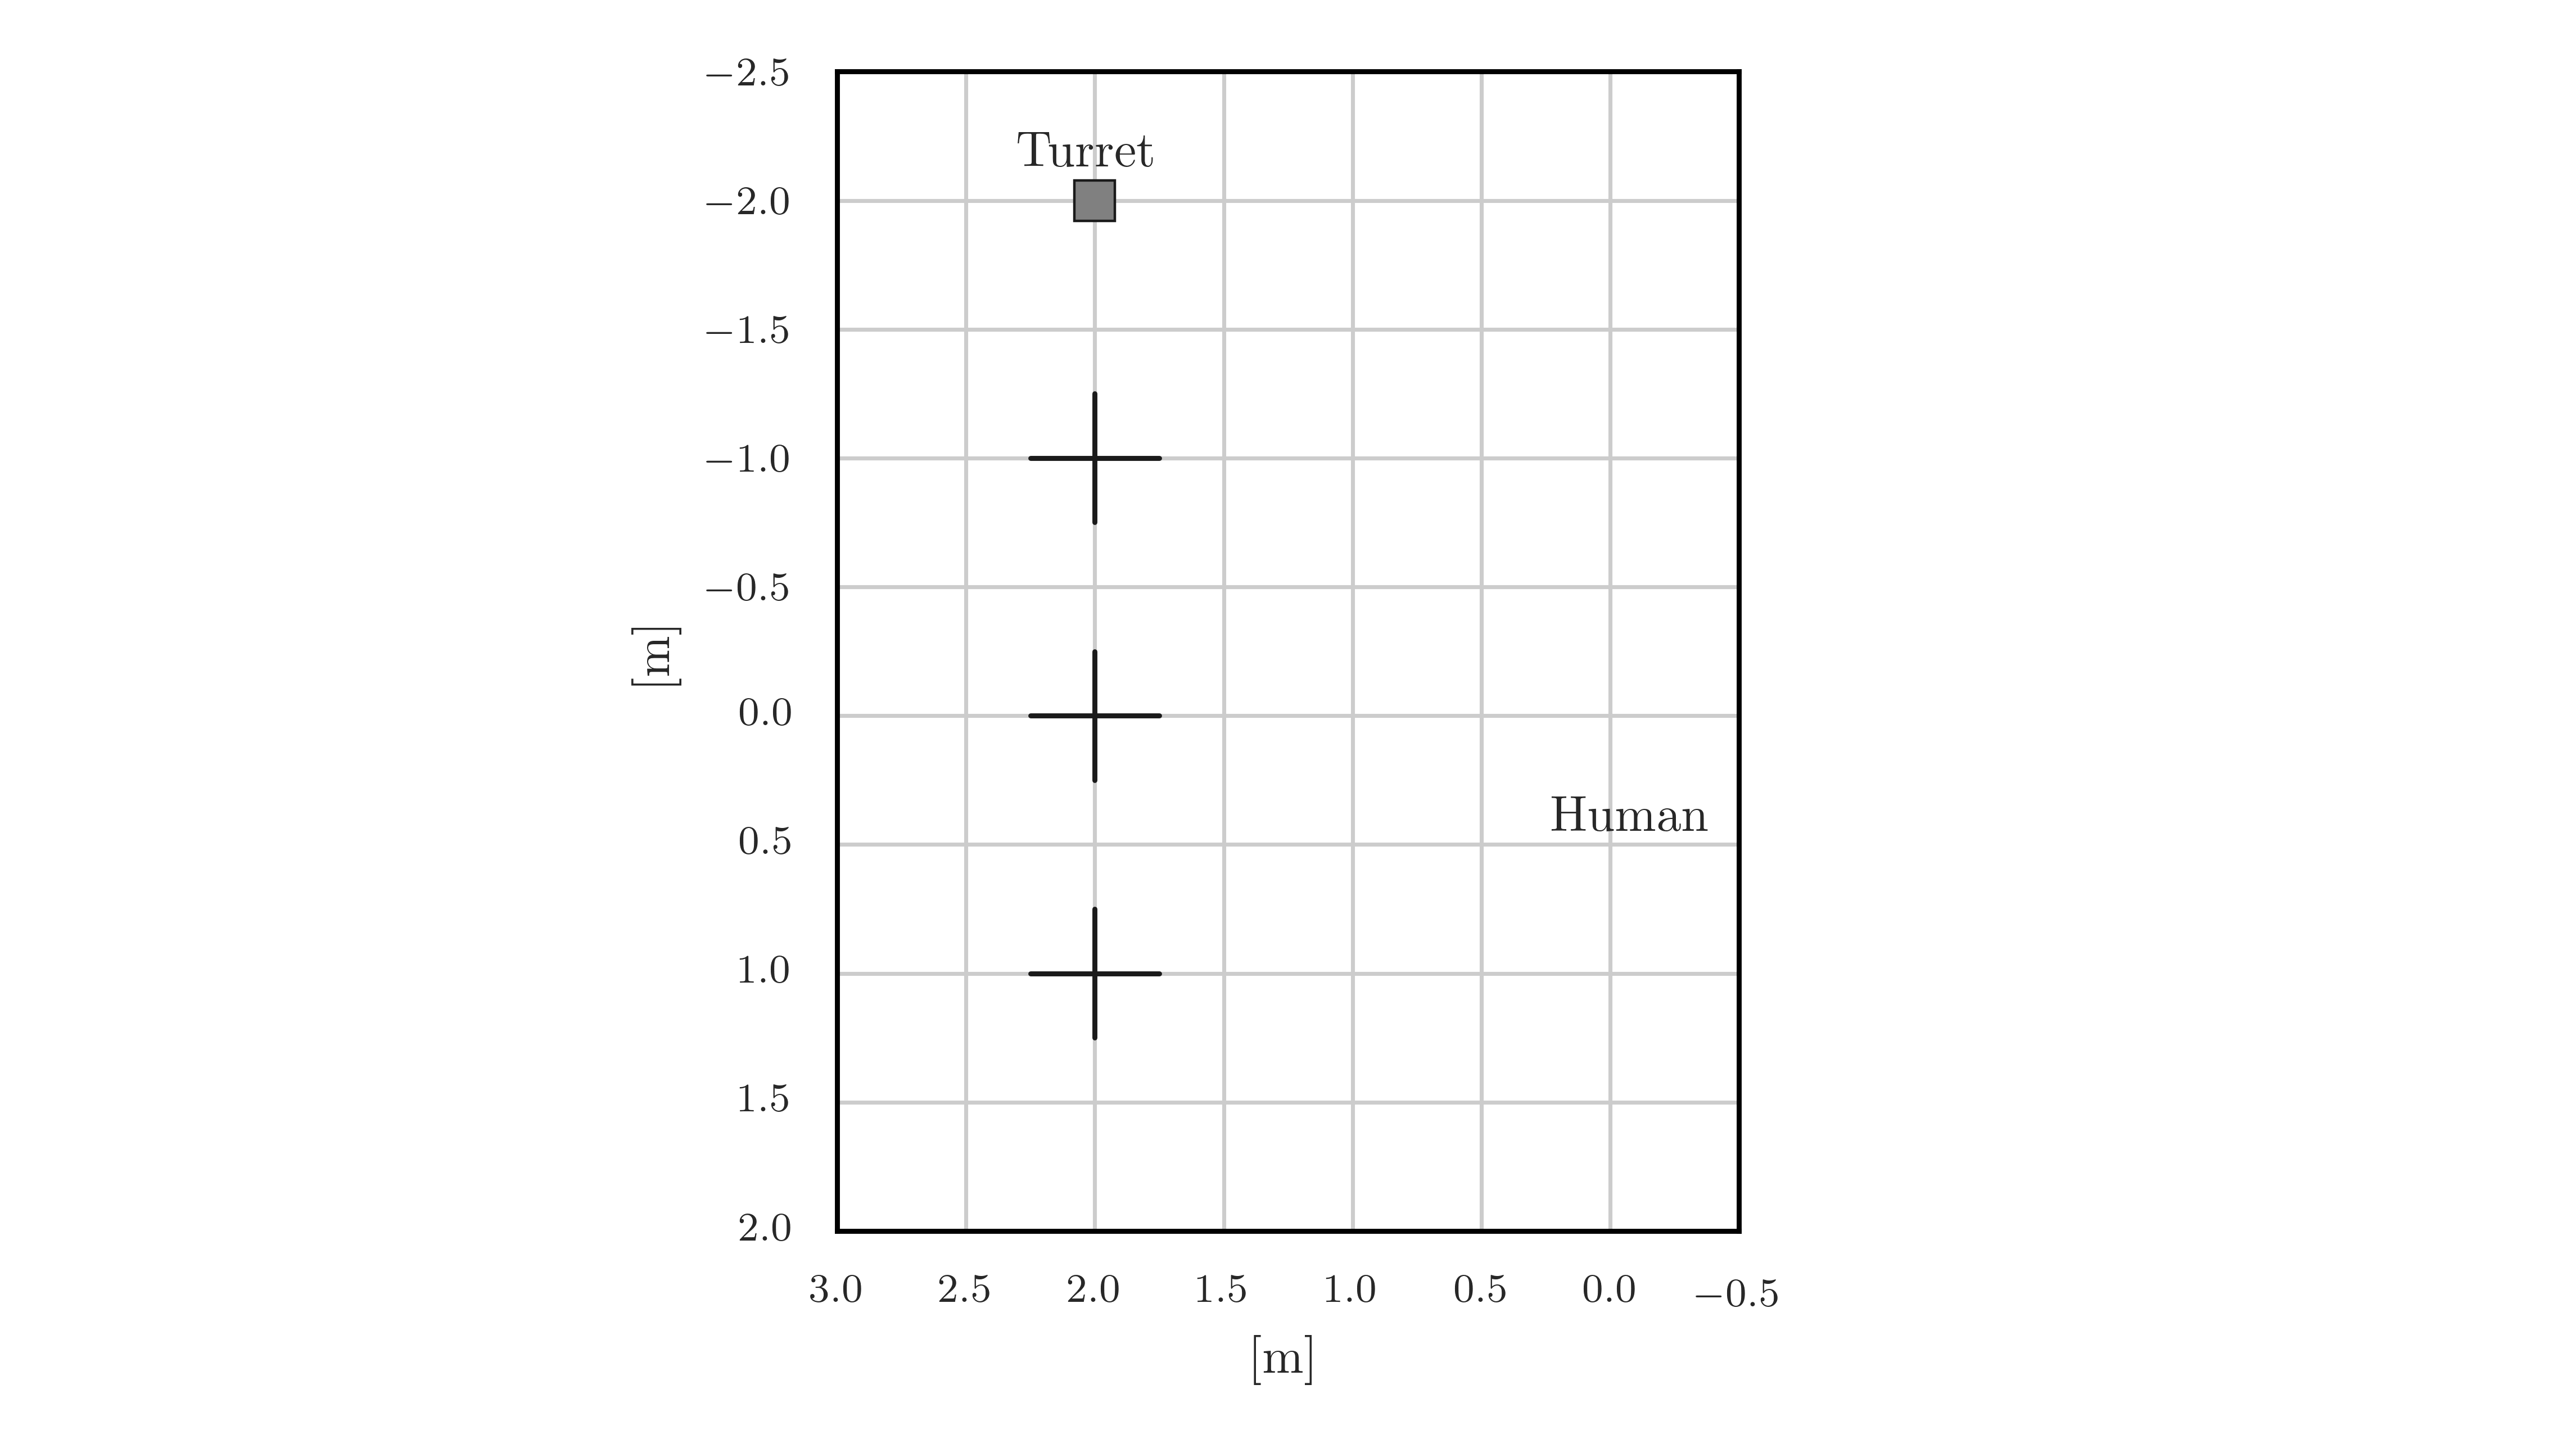
\includegraphics[width=\textwidth]{img/pointingExpSetup.png}%
	\caption{Pointing Experiment Setup (Black Crosses Are Ground Targets)}
	\label{fig:pointingExpSetup}
\end{figure}
We place the turret and three ground targets in known positions. The user is placed in front of the second target, oriented perpendicularly to the line connecting the targets. Figure \ref{fig:pointingExpSetup} shows that setup. The relative localization between the human and the turret is known a priori, so we are not performing any relloc. The user is wearing the IMU and we are collecting his pointing data.\\
The user has to point each target first without any additional visual feedback, so he has to rely solely on his perception. Second, he has to point again with the visual feedback provided by the laser dot. Those are the steps composing each iteration of the experiment (one for each target):
\begin{itemize}
    \item after a countdown, the user points the target without feedback;
    \item the user keeps pointing for 5 seconds;
    \item after a sound feedback, the user can rest his arm;
    \item after a countdown, the user points the target with the laser; feedback;
    \item the user keeps pointing for 5 seconds;
    \item after a sound feedback, the user can rest his arm.
\end{itemize}
Each user has to perform that loop three time for each target, for a total of nine iterations.
\subsection{Goals}
The performance of the interface crucially relies on operator’s perception. Due to simplifications in the pointing model that we use and various sensory errors, the estimated frame transformations and the pointing are expected to be imprecise.\\
With that experiment we want to understand if availability of visual feedback is useful and thus improves the pointing accuracy. This is why we ask users to drive the laser dot to the target, where the laser dot represents the location where the system thinks the user is pointing. Comparing results with and without feedback, we can understand if providing that feedback helps users to timely adapt to any misalignments.

\subsection{Results}
First, we can look at the users' trajectories with and without feedback in figure \ref{fig:userTrajectories}. We can immediately see that without feedback users go straight to their goal point, but that point, for the system, does not correspond to the target. With feedback, on the contrary, users are able to tell the system to point at the target. This intuition can be see in figure \ref{fig:distanceComparison} and is further confirmed by figure \ref{fig:avgDistance}: without feedback, users quickly reach an average distance from the target of 0.5 m but do not improve any further. When the feedback is provided, distance decreases to almost 0 within 5 seconds. This is expected as the system has intrinsic inaccuracies (for example in the reconstruction of pointing rays) which the user is unable to see and correct. 

This demonstrates that real-time feedback is a key component for our system. This justifies all the work done to build the turret, as, while with fast moving robots (e.g. a drone), the robot position itself can be the feedback, for slow moving machine (e.g. a ground robot) the laser dot represents a valid possibility, as also our demos with the kobuki show.

\begin{figure}
	\centering
	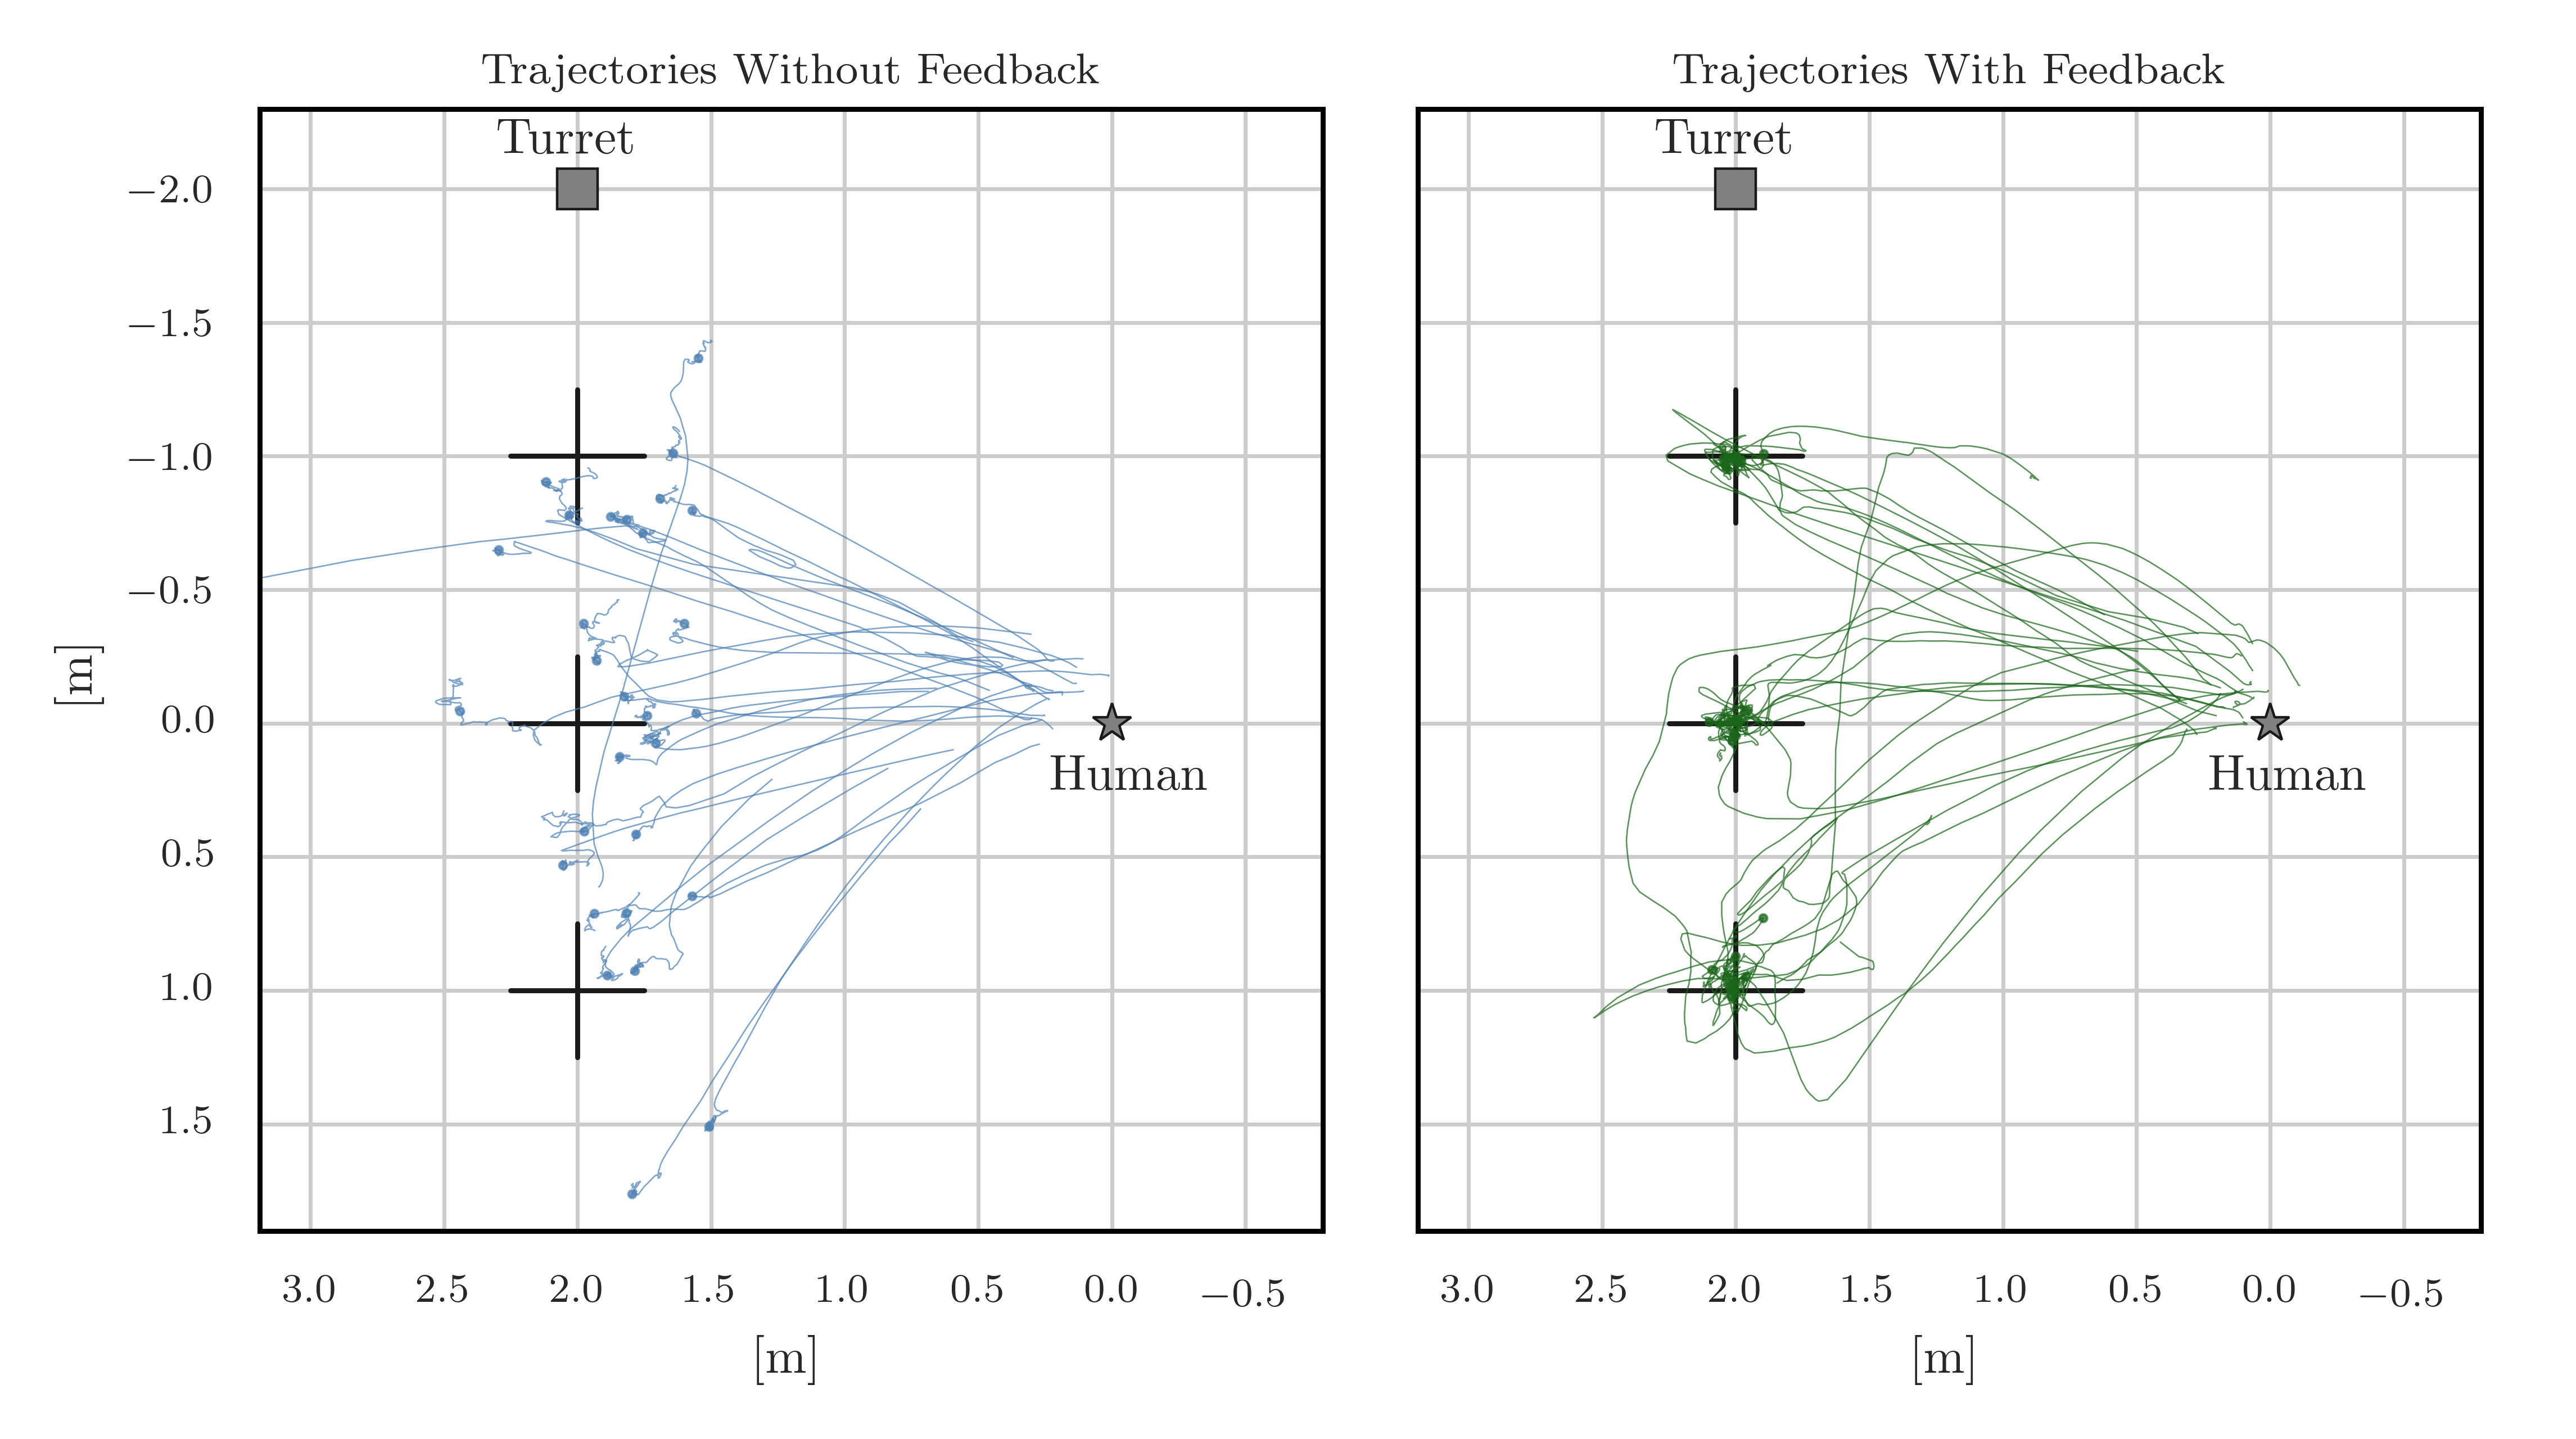
\includegraphics[width=\textwidth]{img/userTrajectories.png}%
	\caption{Users' Trajectories With and Without Feedback}
	\label{fig:userTrajectories}
\end{figure}
\begin{figure}
	\centering
	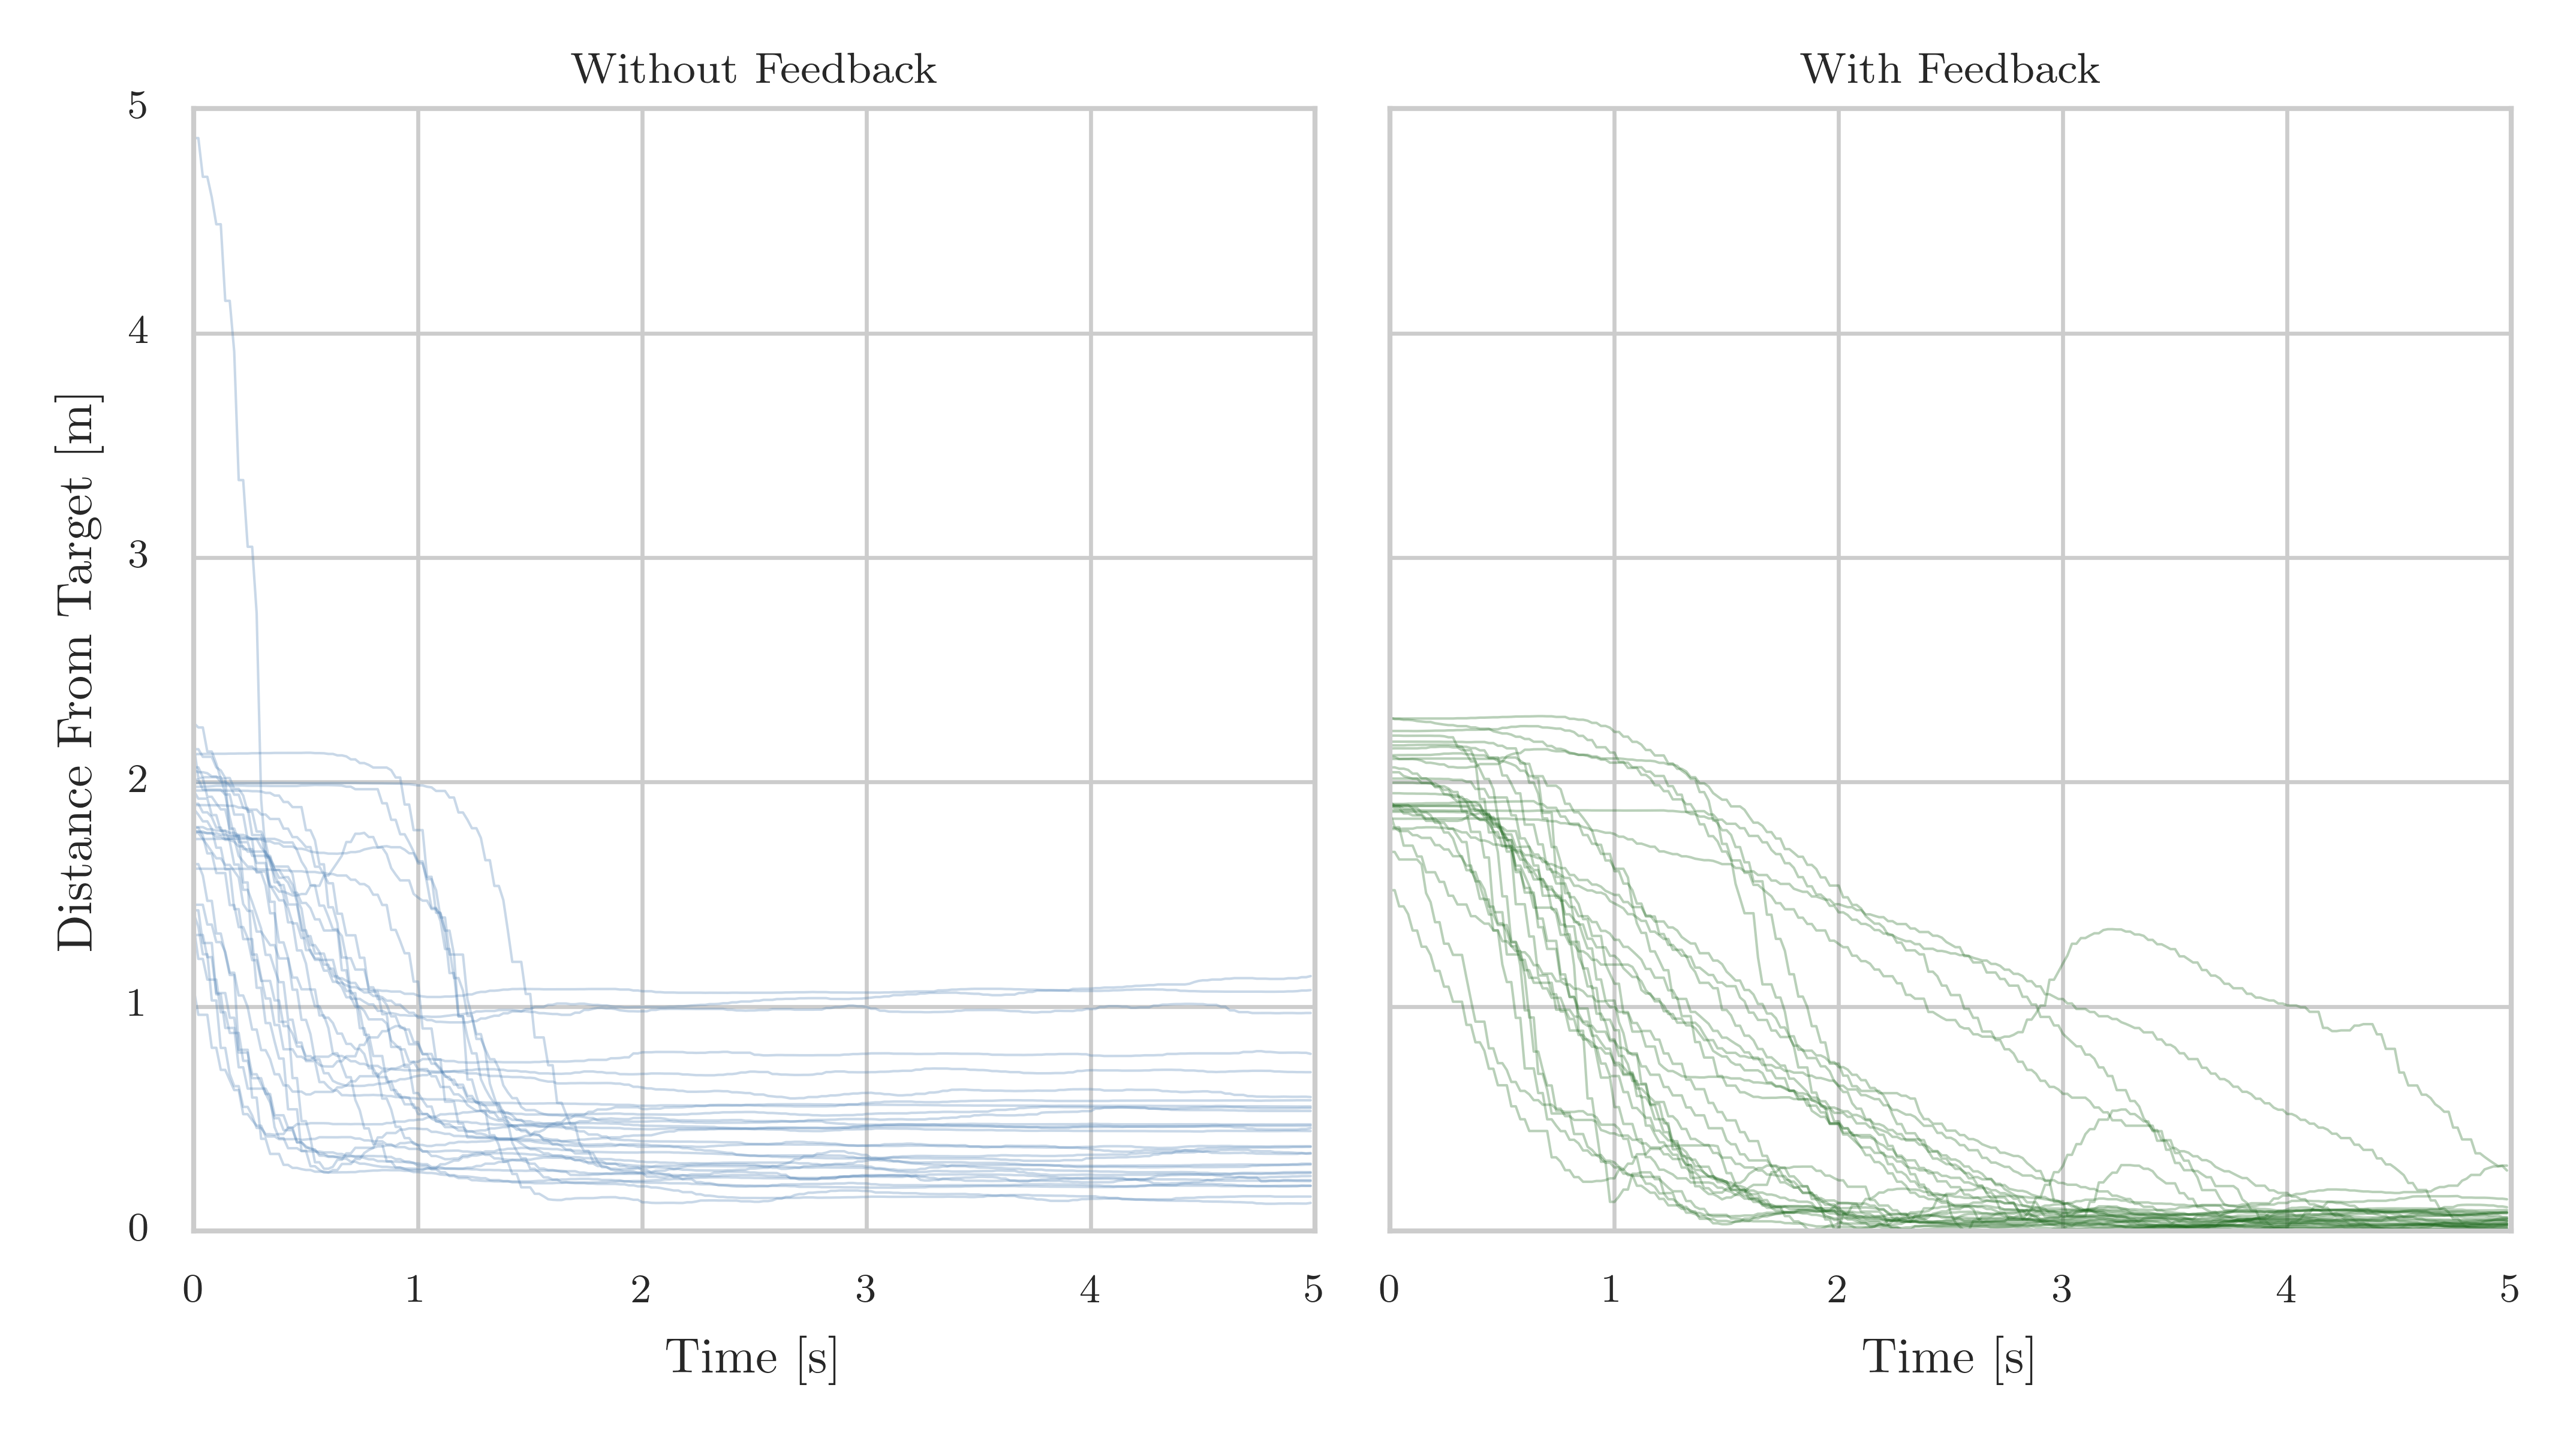
\includegraphics[width=\textwidth]{img/distanceComparison.png}%
	\caption{Comparison Of Distances Over Time}
	\label{fig:distanceComparison}
\end{figure}
\begin{figure}
	\centering
	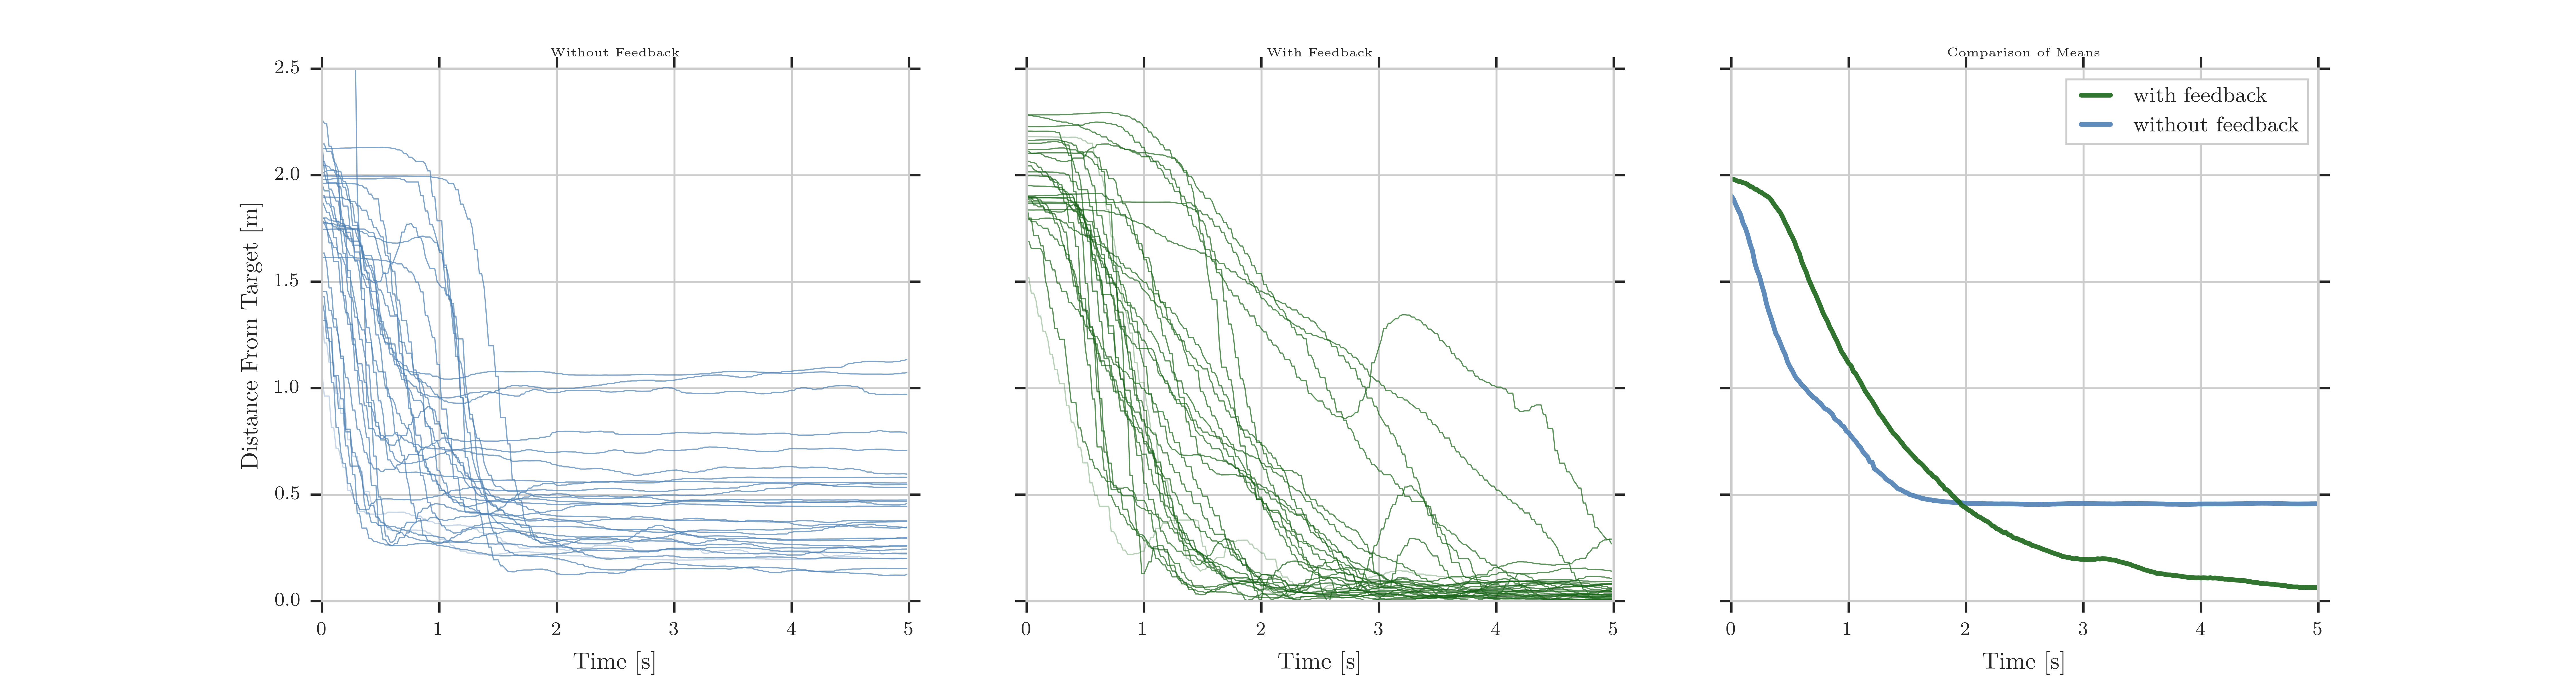
\includegraphics[width=0.7\textwidth]{img/avgDistance.png}%
	\caption{Comparison Of Average Distances Over Time}
	\label{fig:avgDistance}
\end{figure}

\section{Relloc Experiment}
For that experiment we will describe the setup and the goal, but will provide only results obtained with the first turret model, which heavily influenced the results with its limited performance. We have also experimented a bit with the second turret obtaining better qualitative result, but we did not have time to perform an entire data collection with users, which we plan to do in the future.

\subsection{Setup}
We perform the relloc 9 times from 9 different known positions on the floor. The order of the positions is randomly shuffled for each user. So, the experiment runs the following loop 9 time for each user:
\begin{itemize}
    \item the turret points the position where the user must stand and starts a countdown;
    \item at the end of the countdown, the relloc starts: the turret draws the $\infty$ trajectory and the user follow it with pointing gestures;
    \item once the relloc is done, the turret points to the estimated location of the user.
\end{itemize}
In that way we can have an immediate visible the result: the nearer the turret is pointing to the user, the better the relloc is working. We can obtain that measure directly confronting the known initial location with the estimated one.
\begin{figure}
	\centering
	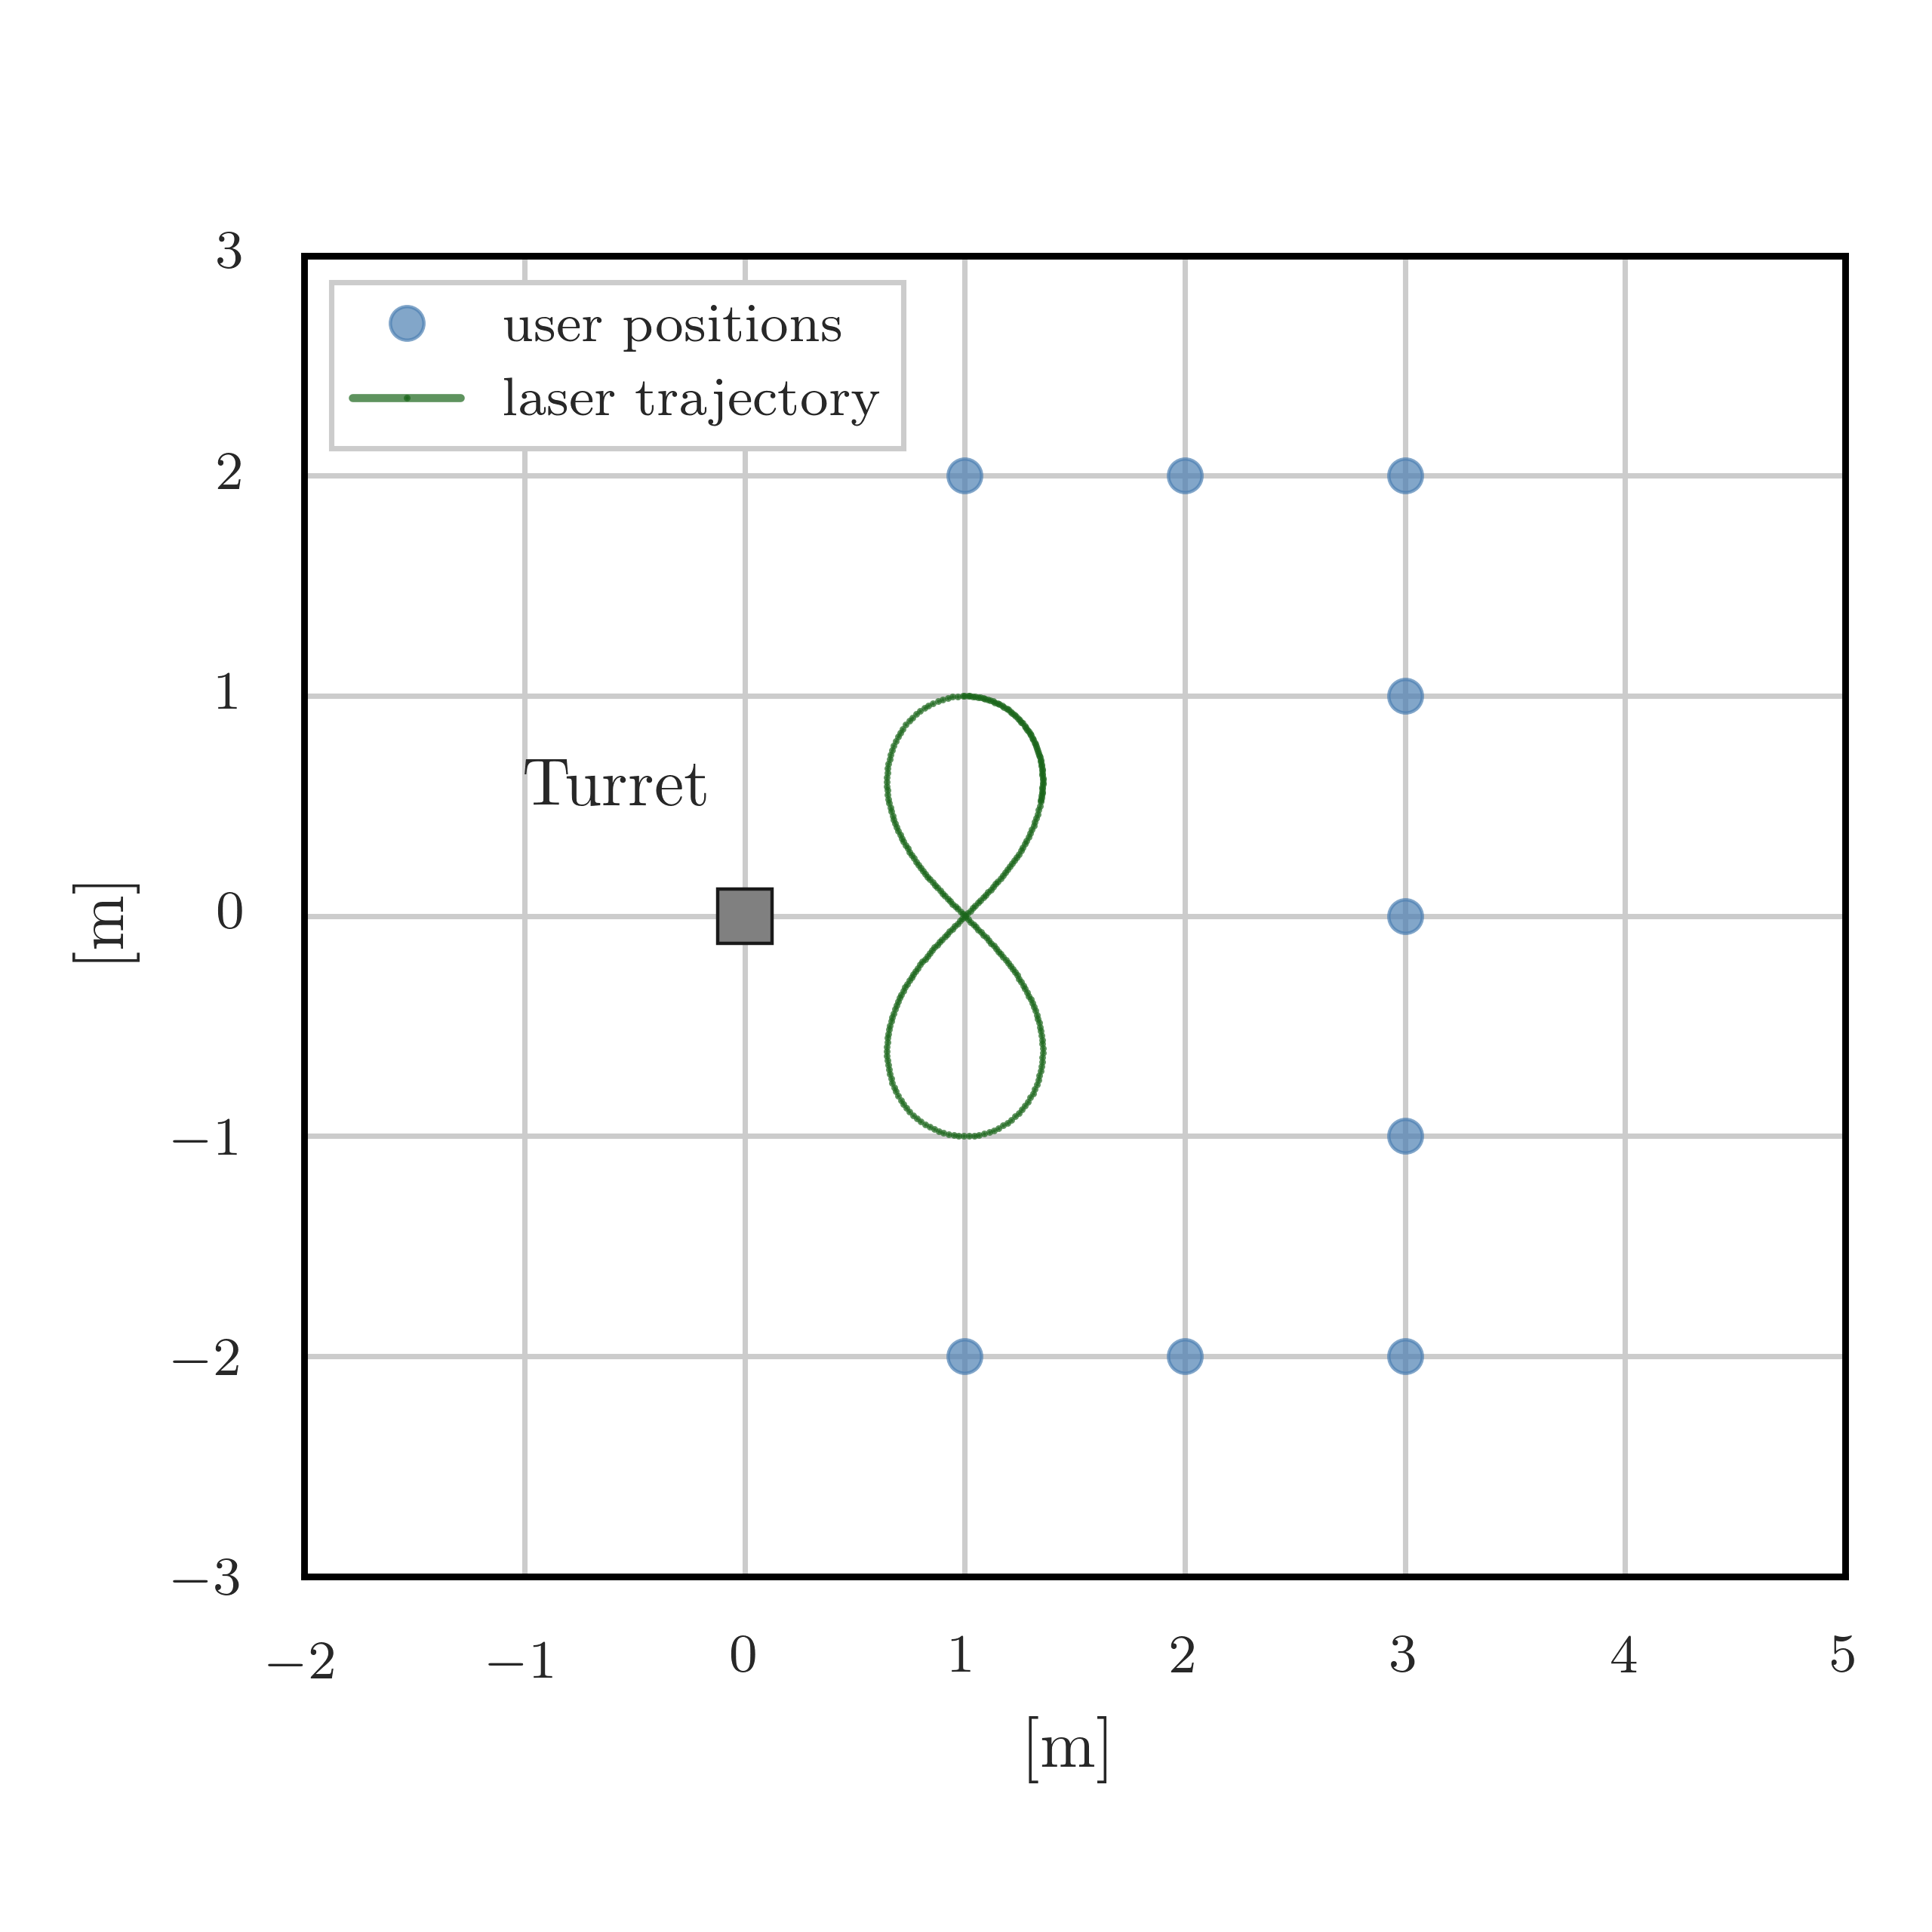
\includegraphics[width=\textwidth]{img/rellocExpSetup.png}%
	\caption{Relloc Experiment Setup}
	\label{fig:pointingExpSetup}
\end{figure}

\subsection{Goals}
The main goals of that experiment of course is to obtain a direct estimate of the relloc precision. Moreover, it is useful to see if also inexperienced users can interface with the system easily.

\subsection{Results}
As already said, we collected data only with the first turret model. We will also run the experiment with the second turret, but from the trials we already did, we have qualitative evidence that the second should obtain better results than the first. \\
However, we report the average error obtained with the data collected with the first turret:
\begin{align}
    \text{mean\_distance\_error} =&\ 48.74\text{ cm} \nonumber\\
    \text{mean\_x\_error} =&\ 36.71\text{ cm}\nonumber\\
    \text{mean\_y\_error} =&\ 24.60\text{ cm}\nonumber
\end{align}
where \textbf{mean\_distance\_error} is the mean of the distances between the position where the user is supposed to be when starting the relloc and the position estimated by our system. \textbf{mean\_x/y\_error} are the means of the differences between each coordinates.

\section{Applications}
As already mentioned, we explored a couple of applications for our system. One consists exactly in what was done for the experiments already presented. In fact, that system is useful to collect data and study pointing models. It also serves as a tool to asses the performances and the precision of the relloc procedure.\\
\begin{figure}
	\centering
	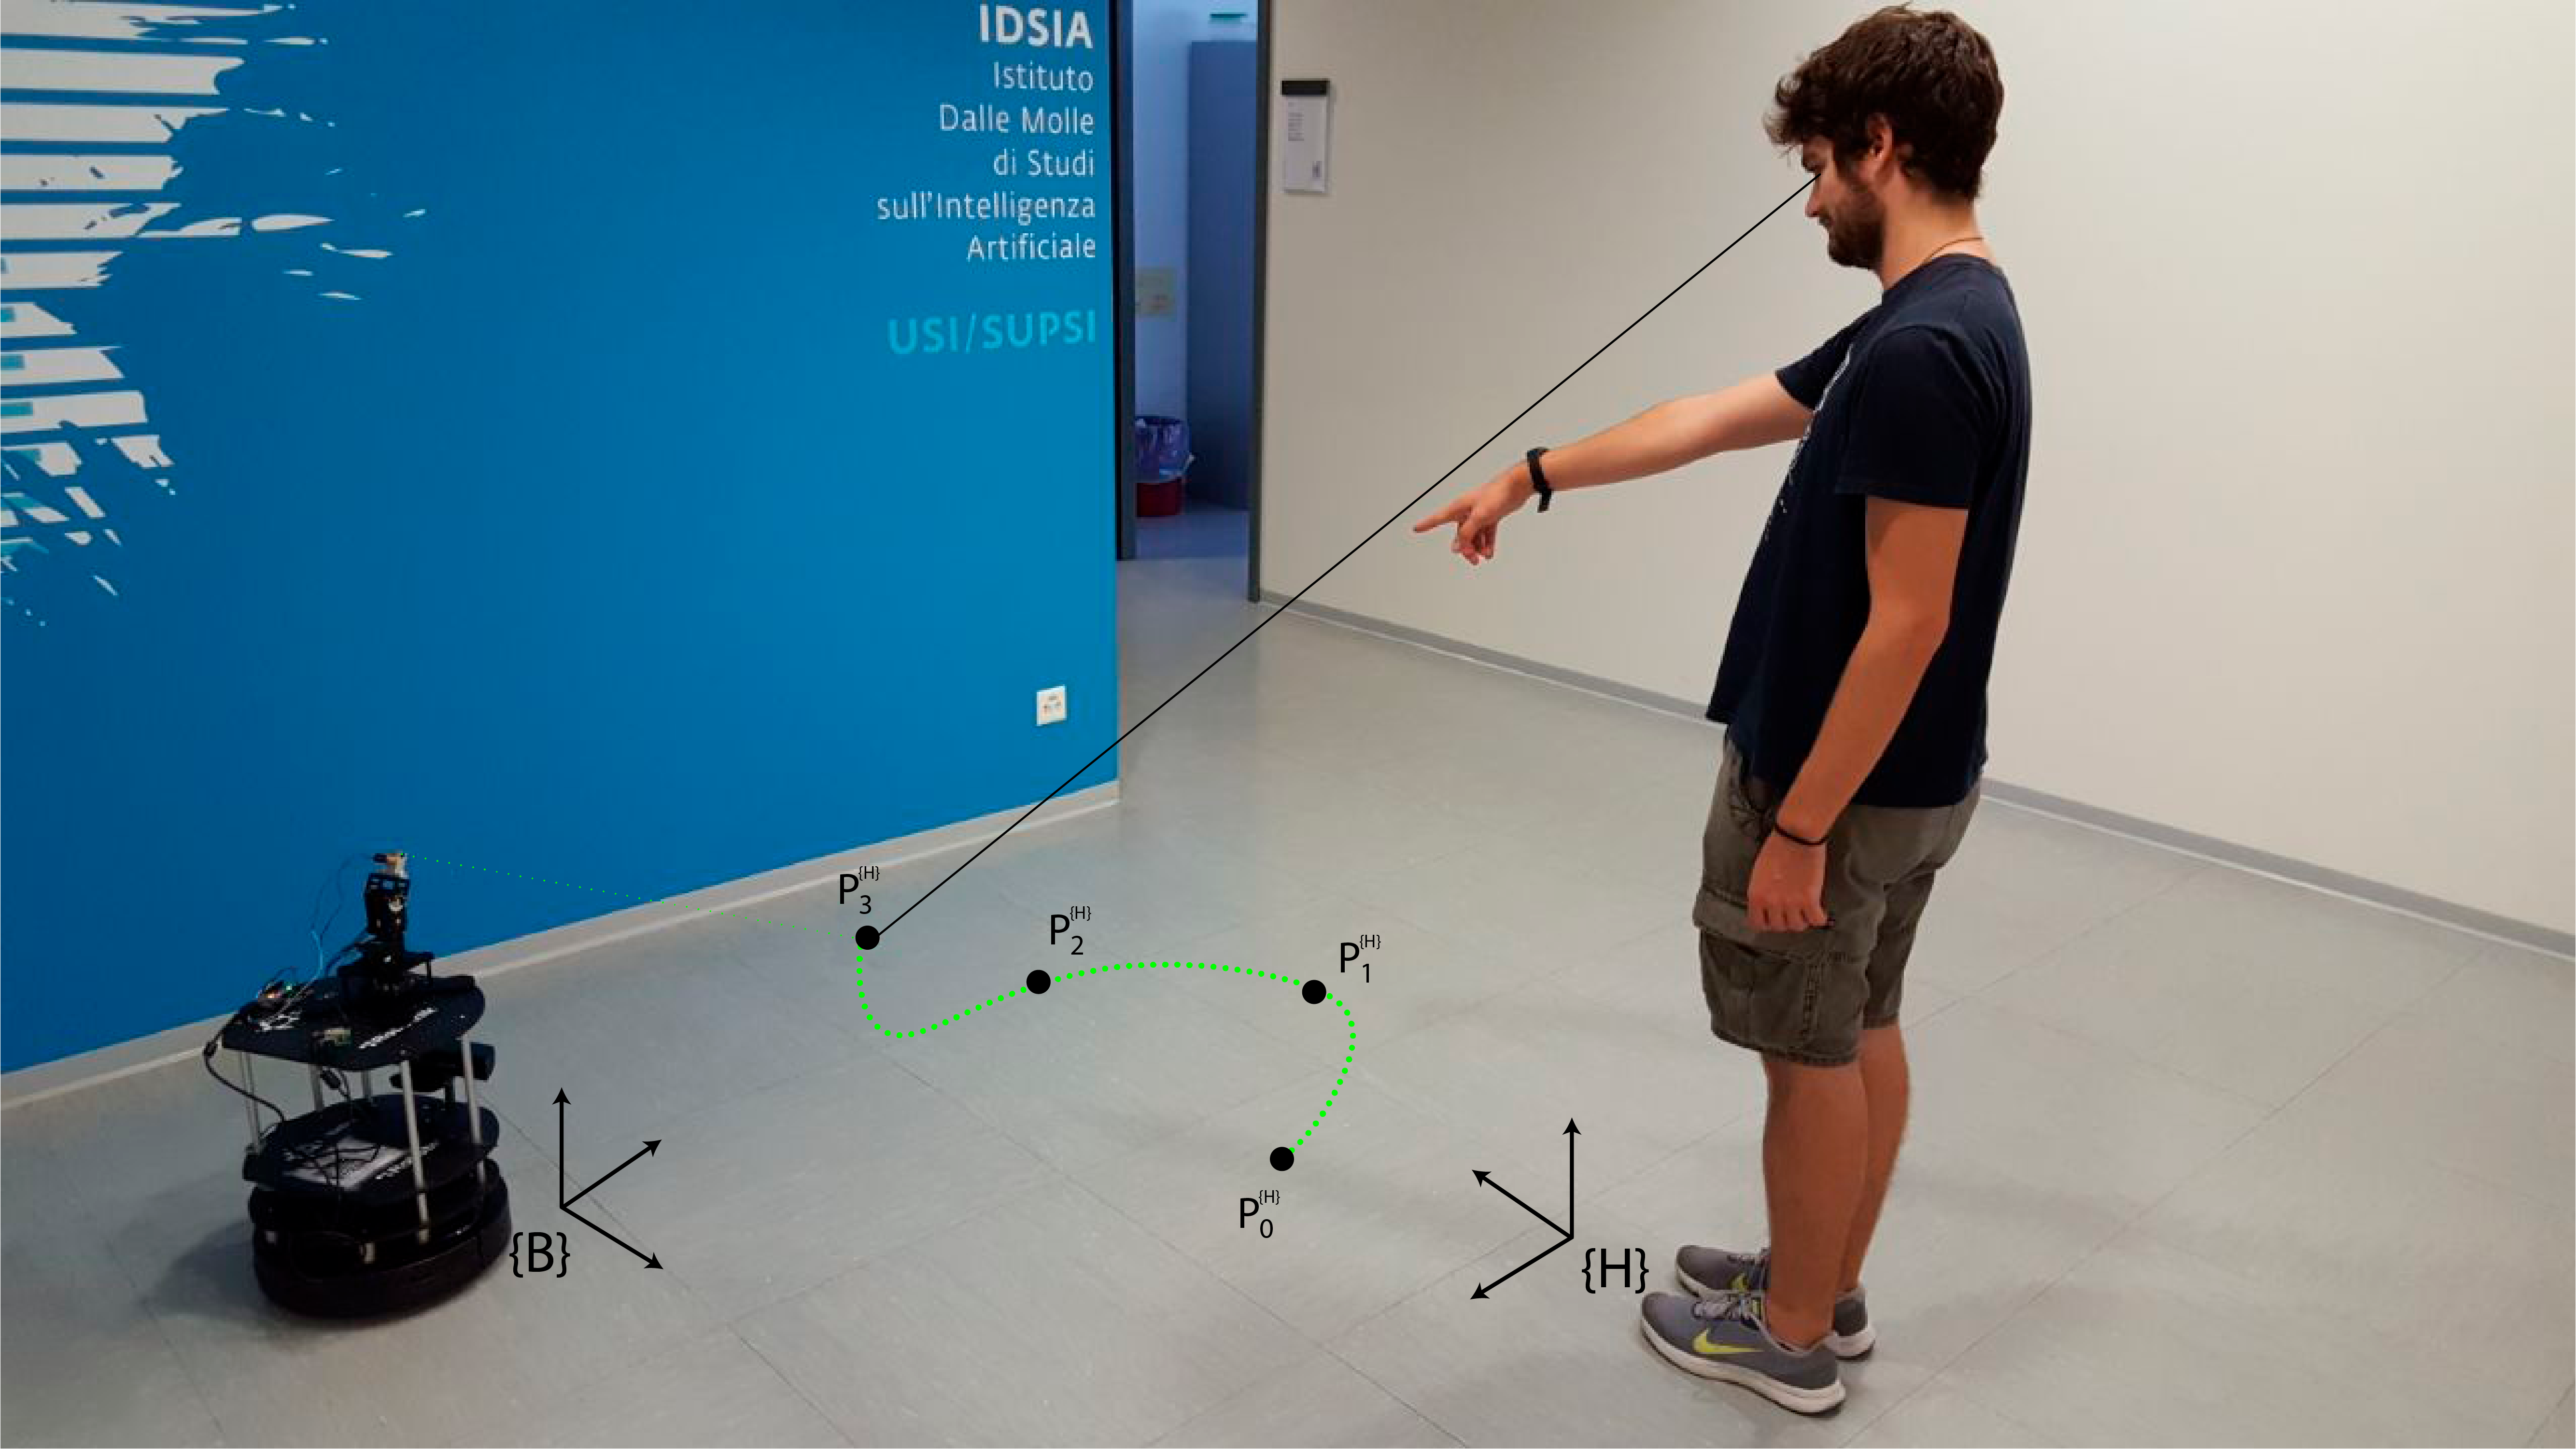
\includegraphics[width=\textwidth]{img/rellocDemo.png}%
	\caption{User Driving the Laser Dot After the Relloc}
	\label{fig:rellocDemoPhoto}
\end{figure}
However, in that section will we present two entire human-robot interaction scenarios involving a ground robot (the kobuki) as well as the turret.\\
A video containing both of them is available at \todo{ref al video}

\subsection{Kobuki Go to Goal Application}
The original relloc system was applied to control a flying robot \cite{gromov2018robot}. In that context, the feedback user had while controlling the drone with pointing consisted of the drone itself. However, that approach is not suitable for a slow moving ground robot, as the kobuki. Here the turret system developed for this thesis comes in play: mounting it on top of the kobuki, we can face the mobile robot navigation task in a convenient way.\\
Figure \ref{fig:kgtgSetup} shows the setup of the demo: we have the user wearing the IMU device and the kobuki equipped with our turret. The steps composing the demo are the following:
\begin{itemize}
    \item the user does the relloc (figure \ref{fig:kgtgRelloc});
    \item an audio feedback alerts the user that the relloc is done and he can now move the laser with pointing;
    \item the user points the place he wants the kobuki to reach for three second (figure \ref{fig:kgtgPointing});
    \item the kobuki moves to that point, while the laser keeps pointing at it. (figure \ref{fig:kgtgGoal})
\end{itemize}
Figure \ref{fig:kgtgGoal} gives also a qualitative feedback: the user is able to drive the kobuki through the cones easily and precisely.
\subsection{Kobuki Follow Trajectory Application}
Here we add another step to the previous go to goal application: now, by pointing for three seconds, users mark the begin of a trajectory. Then, they can draw an entire trajectory (figure \ref{fig:kftTrajecotory} and finally, pointing again the same point for three seconds, set the end point. After that, the kobuki will follow the trajectory. Note how bad that trajectory can look again in figure \ref{fig:kftTrajectory}. In that case, the user was drawing very slowly and with scarce accuracy. Anyway, by sampling that trajectory discarding points too close to each others, the kobuki was able to move around the two cones flawlessly.\\
Just to sum up, here all all the step composing the application:
\begin{itemize}
    \item the user does the relloc (as in figure \ref{fig:kgtgRelloc});
    \item an audio feedback alerts the user that the relloc is done and he can now move the laser with pointing;
    \item the user points for three seconds the place he wants the kobuki to start the trajectory;
    \item after an audio feedback, the user can draw the trajectory. (figure \ref{fig:kftTrajectory});
    \item the user points for three seconds the place he wants the kobuki to end the trajectory;
    \item after an audio feedback which confirms the acquisition, the kobuki moves following that trajectory.
\end{itemize}
\begin{figure}
	\centering
	\includegraphics[width=\textwidth]{img/kgtgSetup.png}%
	\caption{Kobuki Go to Goal: Setup}
	\label{fig:kgtgSetup}
\end{figure}
\begin{figure}
	\centering
	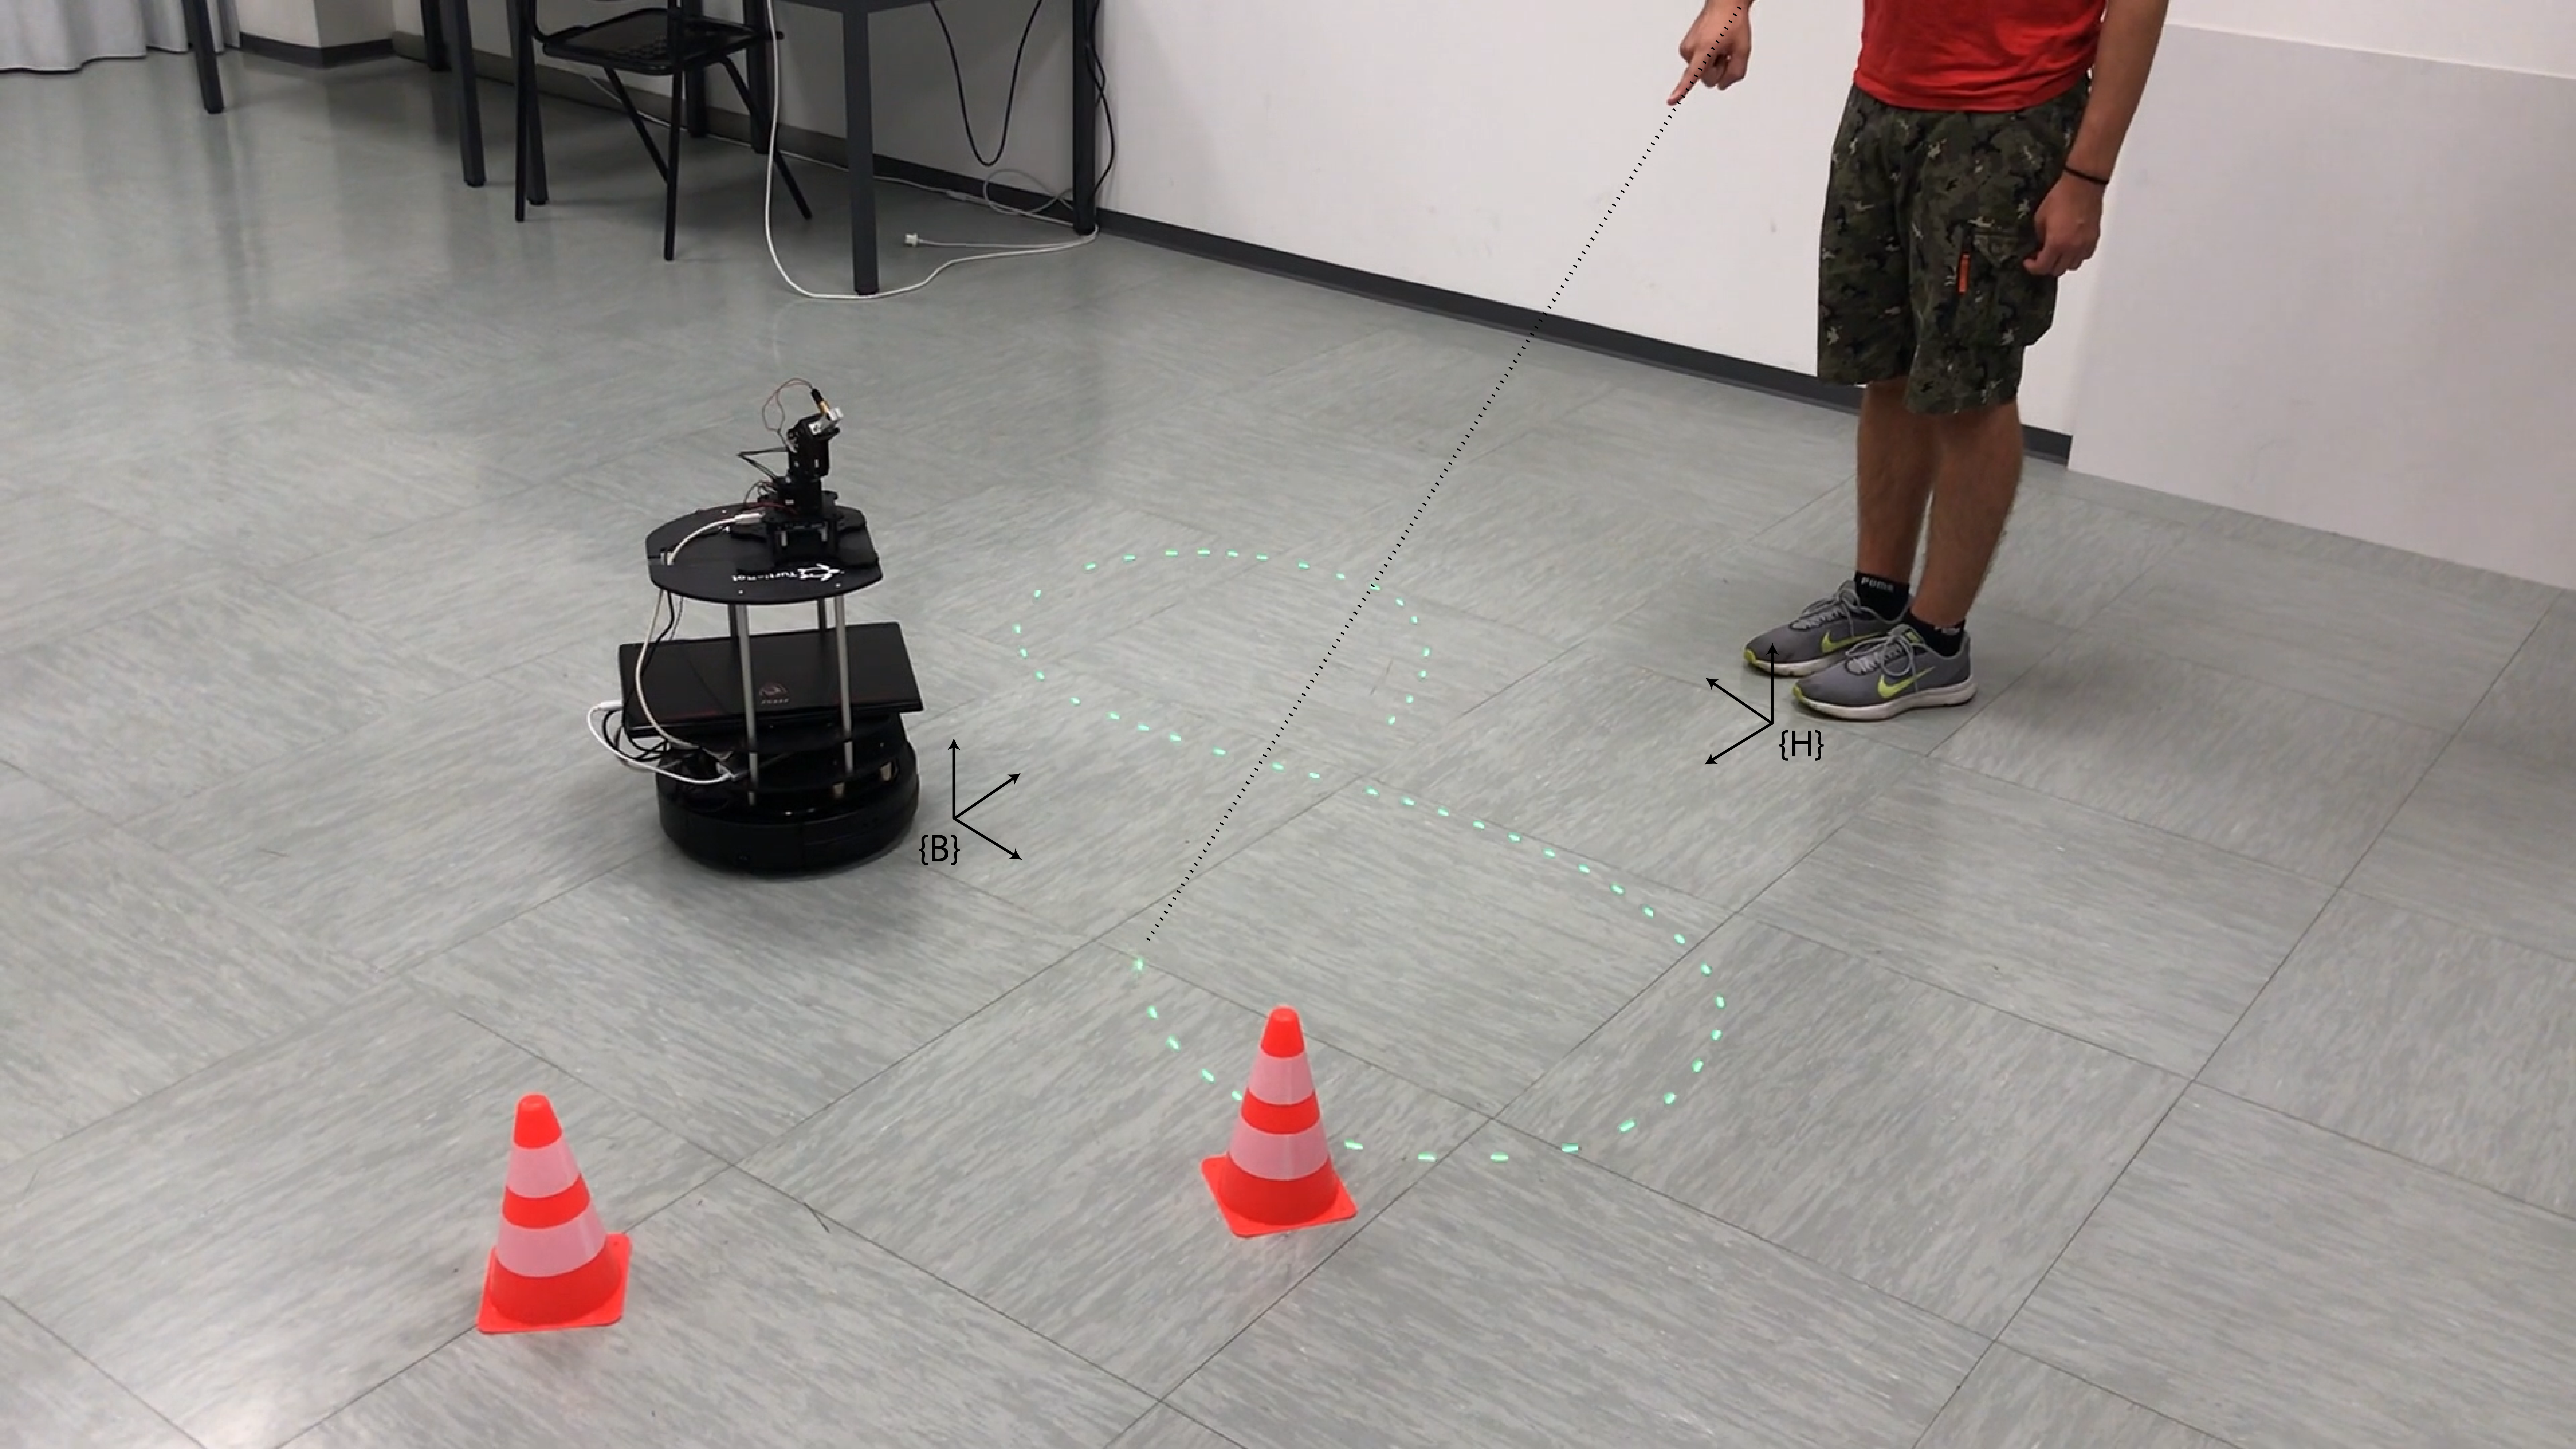
\includegraphics[width=\textwidth]{img/kgtgRelloc2.png}%
	\caption{Kobuki Go to Goal: User doing the Relloc. The laser shape trajectory is made visible.}
	\label{fig:kgtgRelloc}
\end{figure}
\begin{figure}
	\centering
	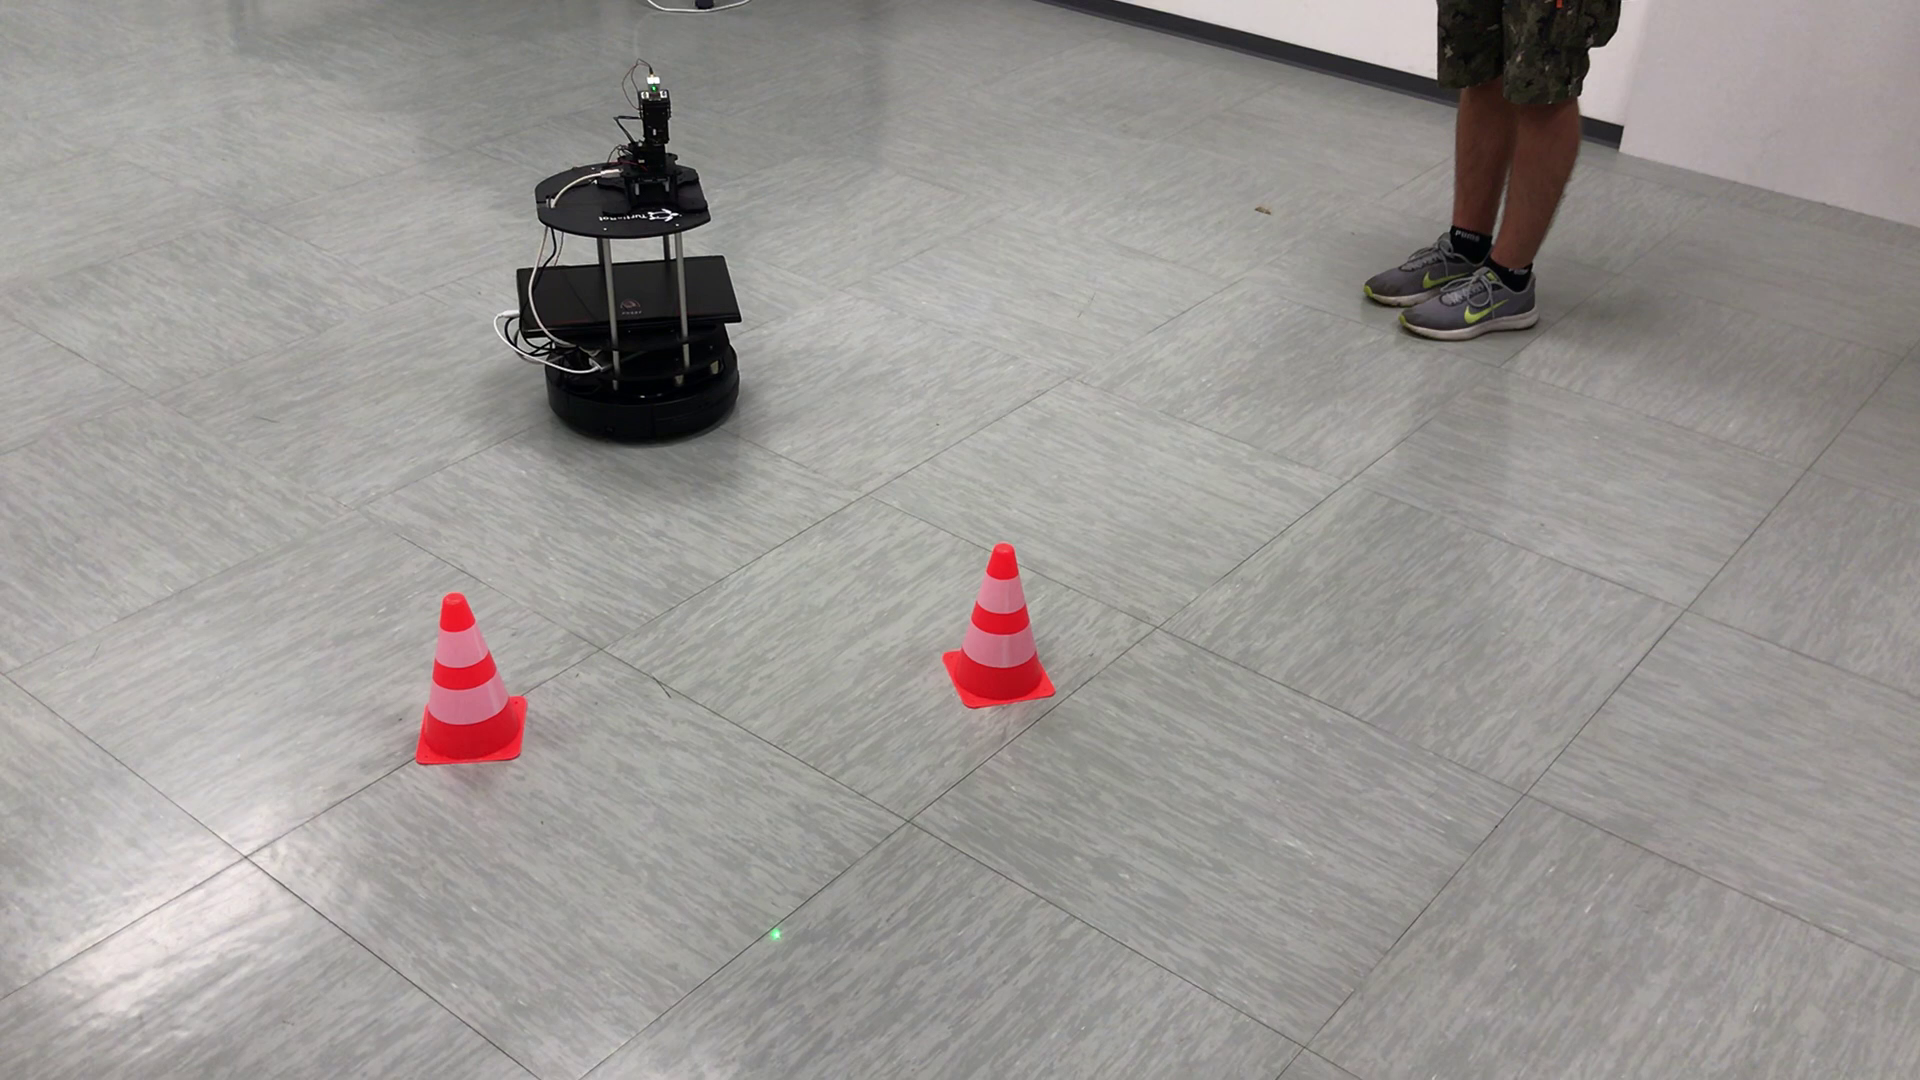
\includegraphics[width=\textwidth]{img/kgtgPointing.png}%
	\caption{Kobuki Go to Goal: Pointing Goal Point}
	\label{fig:kgtgPointing}
\end{figure}
\begin{figure}
	\centering
	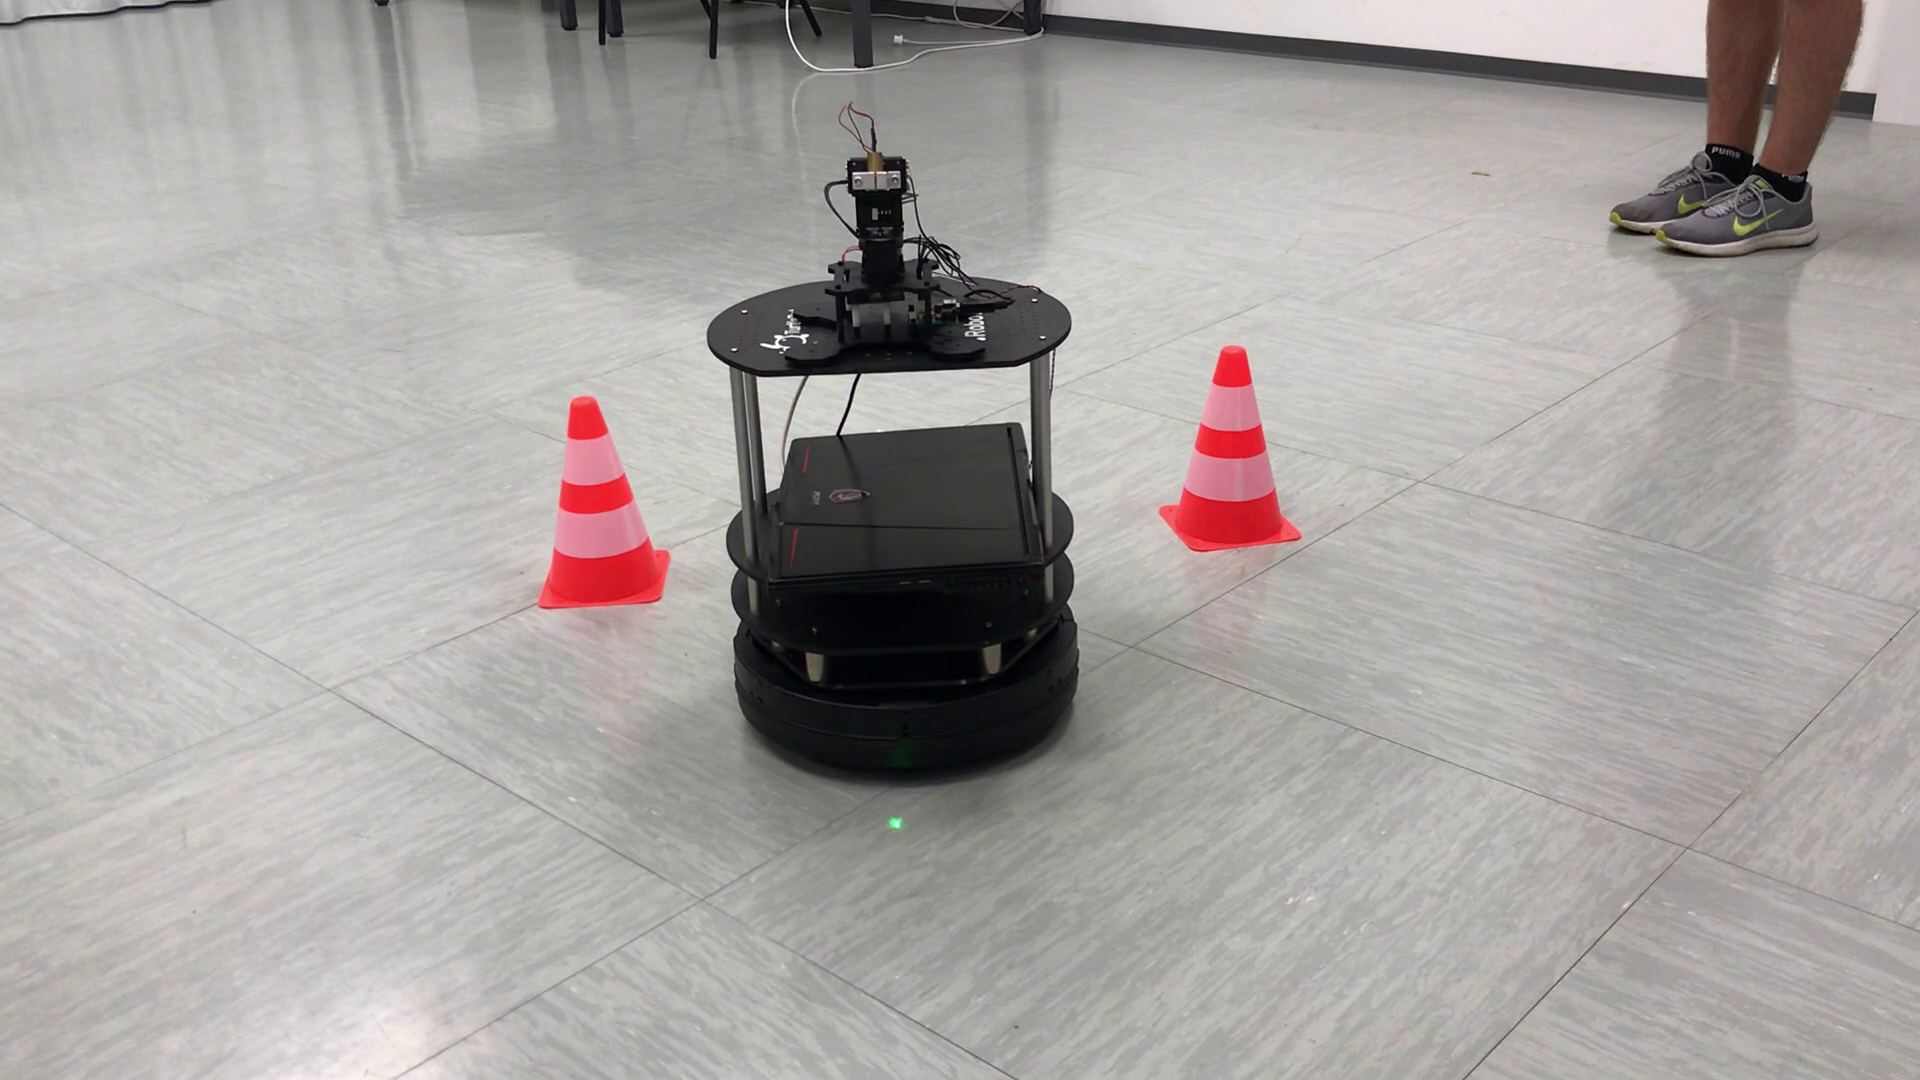
\includegraphics[width=.7\textwidth]{img/kgtgGoal.png}%
	\caption{Kobuki Go to Goal: Goal Point Reached}
	\label{fig:kgtgGoal}
\end{figure}
\begin{figure}
	\centering
	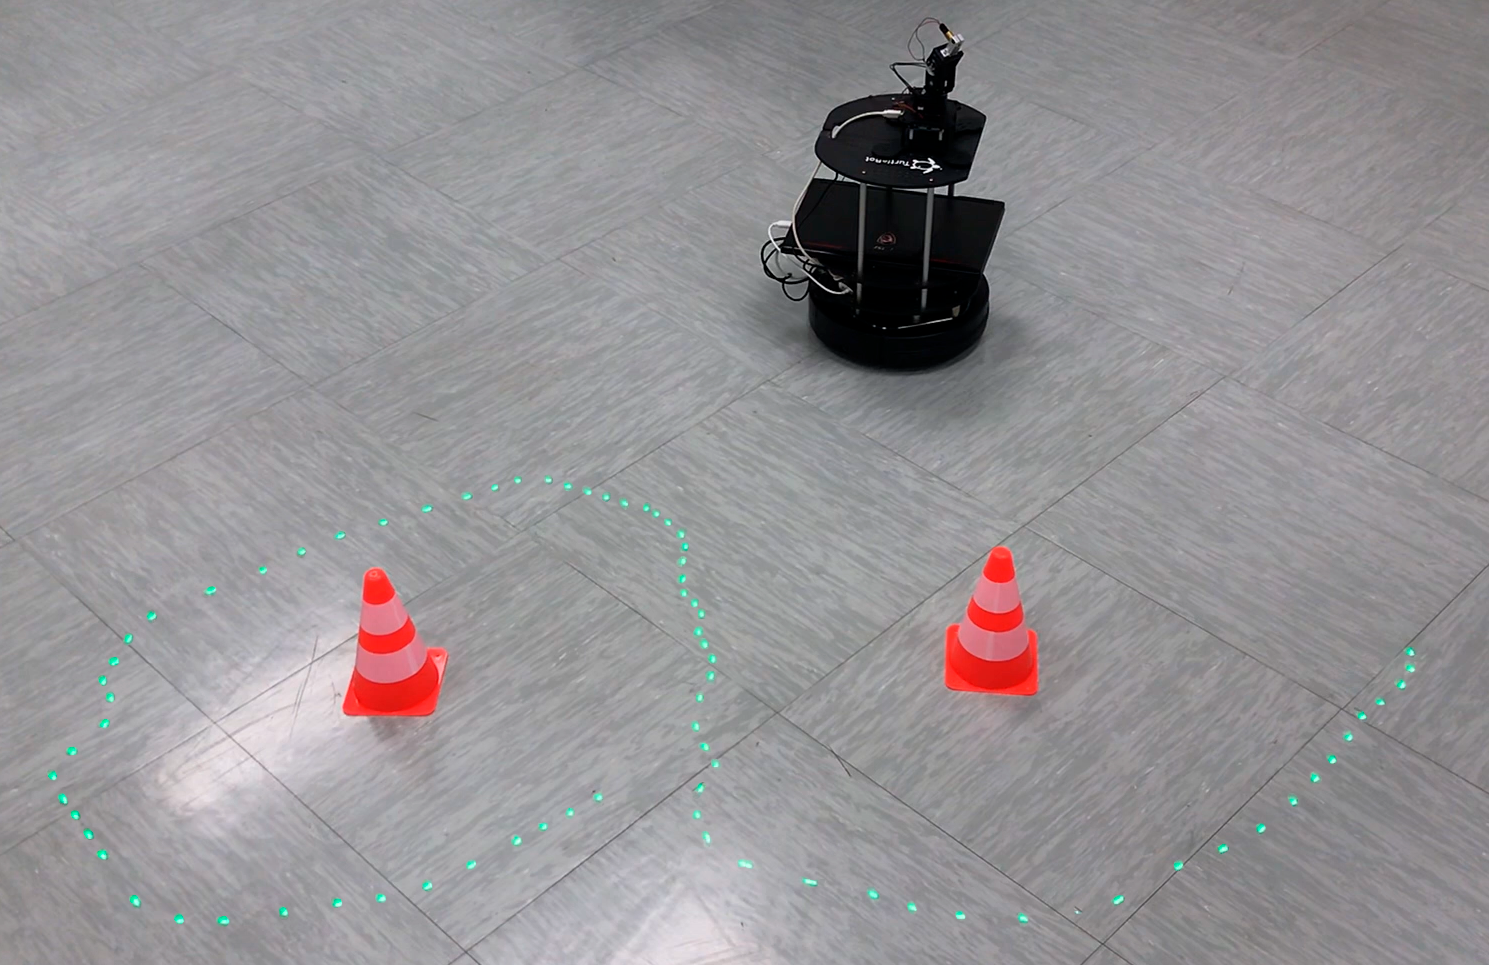
\includegraphics[width=.7\textwidth]{img/kftTrajectory.png}%
	\caption{Kobuki Follow Trajectory: User's Trajectory}
	\label{fig:kgtgGoal}
\end{figure}
%\chapter{Conclusions and Future Work} 
\label{chap:5} 
\section{Conclusions}
\subsection{The Turret}
The first step of this project is to develop a pan and tilt turret able to project a laser dot on a given surface and finely control its position by solving the inverse kinematics. That goal is achieved with two different models, that we have described in that thesis both in terms of geometrical model and hardware/software implementations. The result is that, with our first turret, we are able to fulfill all our goals in a proper way. However, the second model proves to be better in performances, since it allows us to control the laser with greater precision and smoothness, being built with more expensive and powerful servos.

\subsection{HRI Task}
With the functionality of the turret validated, we are able to deploy our system for a \ac{HRI} task. In fact, we integrate that work with an existing system in which an operator interacts with a drone using pointing gestures \cite{gromov2018robot}. That interaction approach is suitable for fast agile robot, able to follow indicated locations in real time, but does not fit for slower or larger ground robots. Our goal is to provide a usable interface for those latter cases with our turret. So, by mounting the turret on a kobuki, we are able to solve the robot navigation task efficiently, applying the relative localization approach to the aforementioned slow ground robot and driving it around exploiting the laser pointing. Applications developed show that our approach works well in practice, as users are able to drive the robot to a goal point or through a trajectory very precisely.

\subsection{Experiments}
Finally, the turret gives us the possibility to efficiently run experiments to validate our system components. In particular, we report two experiments: pointing experiment and \ac{relloc} experiment.

The first helps us to understand whether our over-simplified human pointing model is good enough to work well. The answer is yes, as results show. Moreover, it also points out the fact that users, with a feedback for their pointing, are able to compensate any intrinsic error or misalignment of the system, giving a strong confirmation to our work. This is not surprising, because is exactly one of the motivations that we highlights analyzing related works in \textit{\nameref{sec:related}} section.

The second is useful to asses the precision of the relative localization procedure. Moreover, that experiment was run with a group of unskilled people, so it is also an indicator of how easy the procedure is to be followed. Results are quite good, considering the fact that we had time to run the data collection campaign only with the first turret, which is less accurate. Demos we developed later, which deployed the \ac{relloc} with the new turret, give us qualitative evidences that this model is more precise and reliable. We even found out that performing the \ac{relloc} sometimes is more precise than manually setting the position of the user. This happens because measuring manually is of course prone to human error and, most important thing, does not take into account any inaccuracy of the system. The \ac{relloc} thing, on the contrary, takes place entirely within the system environment, so, when it is precise, is able to collocate the human within the system accurately.

\section{Future Work}
\subsection{Relloc and Pointing Experiments}
As already explained many times, the \ac{relloc} experiment was run only with the first turret model. We plan to conduct a data collection campaign with the second model. Being more precise, we expect to obtain better results and a more reliable indicator of the \ac{relloc} accuracy. If that intuition will prove to be true, we could also rethink the pointing experiment in such a way that we do not set the position of the human by hand, but we make him run the \ac{relloc} before starting with the data collection.
\subsection{Human Body Measures}
To allow users to use the system (e.g. to run experiments) we had to collect their physical data in order to build the human system properly. Since that procedure is time consuming and error prone, we would like to make it automatic. For example, we could determine approximate measures based on user's height and sex. Moreover, we could exploit the \ac{IMU} sensor to determine the height. That procedure would make interfacing with the system easier and faster for new users.

\subsection{Point to Wall (in Arbitrary Places)}
As already explained in section \ref{subs:floorwall}, we implemented the pipeline also to drive the laser on the wall, but there are some limitations. In fact, we have to explicitly set the distance of the turret from the wall and its relative orientation. A possible further development could help to remove that requirement. For example, we could equip the turret with a coaxial laser rangefinder with pointer. In that way, we could be able to determine those initial condition autonomously and thus the wall would not need to be \virgolette{calibrated} manually. That would allow the system to be deployed in arbitrary places.
%\input{./Chapters/Chapter6}

% ============================
%           APPENDICES
% ============================

\begin{appendices}
	\renewcommand*\appendixpagename{Appendices}
	\renewcommand*\appendixtocname{Appendices}
	\appendixpage
	\addappheadtotoc
	\chapter{}
\label{Appen:A}
In that appendix we discuss a couple of things that for different reasons are only mentioned in the main document, but can still be interesting.
\section{Motor Issues: Solution Attempts}
As we discussed in \ref{subs:firstModel:issues}, we had to face many issues with the Dynamixel AX-12+ servos. Many solutions were implemented before the right one, which is explained in the thesis. Here we give an overview of all those attempts as, even if none of them completely solved our issues, developing them and understand why they were not working was a huge part of that thesis work, so they are worth to be mentioned. Here comes a brief list:
\paragraph{ROS Library:} changing the library for ROS, using both official and unofficial. It did not help because as, how it turned out later, we had a driver problem;
\paragraph{Wheel Mode vs Joint Mode:} those servos have the possibility to directly control their velocity (wheel mode) and not their position (joint mode, default behaviour). Thus, we implemented an open loop controller in wheel mode: that means that we compute for how long the motor must move at a certain speed to reach a given position. That was possible thanks to an external library, but it turned out that Dynamixels AX-12+ does not have a true speed controller, but just a PWM controller. That makes even harder to control the motors, as one would have to be able to compute how much power is needed to move the motor at a certain speed under certain conditions (e.g. load);
\paragraph{PID Controller:} again using wheel mode, we tried to build a PID controller, but since the communication with the turret was very slow, that did not improve things;
\paragraph{PID, Joint Mode:} we even tried a PID controller in joint mode, though it did not make much sense;
\paragraph{Compliance Slope and Margin:} those servos have two internal parameters. \emph{Compliance} is to set the control flexibility of the motor.
Diagram in figure \ref{fig:compliance} shows the relationship between output torque and position of the motor. \emph{Compliance Margin} exists in each direction of \acs{CW}/\acs{CCW} and means the error between goal position and present position. The greater the value, the more difference occurs. \emph{Compliance Slope} sets the level of Torque near the goal position, the higher the value, the more flexibility is obtained.
\begin{figure}
	\centering
	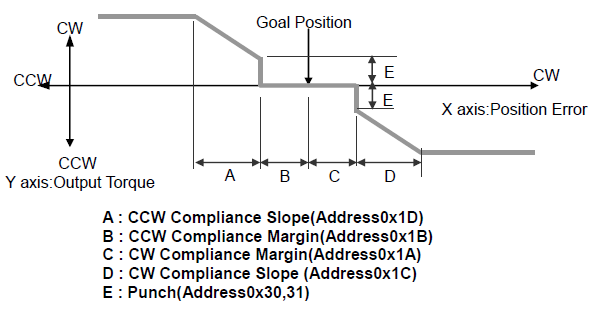
\includegraphics[width=\textwidth]{img/compliance.png}%
	\caption{Compliance Slope and Margin}
	\label{fig:compliance}
\end{figure}
Changing those values allowed us to obtain smoother trajectories, but sacrificing precision which, at the earlier stage was not important and not visible, but it could not be tolerate when implementing the relative localization system, as being imprecise with the laser pointer directly affects system performances.


\section{Motor Frames Mounting Instructions}
For sake of completeness, we include the instructions followed to mount the motors together.

Figure \ref{fig:axMounting2} shows how the \texttt{F3} is used to attach two dynamixels AX-12 together. In that way, we implement our pan component, since the bottom motor (the one on the left in the picture) can rotate the base of the upper one. Figure \ref{fig:s101Mounting} shows how the same thing can be obtained with two MX-64 servos and a \texttt{SR05-H101} frame.
\begin{figure}
	\centering
	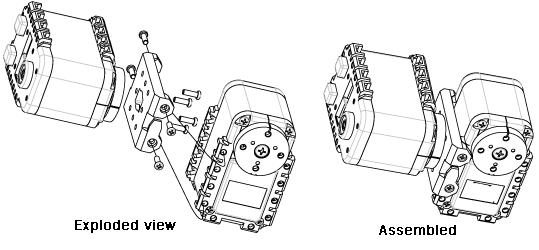
\includegraphics[width=.7\textwidth]{img/axMounting2.png}%
	\caption{Mounting F3 Frame}
	\label{fig:axMounting2}
\end{figure}
\begin{figure}
	\centering
	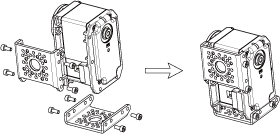
\includegraphics[width=.7\textwidth]{img/rx-64_fr05-s101.png}%
	\caption{Mounting FR05-S101 Side Frame}
	\label{fig:s101Mounting}
\end{figure}

Figure \ref{fig:axMounting1} shows how to mount the \texttt{F2} frame on top of a AX-12 servo. This is the physical representation of our tilt angle, as we mount the laser diode exactly in the middle of that frame. This is very convenient since, as already discussed, mounting the laser in that way simplifies the inverse kinematic very much. Figure \ref{fig:h101Mounting} shows the same with a \texttt{FR05-H101} hinge frame and a MX-64 motor. Note that since that frame is slightly shorter than the \texttt{F2} counterpart, we have to mount laser differently on that motor, obtaining a different and a bit more complex inverse kinematic
\begin{figure}
	\centering
	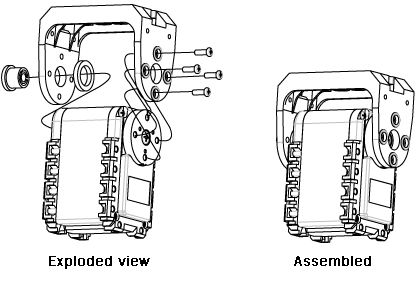
\includegraphics[width=.7\textwidth]{img/axMounting1.png}%
	\caption{Mounting F2 Frame}
	\label{fig:axMounting1}
\end{figure}


\begin{figure}
	\centering
	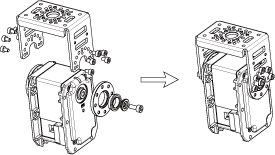
\includegraphics[width=.7\textwidth]{img/rx-64_fr05-h101.png}%
	\caption{Mounting FR05-H101 Hinge Frame}
	\label{fig:h101Mounting}
\end{figure}

\section{Data Analysis Pipeline}
In the experiment section in chapter \ref{chap:4} we analyze and report the result obtained with our experiments. Here we want to describe the pipeline built to collect those data, put them together and analyze them.

Of course, the main part regard data collection. Thank to ROS, we were able to recorder entire sessions from each user. \textit{Entire} means that we can store in bag files every single message sent through ROS and then analyze the data offline or even replay the entire experiment.

From the collected bag file, we extract all the messages relevant for the experiment and store them as \texttt{pandas} dataframes. For that, a library was provided.

Here are the main topics extracted for each experiment:

\textbf{pointing experiment}:
\begin{itemize}
    \item \texttt{arm\_pointer}, containing estimated 3D points on the ground pointed by the human (in human frame);
    \item \texttt{laser\_point}, containing 3D points of the laser dot;
    \item \texttt{target\_point}, containing 3D points of the targets on the ground (published just for convenience);
\end{itemize}
\textbf{relloc experiment}:
\begin{itemize}
    \item \texttt{relloc\_human\_pose}, containing estimated 3D points of the human in the turret frame, computed and published for application purposes;
    \item \texttt{gt\_point}, containing 3D ground truth points, i.e. the points where the user should stand when doing the relloc. We need to publish since they are randomly shuffled for each user, thus we cannot assume that we already know them.
\end{itemize}
Given that, is easy to understand how we obtain the results discussed in chapter \ref{chap:4}. For the pointing experiment, we confront \texttt{arm\_pointer} points with \texttt{laser\_point} ones, considering also their distances from the targets for each session. For the relloc one, for each session we compute the distance between the ground truth point and the estimated one.

It is also worth to say that the aforementioned concept of \textit{session} needed a bit of work to be implemented, as each dataframe needed to be parsed and each session distinguished from the others. To do that easily, we implemented a machine state mechanism which publishes a string message over a ROS topic containing the current state of the system. With a clever use of that concept, we are able to mark the begin and the end of each session and then recover it when parsing the data.

To conclude, we can add that the code to parse the data, analyze and print/plot results is available as convenient \texttt{ipython} notebooks. In that way, we can easily run and analyze new data eventually collected.	
	\chapter{Other Listings}
\label{Appen:B}
Other listings excluded from the text for better readability.
\subsection*{\texttt{find\_nearest} method}
\begin{lstlisting}[caption={Find Nearest function},label={lst:nearest},language=Python]
def find_nearest(array, value):
	"""
		find nearest value in array
	Args:
		array: array of values
	value: reference value
	
	Returns:
		min index of nearest array's element to value
	"""
	return (np.abs(array - value)).argmin()
\end{lstlisting}
\subsection*{\texttt{change\_frame\_reference} method}
\begin{lstlisting}[caption={Change frame of reference},label={lst:changeframe},language=Python]
def change_frame_reference(pose_bebop, pose_head):
	"""
		Change frame of reference of pose head from World to bebop.
	
	Args:
		pose_bebop: pose of the bebop
		pose_head: pose of the head
	
	Returns:
		the new pose for head:
			bebop
				T
				head
	"""
	position_bebop = pose_bebop[['b_pos_x', 'b_pos_y', 'b_pos_z']].values
	quaternion_bebop = pose_bebop[['b_rot_w', 'b_rot_x', 'b_rot_y', 'b_rot_z']].values
	position_head = pose_head[['h_pos_x', 'h_pos_y', 'h_pos_z']].values
	quaternion_head = pose_head[['h_rot_w', 'h_rot_x', 'h_rot_y', 'h_rot_z']].values
	w_t_b = rospose2homogmat(position_bebop, quaternion_bebop)
	w_t_h = rospose2homogmat(position_head, quaternion_head)
	b_t_w = np.linalg.inv(w_t_b)
	b_t_h = np.matmul(b_t_w, w_t_h)
	
	return b_t_h
\end{lstlisting}
\subsection*{\texttt{VideoCreator} Class}
\begin{lstlisting}[caption={Video creator class},label={lst:videocreator},language=Python]
class VideoCreator:
	def __init__(self, b_orientation, distances, b_position, frame_list, h_orientation, h_position, delta_z, f, title="test.avi"):
		"""
			Initializer for the class
		Args:
			distances: list of distance user-drone
			b_orientation: bebop orientation array
			b_position: bebop position array
			frame_list: camera frame list
			h_orientation: head orientation array
			h_position: head orientation array
			delta_z: height difference list
			f: bag file name
			title: video file name
		"""
		self.fps = 30
		self.f = f
		self.video_writer = cv2.VideoWriter(title, cv2.VideoWriter_fourcc(*'XVID'), self.fps, (640, 480))
		self.b_orientation = b_orientation
		self.b_position = b_position
		self.frame_list = frame_list
		self.h_orientation = h_orientation
		self.h_position = h_position
		self.distances = distances
		self.delta_z = delta_z
	
	def plotting_function(self, i):
		"""
			Given an index compose the frame for the video.
		Args:
			i: frame number
		"""
		fig = plt.figure()
		fig.suptitle("Frame: " + str(i), fontsize=12)
		axll = fig.add_subplot(2, 2, 1)
		axl = fig.add_subplot(2, 2, 2)
		axc = fig.add_subplot(2, 2, 3)
		axr = fig.add_subplot(2, 2, 4)
		canvas = FigureCanvas(fig)
		
		# Central image: here we add the camera feed to the video
		img = Image.open(io.BytesIO(self.frame_list[i]))
		raw_frame = list(img.getdata())
		frame = []
		for b in raw_frame:
		frame.append(b)
		reshaped_fr = np.reshape(np.array(frame, dtype=np.int64), (480, 856, 3))
		reshaped_fr = reshaped_fr.astype(np.uint8)
		axc.imshow(reshaped_fr)
		axc.set_axis_off()
		
		# RIGHT PLOT: here we create the right plot that represent the position and heading of the bebop and head
		axr.axis([-2.4, 2.4, -2.4, 2.4], 'equals')
		h_theta = quat_to_eul(self.h_orientation[i])[2]
		b_theta = quat_to_eul(self.b_orientation[i])[2]
		arrow_length = 0.3
		spacing = 1.2
		minor_locator = MultipleLocator(spacing)
		# Set minor tick locations.
		axr.yaxis.set_minor_locator(minor_locator)
		axr.xaxis.set_minor_locator(minor_locator)
		# Set grid to use minor tick locations.
		axr.grid(which='minor')
		axr.plot(self.b_position[i].x, self.b_position[i].y, "ro", self.h_position[i].x, self.h_position[i].y, "go")
		axr.arrow(self.h_position[i].x, self.h_position[i].y, arrow_length * np.cos(h_theta), arrow_length * np.sin(h_theta), head_width=0.05, head_length=0.1, fc='g', ec='g')
		axr.arrow(self.b_position[i].x, self.b_position[i].y, arrow_length * np.cos(b_theta), arrow_length * np.sin(b_theta), head_width=0.05, head_length=0.1, fc='r', ec='r')
		
		# LEFT PLOT: here we represent the distance on the y axis and the heading correction for the drone in degrees on the x-axis
		r_t_h = matrix_method(self.b_position[i], self.b_orientation[i], self.h_position[i], self.h_orientation[i])
		horizontal_angle = -math.degrees(math.atan2(r_t_h[1, 3], r_t_h[0, 3]))
		
		value_angle_axis = 45
		axl.set_xlim(-value_angle_axis, value_angle_axis)
		axl.set_ylim(0.1, 3)
		axl.set_xlabel('Angle y')
		axl.set_ylabel('Distance')
		axl.plot(horizontal_angle, self.distances[i], 'go')
		
		axll.set_xlim(-value_angle_axis, value_angle_axis)
		axll.set_ylim(-1, 1)
		axll.set_xlabel('Angle y')
		axll.set_ylabel('Delta z')
		axll.plot(horizontal_angle, self.delta_z[i], 'go')
		# Drawing the plot
		canvas.draw()
		
		# some additional informations as arrows
		width, height = (fig.get_size_inches() * fig.get_dpi()).astype(dtype='int32')
		img = np.fromstring(canvas.tostring_rgb(), dtype='uint8').reshape(height, width, 3)
		img = cv2.cvtColor(img, cv2.COLOR_RGB2BGR)
		pt1 = (275, 40)
		pt2 = (375, 40)
		if horizontal_angle >= 0:
			cv2.arrowedLine(img, pt1, pt2, (0, 0, 255), 3)
		else:
			cv2.arrowedLine(img, pt2, pt1, (0, 0, 255), 3)
		
		pt3 = (25, 175)
		pt4 = (25, 225)
		if self.distances[i] < 1.5:
			cv2.arrowedLine(img, pt3, pt4, (0, 255, 0), 3)
		else:
			cv2.arrowedLine(img, pt4, pt3, (0, 255, 0), 3)
		
		self.video_writer.write(img)
		plt.close(fig)
	
	def video_plot_creator(self):
		"""
			calls frame composers for every frame
			complete video creation
		"""
		max_ = len(self.frame_list)
		for i in tqdm.tqdm(range(0, max_)):
			self.plotting_function(i)
		self.video_writer.release()
		cv2.destroyAllWindows()
\end{lstlisting}
\subsection*{\texttt{keras\_train} Script}
%\lstinputlisting[caption={\texttt{keras\_train} Script},label={lst:kerastrain},language=Python]{code/kerastrain.py}
\subsection*{\texttt{keras\_crossvalidation} Script}
%\lstinputlisting[caption={\texttt{keras\_crossvalidation} Script},label={lst:kerascross},language=Python]{code/kerascrossvalidation.py}
\subsection*{\texttt{model\_creator} Script}
%\lstinputlisting[caption={\texttt{model\_creator} Script},label={lst:modelcreator},language=Python]{code/modelcreator.py}
\subsection*{\texttt{bag\_to\_pickle} Method}
\begin{lstlisting}[caption={Extract that shows the method \text{bag\_to\_pickle}},label={lst:bagtopickle},language=Python]
def bag_to_pickle(f):
"""
Core method used to transforms and saves a bag file into a .pickle dataset file
Args:
f: file name e.g. "7.bag"
"""
path = bag_file_path[f[:-4]]
print("\nreading bag: " + str(f))
datacr = DatasetCreator()
with rosbag.Bag(path + f) as bag:
bag_df_dict = get_bag_data_pandas(bag)
data_vec = processing(bag_df_dict=bag_df_dict, data_id=f[:-4], f=f)
datacr.generate_data(data_vec=data_vec)
datacr.save_dataset(flag_train="cross", title=f[:-4] + ".pickle")

print("\nCompleted pickle " + str(f[:-4]))
\end{lstlisting}
\subsection*{\texttt{processing} Method}
\begin{lstlisting}[caption={\texttt{processing}} method,label={lst:processing},language=Python]
def processing(bag_df_dict, data_id, f):
"""
Process data from dictionary bag_df_dict into a data vector
Args:
bag_df_dict: dictionary of Pandas dataframes
data_id: id of the bag file processed
f: bag file name, used as key for dictionary
Returns:
data vector: vector of tutples (image, (targe_x, target_y, target_z, target_relative_yaw)
"""
camera_t = bag_df_dict["camera_df"].index.values
bebop_t = bag_df_dict["bebop_df"].index.values
head_t = bag_df_dict["head_df"].index.values
data_vec = []
max_ = bag_end_cut[f[:-4]]
min_ = bag_start_cut[f[:-4]]
for i in tqdm.tqdm(range(min_, max_), desc="processing data " + str(data_id)):
b_id = find_nearest(bebop_t, camera_t[i])
h_id = find_nearest(head_t, camera_t[i])
head_pose = bag_df_dict["head_df"].iloc[h_id]
bebop_pose = bag_df_dict["bebop_df"].iloc[b_id]
img = bag_df_dict["camera_df"].iloc[i].values[0]
b_t_h = change_frame_reference(bebop_pose, head_pose)
quaternion_bebop = bebop_pose[['b_rot_x', 'b_rot_y', 'b_rot_z', 'b_rot_w']].values
quaternion_head = head_pose[['h_rot_x', 'h_rot_y', 'h_rot_z', 'h_rot_w']].values
_, _, head_yaw = quat_to_eul(quaternion_head)
_, _, bebop_yaw = quat_to_eul(quaternion_bebop)
relative_yaw = (head_yaw - bebop_yaw - np.pi)
if relative_yaw < -np.pi:
relative_yaw += 2 * np.pi
target_position = b_t_h[:-1, -1:].T[0]
target = (target_position[0], target_position[1], target_position[2], relative_yaw)
data_vec.append((img, target))
return data_vec
\end{lstlisting}
\subsection*{\texttt{dumb\_regressor} Script}
%\lstinputlisting[caption={\texttt{dumb\_regressor} Script},label={lst:dumbreg},language=Python]{code/dumbregressor.py}	
\end{appendices}

% ============================
%          REFERENCES
% ============================

\clearpage
\addcontentsline{toc}{chapter}{References}
\renewcommand\bibname{References}
\bibliography{references}
\bibliographystyle{ieeetr}
\fancyhead[L]{}
\fancyhead[R]{\slshape References}

% ============================
%           ACRONYMS
% ============================

\phantomsection
\chapter*{Acronyms\markboth{Acronyms}{}} 
\addcontentsline{toc}{chapter}{Acronyms}
\small
\begin{acronym}[OpenCV] % insert in the square brackets the longest acronym word
    \acro{CNN}[CNN]{Convolutional Neural Network}
    \acro{ROS}[ROS]{Robot Operating System}
    \acro{HRI}[HRI]{Human-Robot Interaction}
    \acro{NN}[NN]{Neural Network}
    \acro{FOV}[FOV]{Field of View}
    \acro{MoCap}[MoCap]{Motion Capture}
    \acro{IDSIA}[IDSIA]{Istituto Dalle Molle di Studi sull'Intelligenza Artificiale}
    \acro{RNN}[RNN]{Recurrent Neural Network}
    \acro{OS}[OS]{Operating System}
    \acro{WLAN}[WLAN]{Wireless Local Area Network}
    \acro{MIMO}[MIMO]{Multiple-Input and Multiple-Output}
    \acro{GNSS}[GNSS]{Global Navigation Satellite System}
    \acro{GPS}[GPS]{Global Positioning system}
    \acro{AIDA}[AIDA]{Artificial Intelligence for Drone Auto-follow}
    \acro{wrt.}[wrt.]{with respect to}
    \acro{IR}[IR]{Infrared}
    \acro{ReLU}[ReLU]{Rectified Linear Unit}
    \acro{MSE}[MSE]{Mean Squared Error}
    \acro{MAE}[MAE]{Mean Absolute Error}
    \acro{OpenCV}[OpenCV]{Open Source Computer Vision Library}
    \acro{ASIC}[ASIC]{Application Specific Integrated Circuit}
    \acro{DoF}[DoF]{Degree of Freedom}
    \acro{Adam}[Adam]{Adaptive Moment Estimation}
    \acro{SVM}[SVM]{Support Vector Machines}
\end{acronym}
\normalsize

\fancyhead[L]{}
\fancyhead[R]{\slshape Acronyms}	

%%=============================
%%		    THANKS	
%%=============================

\phantomsection
\chapter*{Thanks to\markboth{Thanks to}{}} 
\addcontentsline{toc}{chapter}{Thanks to}
I am finally writing the last page of this thesis and I would like to spend a few words to say thanks to all the people that were with me through this journey.\\

Thanks to my family. In particular my mother, my father and my brother. You are always there for me, even when, under pressure, I tend to make myself unbearable. Your support is truly important, I would not go far without it.\\

Thanks to my love, Valentina. Well, \virgolette{I don't even need to sugarcoat it}, right? You are part of my family by now, so... read above!\\

Thanks to Andrea, maybe my supporter number one (after my mother, of course). It was a while ago, but you convinced me that I am worthy of something.\\

Thanks to all my friends. I am lucky (or lazy?) enough to say that you are too many, so I cannot write all your names. However, if even only one time, you were patient enough to listen to me talking about that line of code I had written, then... thank you, that meant a lot!\\

Thanks to Boris, my thesis co-supervisor, my teaching assistant and my classmate. You were always kind and willing to help me. I learned a lot from you.\\

Thanks to Alessandro, for the opportunity of doing this thesis and the help you always kindly provided me.\\

Thanks to Professor Pezz\`e, Professor Denaro and double degree coordinators for the opportunity of this double degree.\\

And if you, who are reading now, if you think that I forgot to thank you, then... thank you! We good, right?
\fancyhead[L]{}
\fancyhead[R]{\slshape Thanks to}
	

\end{document}
